\documentclass[11pt,twoside,a4paper,openany]{report}
\usepackage[solcolor]{ex_test} % dethi, color, loigiai, solcolor, book
%\usepackage{ex_test}
\renewtheorem{ex}{\color{blue!60!black} Câu}
	\input{../extra/pkgs}
	\input{../extra/defs2}
%	\input{../extra/blank-text2}

\begin{document}
	
%	\tableofcontents
%	\cleardoublepage
%	\AnswersOn
	\AnswersOff
% ==================================LỚP 12 =================================================
%\setcounter{part}{0}
%\part{TỔNG HỢP KIẾN THỨC}
%\startcontents[parts]
%\printcontents[parts]{}{0}{\setcounter{tocdepth}{0}}
%\setcounter{mychapter}{0}
%\mychapter{VẬT LÍ NHIỆT}
%\startcontents[mychapters]
%\printcontents[mychapters]{}{0}{\setcounter{tocdepth}{1}}
%\begin{center}
%	\includegraphics[width=0.8\linewidth]{../figs/G12C1}
%\end{center}
%\chapter{Tóm tắt lý thuyết}
\section{Mô hình động học phân tử và sự chuyển thể}
\subsection{Mô hình động học phân tử}
\begin{itemize}
	\item Vật chất được cấu tạo từ các hạt riêng biệt gọi là phân tử.
	\item Các phân tử chuyển động hỗn loạn không ngừng, gọi là chuyển động nhiệt. Nhiệt độ càng cao thì tốc độ trung bình của các phân tử càng lớn.
	\item Giữa các phân tử có lực liên kết phân tử (hút và đẩy).
\end{itemize}
\subsection{Cấu trúc của vật chất}
\begin{center}
	\begin{tabular}{|L{4cm}|L{4cm}|L{4cm}|L{4cm}|}
		\hline
		\thead{Cấu trúc}&\thead{Thể khí}& \thead{Thể rắn}&\thead{Thể lỏng}\\
		\hline
		Khoảng cách giữa các phân tử & Rất xa nhau (gấp hàng chục lần kích thước phân tử) & Rất gần nhau (cỡ kích thước phân tử) & Xa nhau\\
		\hline
		Sự sắp xếp của các phân tử & 	Không có trật tự & Trật tự & Kém trật tự hơn thể rắn\\
		\hline
		Chuyển động của các phân tử & Chuyển động hỗn loạn & Chỉ dao động quanh vị trí cân bằng cố định & Dao động quanh vị trí cân bằng luôn thay đổi\\
		\hline
		Minh họa chuyển động của các phân tử & \begin{center}
			\includegraphics[width=0.8\linewidth]{../figs/G12C1-1}
		\end{center}&\begin{center}
		\includegraphics[width=0.8\linewidth]{../figs/G12C1-2}
		\end{center}(Chất rắn kết tinh) &\begin{center}
		\includegraphics[width=0.8\linewidth]{../figs/G12C1-3}
		\end{center}\\
		\hline
	\end{tabular}
\end{center}
\subsection{Các quá trình chuyển thể}
\begin{itemize}
	\item Các chất có thể chuyển từ thể này sang thể khác.
	\item Cấu trúc của chất thay đổi khi chuyển thể.
\end{itemize}
\begin{center}
	\includegraphics[width=0.35\linewidth]{../figs/G12C1-4}
\end{center}
\luuy{Sự hóa hơi thể hiện qua hai hình thức: sự bay hơi và sự sôi
\begin{itemize}
	\item Sự bay hơi là sự hóa hơi xảy ra trên bề mặt chất lỏng. Sự bay hơi xảy ra ở bất kì nhiệt độ nào.
	\item Sự sôi là sự hóa hơi xảy ra ở bên trong và trên bề mặt chất lỏng. Sự sôi xảy ra ở nhiệt độ sôi.
	\end{itemize}}
\section{Nội năng - Định luật I nhiệt động lực học}
\subsection{Nội năng}
\begin{itemize}
	\item Nội năng của một vật là tổng động năng và thế năng tương tác của các phân tử cấu tạo nên vật.
	\item Nội năng được kí hiệu là $U$ và có đơn vị là $\si{\joule}$.
	\item Nội năng của vật phụ thuộc vào nhiệt độ $T$ và thể tích $V$ của vật.
	\item Có thể làm thay đổi nội năng của vật bằng cách: thực hiện công, truyền nhiệt.
\end{itemize}
\subsection{Định luật I nhiệt động lực học}
Độ biến thiên nội năng của vật bằng tổng công và nhiệt lượng mà vật nhận được.
\begin{equation}
	\Delta U=Q+A
\end{equation}
\begin{center}
	\includegraphics[width=0.3\linewidth]{../figs/G12C1-5}
\end{center}
\section{Thang nhiệt độ}
\subsection{Chiều truyền năng lượng nhiệt giữa hai vật chênh lệch nhiệt độ tiếp xúc nhau}
\begin{itemize}
	\item Khi hai vật chênh lệch nhiệt độ tiếp xúc nhau, năng lượng nhiệt luôn truyền từ vật có nhiệt độ cao hơn sang vật có nhiệt độ thấp hơn.
	\item Quá trình truyền nhiệt kết thúc khi hai vật ở cùng một nhiệt độ (cân bằng nhiệt với nhau).
\end{itemize}
\subsection{Các thang nhiệt độ}
\begin{itemize}
	\item \textit{Thang nhiệt độ Celsius}: Nhiệt độ đóng băng của nước tinh khiết là $\SI{0}{\celsius}$ và nhiệt độ sôi của nước tinh khiết là $\SI{100}{\celsius}$ ở áp suất tiêu chuẩn. Nhiệt độ trong thang Celsius thường được kí hiệu là $t$.
	\item \textit{Thang nhiệt độ Kelvin}: Nhiệt độ thấp nhất mà các vật có thể có được là $\SI{0}{\kelvin}$ (độ không tuyệt đối) và nhiệt độ mà nước tinh khiết có thể tồn tại đồng thời ở cả ba thể rắn, lỏng và hơi là $\SI{273.16}{\kelvin}$. Nhiệt độ trong thang Kelvin thường được kí hiệu là $T$.
	\begin{equation}
		\xsi{T}{\left(\si{\kelvin}\right)}=\xsi{t}{\left(\si{\celsius}\right)}+273
	\end{equation}
	
\end{itemize}
\manatip{Công thức chuyển đổi thang nhiệt độ $X$ sang thang nhiệt độ $Z$ có nhiệt độ đóng băng và nhiệt độ sôi  của nước tinh khiết lần lượt là $\left(X_b,X_s\right)$, $\left(Z_b, Z_s\right)$ trong trường hợp 2 thang nhiệt độ quan hệ tuyến tính với nhau:
	\begin{equation}
		\dfrac{X-X_b}{X_s-X_b}=\dfrac{Y-Y_b}{Y_s-Y_b}
	\end{equation}
	
}
\subsection{Nhiệt độ không tuyệt đối}
Nhiệt độ không tuyệt đối $\left(\SI{0}{\kelvin}\right)$ là nhiệt độ mà tại đó tất cả các chất có động năng chuyển động nhiệt của các phân tử hoặc nguyên tử bằng không và thế năng của chúng là tối thiểu.
\section{Nhiệt dung riêng, nhiệt nóng chảy riêng, nhiệt hóa hơi riêng}
\subsection{Nhiệt dung riêng}
\begin{itemize}
	\item Nhiệt dung riêng của một chất có giá trị bằng nhiệt lượng cần cung cấp để làm tăng nhiệt độ của $\SI{1}{\kilogram}$ chất đó lên $\SI{1}{\kelvin}$.
	\begin{equation}
		c=\dfrac{Q}{m\left(T_2-T_1\right)}
	\end{equation}
	\item Trong hệ SI, đơn vị đo nhiệt dung riêng là $\si{\joule/\left(\kilogram\cdot\kelvin\right)}$.
\end{itemize}
Nhiệt lượng mà một vật có khối lượng $m$ trao đổi khi thay đổi nhiệt độ từ $T_1$ đến $T_2$ được xác định bởi biểu thức: $Q = mc\left(T_2 – T_1\right)$\\
Trong hệ SI, đơn vị đo nhiệt lượng là $\si{\joule}$. Ngoài ra, nhiệt lượng còn được đo bằng đơn vị $\si{cal}$
$$\SI{1}{cal}=\SI{4,186}{\joule}.$$
\subsection{Nhiệt nóng chảy riêng}
\begin{itemize}
	\item Nhiệt nóng chảy riêng của một chất có giá trị bằng nhiệt lượng cần cung cấp cho $\SI{1}{\kilogram}$ chất đó chuyển hoàn toàn từ thể rắn sang thể lỏng tại nhiệt độ nóng chảy.\\
	\begin{equation}
		\lambda=\dfrac{Q}{m}
	\end{equation}
	\item Trong hệ SI, đơn vị đo nhiệt nóng chảy riêng là $\si{\joule/\kilo}$.
\end{itemize}
\subsection{Nhiệt hóa hơi riêng}
\begin{itemize}
	\item Nhiệt hoá hơi riêng của một chất lỏng có giá trị bằng nhiệt lượng cần cung cấp cho $\SI{1}{\kilogram}$ chất lỏng đó hoá hơi hoàn toàn ở nhiệt độ sôi.
	\begin{equation}
		L=\dfrac{Q}{m}
	\end{equation}
	\item Trong hệ SI, đơn vị đo nhiệt hoá hơi riêng là $\si{\joule/\kilogram}$.
\end{itemize}

%\chapter{Câu hỏi ôn tập}
\hideall{
	\setcounter{section}{0}
	\begin{center}
		\textbf{\large BẢNG ĐÁP ÁN}
	\end{center}
	\section{Câu trắc nghiệm nhiều phương án lựa chọn}
	\inputansbox{10}{ans/Y24-VN12-PH-C1-TN}
	\section{Câu trắc nghiệm đúng sai}
	\inputansbox[2]{2}{ans/Y24-VN12-PH-C1-TF}
	\section{Câu trắc nghiệm trả lời ngắn}
	\inputansbox[3]{6}{ans/Y24-VN12-PH-C1-TL}
}
\setcounter{section}{0}
\section{Câu trắc nghiệm nhiều phương án lựa chọn}
\textit{Thí sinh trả lời từ câu 1 đến câu 18. Mỗi câu thí sinh chọn một phương án}
\setcounter{ex}{0}
\Opensolutionfile{ans}[ans/Y24-VN12-PH-C1-TN]
% ===================================================================
\begin{ex}
	Chất rắn vô định hình là chất rắn
	\choice
	{có cấu trúc tinh thể}
	{\True không có cấu trúc tinh thể}
	{có nhiệt độ nóng chảy xác định}
	{có thể tích thay đổi}
	\loigiai{}
\end{ex}
% ===================================================================
\begin{ex}
	Tính chất nào sau đây \textbf{không phải} là tính chất của các phân tử khí?
	\choice
	{Có vận tốc trung bình phụ thuộc vào nhiệt độ}
	{Gây áp suất lên thành bình}
	{\True Chuyển động xung quanh vị trí cân bằng}
	{Chuyển động nhiệt hỗn loạn}
	\loigiai{}
\end{ex}
% ===================================================================
\begin{ex}
	Sự bay hơi
	\choice
	{\True xảy ra ở bất kì nhiệt độ nào của chất lỏng}
	{chỉ xảy ra ở trong lòng chất lỏng}
	{xảy ra với tốc độ như nhau ở mọi nhiệt độ}
	{chỉ xảy ra đối với một số ít chất lỏng}
	\loigiai{}
\end{ex}
% ===================================================================
\begin{ex}
	Đơn vị của nhiệt dung riêng là
		\choice
	{$\si{\joule/\kilogram}$}
	{$\si{\kilogram/\joule}$}
	{\True $\si{\joule/\kilogram\cdot\kelvin}$}
	{$\si{\kilogram/\joule\cdot\kelvin}$}
	\loigiai{}
\end{ex}
% ===================================================================
\begin{ex}
	Phát biểu nào sau đây là \textbf{sai}?
	\choice
	{Nhiệt độ sôi của chất lỏng phụ thuộc vào áp suất khí phía trên bề mặt chất lỏng}
	{Áp suất khí càng cao thì nhiệt độ sôi của chất lỏng càng cao}
	{\True Áp suất khí càng nhỏ thì nhiệt độ sôi của chất lỏng càng cao.}
	{Ở một áp suất nhất định, mỗi chất lỏng sôi ở nhiệt độ xác định và không đổi}
	\loigiai{}
\end{ex}
% ===================================================================
\begin{ex}
Nội năng của một vật là	
	\choice
	{tổng động năng chuyển động nhiệt của các phân tử cấu tạo nên vật}
	{\True tổng động năng và thế năng của các phân tử cấu tạo nên vật}
	{tổng nhiệt năng và cơ năng mà vật nhận được trong quá trình truyền nhiệt và thực hiện công}
	{nhiệt lượng vật nhận được trong quá trình truyền nhiệt}
	\loigiai{}
\end{ex}
% ===================================================================
\begin{ex}
	Nhiệt hóa hơi riêng của một chất lỏng là nhiệt lượng cần thiết để
	\choice
	{\True làm cho một kilogram chất lỏng đó hóa hơi hoàn toàn ở nhiệt độ xác định}
	{làm cho một kilogram chất lỏng tăng thêm $\SI{1}{\celsius}$}
	{làm cho một khối lượng xác định chất lỏng đó hóa hơi hoàn toàn}
	{làm cho một kilogram hơi chuyển hoàn toàn sang thể lỏng ở nhiệt độ xác định}
	\loigiai{}
\end{ex}
% ===================================================================
\begin{ex}
	Người ta thực hiện công $\SI{40}{\joule}$ lên khối khí trong xi lanh làm cho nội năng khối khí tăng thêm $\SI{20}{\joule}$ thì khối khí
	\choice
	{\True tỏa nhiệt $\SI{20}{\joule}$}
	{nhận nhiệt $\SI{20}{\joule}$}
	{tỏa nhiệt $\SI{40}{\joule}$}
	{nhận nhiệt $\SI{40}{\joule}$}
	\loigiai{}
\end{ex}
% ===================================================================
\begin{ex}
	Không thể dùng nhiệt kế rượu để đo nhiệt độ của nước đang sôi vì
	\choice
	{rượu sôi ở nhiệt độ cao hơn $\SI{100}{\celsius}$}
	{\True rượu sôi ở nhiệt độ thấp hơn $\SI{100}{\celsius}$}
	{rượu đông đặc ở nhiệt độ cao hơn $\SI{100}{\celsius}$}
	{rượu đông đặc ở nhiệt độ thấp hơn $\SI{0}{\celsius}$}
	\loigiai{}
\end{ex}
% ===================================================================
\begin{ex}
	Nhiệt độ trung bình trong 1 căn phòng ở thang nhiệt độ Celsius là $\SI{27}{\celsius}$. Nhiệt độ này trong thang nhiệt độ Kelvin là
	\choice
	{$\SI{273}{\kelvin}$}
	{\True $\SI{300}{\kelvin}$}
	{$\SI{246}{\kelvin}$}
	{$\SI{327}{\kelvin}$}
	\loigiai{}
\end{ex}
% ===================================================================
\begin{ex}
	Người ta bỏ $\SI{100}{\gram}$ nước đá ở $\SI{0}{\celsius}$ vào $\SI{300}{\gram}$ nước có nhiệt độ $\SI{30}{\celsius}$. Cho biết nhiệt nóng chảy riêng của nước đá $\lambda=\SI{3.4e5}{\joule/\kilogram}$ và nhiệt dung riêng của nước là $c =\SI{4200}{\joule/\left(\kilogram\cdot\kelvin\right)}$. Lượng nước đá còn lại chưa tan hết là
	\choice
	{$\SI{26}{\gram}$}
	{$\SI{74}{\gram}$}
	{$\SI{35}{\gram}$}
	{\True $\SI{0}{\gram}$}
	\loigiai{
	Lượng nước đá có thể tan nếu nhận nhiệt lượng do $\SI{300}{\gram}$ nước tỏa ra khi giảm nhiệt độ từ $\SI{30}{\celsius}$ xuống $\SI{0}{\celsius}$:
	$$m=\dfrac{m_nct_0}{\lambda}\approx\SI{111.12}{\gram}.$$
	}
\end{ex}
% ===================================================================
\begin{ex}
Biết nhiệt dung riêng và nhiệt nóng chảy riêng của đồng lần lượt là $c =\SI{380}{\joule/\left(\kilogram\cdot\kelvin\right)}$; $\lambda =\SI{180}{\kilo\joule/\kilogram}$; nhiệt độ nóng chảy của đồng là $\SI{1084}{\celsius}$. Nhiệt lượng cần cung cấp để nung nóng chảy hoàn toàn 1 tấn đồng từ $\SI{25}{\celsius}$ là
	\choice
	{\True $\SI{582.42E6}{\joule}$}
	{$\SI{582.42E5}{\joule}$}
	{$\SI{582.42E4}{\joule}$}
	{$\SI{582.42E3}{\joule}$}
	\loigiai{
	$Q=mc\Delta t+m\lambda=\SI{582.42E6}{\joule}$.
	}
\end{ex}
% ===================================================================
\begin{ex}
Giả thiết rằng rượu ethylic có nhiệt hoá hơi riêng là $\SI{0.9E6}{\joule/\kilogram}$  và khối lượng riêng là $\SI{0.8}{\kilogram/\liter}$. Nhiệt lượng cần thiết để $\SI{10}{\liter}$ rượu ethylic hoá hơi hoàn toàn ở nhiệt độ sôi là	
	\choice
	{$\SI{7.2E3}{\joule}$}
	{$\SI{1.125E5}{\joule}$}
	{$\SI{7.2E6}{\joule}$}
	{$\SI{9E5}{\joule}$}
	\loigiai{
	$Q=DVL=\SI{7.2E6}{\joule}.$
	}
\end{ex}
% ===================================================================
\begin{ex}
	Đun một nồi đựng $\SI{20}{\liter}$ nước ở $\SI{20}{\celsius}$ người ta dùng một bếp điện có công suất $\SI{2.5}{\kilo\watt}$, biết hiệu suất của bếp là $\SI{80}{\percent}$, nhiệt dung riêng của nước là $\SI{4200}{\joule/\kilogram\cdot\kelvin}$. Bỏ qua nhiệt lượng bếp cung cấp cho vỏ nồi, khối lượng riêng của nước là $\SI{1}{\kilogram/\liter}$. Thời gian cần thiết để đun lượng nước đến sôi là
	\choice
	{$\SI{30}{\minute}$}
	{$\SI{45}{\minute}$}
	{$\SI{56}{\minute}$}
	{$\SI{60}{\minute}$}
	\loigiai{
	Nhiệt lượng bếp cần cung cấp để đun sôi ấm:
	$$Q=\dfrac{mc\Delta t}{H}=\dfrac{20\cdot4200\cdot20}{0,8}=\SI{8.4E6}{\joule}.$$
	Thời gian dùng bếp đun:
	$$t=\dfrac{Q}{\calP}=\SI{3360}{\second}=\SI{56}{\minute}.$$
	}
\end{ex}
% ===================================================================
\begin{ex}
	Một người đặt ra một thang nhiệt độ Y, với mốc nước đá nóng chảy là $\SI{10}{\degree Y}$ và nước sôi là $\SI{60}{\degree Y}$ (ở áp suất chuẩn). Với nhiệt độ phòng là $\SI{30}{\celsius}$ thì trong thang Y là bao nhiêu độ?
	\choice
	{\True $\SI{25}{\degree Y}$}
	{$\SI{15}{\degree Y}$}
	{$\SI{35}{\degree Y}$}
	{$\SI{40}{\degree Y}$}
	\loigiai{
	$$\dfrac{Y-Y_b}{Y_s-Y_b}=\dfrac{t-t_b}{t_s-t_b}\Leftrightarrow \dfrac{Y-10}{60-10}=\dfrac{30-0}{100-0}\Rightarrow Y=\SI{25}{\degree Y}.$$
	
	}
\end{ex}
% ===================================================================
\begin{ex}
	Trong một quá trình nung nóng đẳng áp ở áp suất $\SI{1.2E5}{\pascal}$, một chất khí tăng thể tích từ $\SI{30}{\deci\meter^3}$ đến $\SI{40}{\deci\meter^3}$ và tăng nội năng một lượng là $\SI{15}{\joule}$. Biết rằng trong quá trình đẳng áp, công của hệ được tính bằng biểu thức $A'=p\Delta V$. Nhiệt lượng cần truyền cho khối khí là
	\choice
	{$\SI{1280}{\joule}$}
	{\True $\SI{1215}{\joule}$}
	{$\SI{1200}{\joule}$}
	{$\SI{1185}{\joule}$}
	\loigiai{
	Công khối khí thực hiện:
	$$A'=p\Delta V=\SI{1200}{\joule}.$$
	Nhiệt lượng cần truyền cho khối khí:
	$$Q=\Delta U-A=\Delta U+A'=\SI{1215}{\joule}.$$
	}
\end{ex}
% ===================================================================
\begin{ex}
	Một xô có chứa $M=\SI{6.8}{\kilogram}$ hỗn hợp nước và nước đá ở trong phòng. Sự thay đổi của nhiệt độ của hỗn hợp theo thời gian được biểu diễn bằng đồ thị hình bên. Lấy gần đúng nhiệt dung riêng của nước là $\SI{4200}{\joule/\left(\kilogram\cdot\kelvin\right)}$; nhiệt nóng chảy của nước đá là $\SI{3.4E5}{\joule/\kilogram}$. Cho rằng sự hấp thụ nhiệt từ môi trường là đều. Khối lượng nước đá còn lại ở thời điểm phút thứ 25 bằng bao nhiêu?
	\begin{center}
		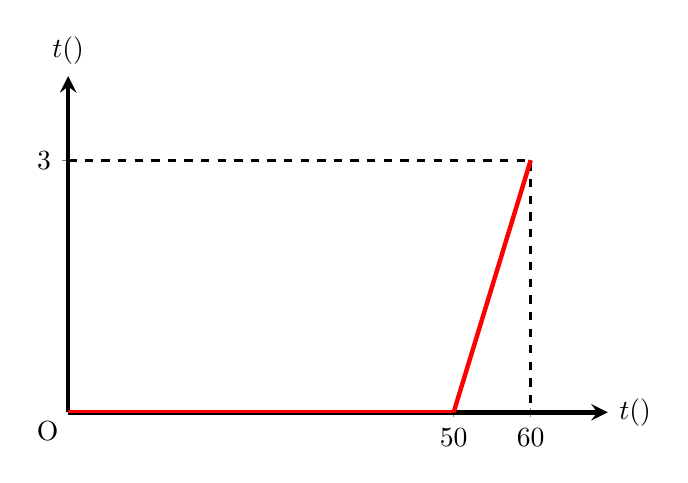
\begin{tikzpicture}  
			\begin{axis}[  ultra thick,yscale=0.75,
				xmin=0,  
				xmax=70,  
				xtick={0,50,60},
				ytick={0,3},
				ymin=0,  
				ymax=4, 
				samples=300,
				axis lines=center, 
				xlabel=$\xsi{t}{\left(\si{\minute}\right)}$, 		ylabel=$\xsi{t}{\left(\si{\celsius}\right)}$,
				every axis y label/.style={at=(current axis.above origin),anchor=south},  
				every axis x label/.style={at=(current axis.right of origin),anchor=west},  ]
				\draw[dashed, line width=1pt] (axis cs: 0,3)--++(axis cs: 60,0)--++(axis cs: 0,-3);
				\addplot [ultra thick, red, smooth, domain=0:50] {0};  
				\addplot [ultra thick, red, smooth, domain=50:60] {0.3*(x-50)} ;
				\coordinate (O) at (axis cs: 0,0) ;
				
			\end{axis}  
			\node[below left] at(O){O};
		\end{tikzpicture}
	\end{center}
	\choice
	{$\SI{5.54}{\kilogram}$}
	{\True $\SI{0.63}{\kilogram}$}
	{$\SI{0.54}{\kilogram}$}
	{$\SI{1.26}{\kilogram}$}
	\loigiai{
	Nhiệt lượng phòng tỏa ra trong khoảng thời gian từ $\SI{50}{\minute}$ đến $\SI{60}{\minute}$:
	$$Q=Mc\Delta t=\left(\SI{6.8}{\kilogram}\right)\cdot\left(\SI{4200}{\joule/\kilogram\cdot\kelvin}\right)\cdot\left(\SI{3}{\kelvin}\right)=\SI{85680}{\joule}$$
	Khối lượng nước đá trong hỗn hợp:
	$$m_{\text{đ}}=\dfrac{5Q}{\lambda}=\SI{1.26}{\kilogram}.$$
	Khối lượng nước đá còn lại ở thời điểm phút thứ 25:
	$$m'=\dfrac{m_{\text{đ}}}{2}=\SI{0.63}{\kilogram}.$$
	}
\end{ex}
% ===================================================================
\begin{ex}
	Có hai bình cách nhiệt: bình 1 chứa $\SI{2}{\kilogram}$ nước ở $\SI{20}{\celsius}$, bình 2 chứa $\SI{5}{\kilogram}$ nước ở $\SI{60}{\celsius}$. Ban đầu, người ta rót $\xsi{\Delta m}{\left(\kilogram\right)}$ nước từ bình 1 sang bình 2. Khi bình 2 cân bằng nhiệt, người ta lại rót $2\xsi{\Delta m}{\left(\kilogram\right)}$ nước từ bình 2 về bình 1. Khi bình 1 cân bằng nhiệt thì độ chênh lệch nhiệt độ giữa hai bình lúc này là $\SI{20}{\celsius}$. Giá trị của $\Delta m$ là
	\choice
	{$\SI{0.65}{\kilogram}$}
	{$\SI{0.45}{\kilogram}$}
	{\True $\SI{0.57}{\kilogram}$}
	{$\SI{0.35}{\kilogram}$}
	\loigiai{
	\textbf{* Khi rót $\Delta m$ từ bình 1 sang bình 2:}\\
	$$m_2c\left(t_{\text{cb2}}-t_2\right)+c\left(t_{\text{cb2}}-t_1\right)\Delta m=0\Rightarrow t_{\text{cb2}}=\dfrac{m_2t_2+t_1\Delta m}{m_2+\Delta m}=\dfrac{300+20\Delta m}{5+\Delta m}.$$
	\textbf{* Khi rót $2\Delta m$ từ bình 2 sang bình 1:}\\
	$$\left(m_1-\Delta m\right)c\left(t_{\text{cb1}}-t_1\right)+c\left(t_{\text{cb1}}-t_{\text{cb2}}\right)\cdot2\Delta m=0\Rightarrow t_{\text{cb1}}=\dfrac{2\left(t_{\text{cb2}}-t_{\text{cb1}}\right)\Delta m}{2-\Delta m}+20=\dfrac{40\Delta m}{2-\Delta m}+20$$
	Mà $t_{\text{cb2}}-t_{\text{cb1}}=20\Rightarrow \Delta m\approx\SI{0.57}{\kilogram}.$
	}
\end{ex}
\Closesolutionfile{ans}
\section{Câu trắc nghiệm đúng sai}
\textit{Thí sinh trả lời từ câu 1 đến câu 4. Trong mỗi ý \textbf{a)}, \textbf{b}, \textbf{c)}, \textbf{d)} ở mỗi câu, thí sinh chọn đúng hoặc sai}
\setcounter{ex}{0}
\Opensolutionfile{ans}[ans/Y24-VN12-PH-C1-TF]
% ===================================================================
\begin{ex}
	Xét cấu trúc của chất lỏng thì
	\choiceTF[t]
	{\True khoảng cách trung bình giữa các phân tử trong chất lỏng lớn hơn khoảng cách trung bình giữa các phân tử trong chất rắn và nhỏ hơn khoảng cách trung bình của các phân tử trong chất khí}
	{các phân tử chất lỏng dao động xung quanh vị trí cân bằng cố định}
	{\True chất lỏng có thể tích xác định nhưng không có hình dạng xác định mà hình dạng của nó phụ thuộc vào hình dạng của phần bình chứa nó}
	{\True lực tương tác giữa các phân tử ở thể lỏng lớn hơn lực tương tác giữa các phân tử ở thể khí}
	\loigiai{}
\end{ex}
% ===================================================================
\begin{ex}
	\immini{
		Máy thuỷ lực là một thiết bị quan trọng trong ngành xây dựng, kỹ thuật ô tô, \dots. Bên trong máy thuỷ lực người ta dùng một chất lỏng (dầu thuỷ lực). Khi ta tác dụng một lực $f$ lên piston nhỏ có diện tích $s$ lực này gây ra áp suất $p=f/s$ và được truyền nguyên vẹn đến piston lớn có diện tích $S$ và gây ra lực nâng $F$.	
	}
	{
		\includegraphics[width=0.6\linewidth]{../figs/Y24-VN12-PH-C1-BT-1}
	}
	\choiceTF[t]
	{Có thể thay thế chất lỏng trong máy thuỷ lực bằng chất khí}
	{Người ta sử dụng dầu thuỷ lực vì dầu thuỷ lực có đặc tính rất khó bị nén}
	{\True Nếu người ta nén với lực $f$ rất lón, các phân tử chất lỏng trong máy thuỷ lực càng bị nén chặt và có thể chuyển sang thể rắn}
	{Giả sử piston lớn có diện tích gấp 50 lần piston nhỏ. Khi đó, nếu muốn nâng một xe có khối lượng $\SI{1500}{\kilogram}$ thì cần tác dụng lên piston nhỏ một lực $\SI{30}{\newton}$}
	\loigiai{
		\begin{itemchoice}
			\itemch Sai. Vì chất khí dễ bị nén nên máy không hoạt động được.
			\itemch Đúng.
			\itemch Sai. Chất lỏng không thể chuyển thành thể rắn khi chỉ bị nén.
			\itemch Sai. $p=\dfrac{f}{s}=\dfrac{F}{S}\Rightarrow f=\dfrac{Fs}{S}=\SI{300}{\newton}$.
			
		\end{itemchoice}	
	}
\end{ex}
% ===================================================================
\begin{ex}
	Một khối băng có khối lượng $m =\SI{800}{\gram}$ ở $\SI{-10}{\celsius}$. Biết nhiệt dung riêng của nước đá là $c_{\text{đ}}= \SI{2090}{\joule/\kilogram\cdot\kelvin}$; nhiệt dung riêng của nước là $c_n =\SI{4190}{\joule/\kilogram\cdot\kelvin}$ và nhiệt nóng chảy riêng của nước đá $\lambda=\SI{3.33E5}{\joule/\kilogram}$.
	\choiceTF[t]
	{Để nóng chảy hoàn toàn, khối băng cần nhận được một năng lượng xấp xỉ $\SI{16720}{\joule}$}
	{Khi ở  $\SI{0}{\celsius}$, nếu truyền một nhiệt lượng $\SI{3352}{\joule}$ thì khối băng tan hoàn toàn thành nước ở nhiệt độ $\SI{0}{\celsius}$}
	{\True Khi băng bắt đầu nóng chảy, nếu nhận được nhiệt lượng $\SI{83.25}{\kilo\joule}$ thì khối lượng băng còn lại là $\SI{550}{\gram}$}
	{\True Cần một năng lượng $\SI{336.92}{\kilo\joule}$ truyền cho khối băng để nó chuyển hoàn toàn sang trạng thái lỏng ở $\SI{25}{\celsius}$}
	\loigiai{
	\begin{itemchoice}
		\itemch Sai. $Q=mc_{\text{đ}}\Delta t+m\lambda=\SI{283120}{\joule}$.
		\itemch Sai. $Q=m\lambda=\SI{266400}{\joule}$.
		\itemch Đúng.
		\itemch Đúng.
	\end{itemchoice}
	}
\end{ex}
% ===================================================================
\begin{ex}
	Người ta dùng một lò hồ quang điện để nấu chảy một khối kim loại nặng $\SI{29}{\kilogram}$. Biết mỗi phút lò hồ quang cung cấp cho khối kim loại một nhiệt lượng không đổi là $\SI{400}{\kilo\joule}$. Sự thay đổi nhiệt độ của khối kim loại được ghi lại theo thời gian như hình vẽ.
	\begin{center}
		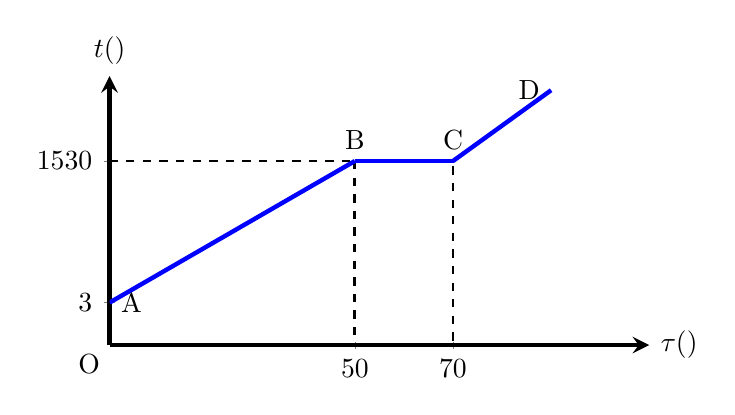
\begin{tikzpicture}  
			\begin{axis}[  ultra thick,yscale=0.6,
				xmin=0,  
				xmax=110,  
				xtick={0,50,70},
				ytick={0,3,13},
				yticklabels={0,3,1530},
				ymin=0,  
				ymax=19, 
				samples=300,
				axis lines=center, 
				xlabel=$\xsi{\tau}{\left(\si{\minute}\right)}$, 		ylabel=$\xsi{t}{\left(\si{\celsius}\right)}$,
				every axis y label/.style={at=(current axis.above origin),anchor=south},  
				every axis x label/.style={at=(current axis.right of origin),anchor=west},  ]
				\draw[dashed, line width=1pt] (axis cs: 0,13)--++(axis cs: 70,0)--++(axis cs: 0,-13);
				\draw[dashed, line width=1pt] (axis cs: 50,13)--(axis cs: 50,0);
				\addplot [ultra thick, blue, smooth, domain=0:50] {3+0.2*x};  
				\addplot [ultra thick, blue, smooth, domain=50:70] {13};
				\addplot [ultra thick, blue, smooth, domain=70:90] {13+0.25*(x-70)};
				\node[right] at (0,3) {A};
				\node[above] at (50,13) {B};
				\node[above] at (70,13) {C};
				\node[left] at (90,18) {D};
				\coordinate (O) at (axis cs: 0,0);
			\end{axis}  
			\node[below left] at (O) {O};
		\end{tikzpicture}
	\end{center}
	\choiceTF[t]
	{Giai đoạn AB trên đồ thị tương ứng với quá trình nóng chảy của kim loại}
	{Giai đoạn BC khối kim loại không nhận thêm nhiệt lượng từ lò nung}
	{\True Nhiệt dung riêng của khối kim loại xấp xỉ $\SI{459.8}{\joule/\kilogram\cdot\kelvin}$}
	{\True Nhiệt nóng chảy riêng của khối kim loại xấp xỉ $\SI{276E3}{\joule/\kilogram}$}
	\loigiai{
	\begin{itemchoice}
		\itemch Sai. Giai đoạn AB khối kim loại được nung nóng và đang tăng nhiệt độ.
		\itemch Sai. Khối kim loại vẫn nhận thêm nhiệt lượng và đang nóng chảy.
		\itemch Đúng.
		\itemch Đúng.
	\end{itemchoice}
	}
\end{ex}
\Closesolutionfile{ans}
\section{Câu trắc nghiệm trả lời ngắn} \textit{Thí sinh trả lời từ câu 1 đến câu 6}
\setcounter{ex}{0}
\Opensolutionfile{ans}[ans/Y24-VN12-PH-C1-TL]
% ===============================================================
\begin{ex}
Những viên nước đá ở $\SI{0}{\celsius}$ và khối lượng mỗi viên là $\SI{200}{\gram}$ lần lượt được thả vào $\SI{2}{\kilogram}$ nước ở $\SI{32}{\celsius}$ sao cho khi viên nước đá trước khi tan hết thì viên tiếp theo mới được thả vào. Cho biết năng lượng nhiệt cần thiết để làm tan $\SI{1}{\gram}$ nước đá  là $\SI{334}{\joule}$ và nhiệt dung riêng của nước là $\SI{4.18}{\joule/\left(\gram\cdot\kelvin\right)}$. Xác định số viên đá tối đa có thể thả vào lượng nước trên để trong nước không còn sót lại phần đá nào.	
	\shortans{4}
	\loigiai{
		Nhiệt lượng nước tỏa ra để giảm từ $\SI{32}{\celsius}$ xuống còn $\SI{0}{\celsius}$ có thể làm tan tối đa số viên đá là:
		$$N=\dfrac{m_nct_0}{\lambda m_\text{đ}}=4,005.$$
	}
\end{ex}
% ===============================================================
\begin{ex}
Biết rằng khoảng cách mỗi độ chia trong thang đo nhiệt độ X tương ứng với 1,5 độ chia trong thang đo nhiệt độ Y. Một vật khi có nhiệt độ $\SI{25}{\degree X}$ sẽ có nhiệt độ tương ứng là $\SI{45}{\degree Y}$ trong thang đo nhiệt độ Y. Khi nhiệt độ đo được ở thang Y là $\SI{50}{\degree Y}$ thì nhiệt độ tương ứng trong thang X là bao nhiêu $\si{\degree X}$?	
	\shortans{32,5 }
	\loigiai{
		$$\left(T_X-\SI{25}{\degree X}\right)\cdot1=\left(T_Y-\SI{45}{\degree Y}\right)\cdot 1,5\Rightarrow T_X=1,5T_Y-42,5$$
		Khi $T_Y=\SI{50}{\degree Y}$ thì $T_X=\SI{32.5}{\degree X}$.
	}
\end{ex}
% ===============================================================
\begin{ex}
Một khối khí được đặt trong một xilanh nằm ngang, được đậy kín bằng một pit-tông. Người ta cung cấp cho khối khí một nhiệt lượng $\SI{5}{\joule}$. Lúc này khối khí nở ra và đẩy pit-tông dịch chuyển (coi là chuyển động đều) một đoạn $\SI{10}{\centi\meter}$. Biết rằng lực ma sát giữa pit-tông và xilanh có độ lớn $F_{\text{ms}} =\SI{10}{\newton}$. Tính độ biến thiên nội năng của khối khí theo đơn vị $\si{\joule}$.	
	\shortans{4}
	\loigiai{
	Công do khối khí thực hiện:
	$$A'=Fs=\left(\SI{10}{\newton}\right)\cdot\left(\SI{0.1}{\meter}\right)=\SI{1}{\joule}.$$
	Độ biến thiên nội năng của khối khí:
	$$\Delta U=Q+A=Q-A'=\SI{4}{\joule}.$$	
	}
\end{ex}
% ===============================================================
\begin{ex}
	Một người cọ xát một miếng sắt dẹt có khối lượng $\SI{150}{\gram}$ trên một tấm đá mài. Sau một khoảng thời gian, miếng sắt nóng thêm $\SI{12}{\celsius}$. Giả sử rằng $\SI{40}{\percent}$ công đó được dùng để làm nóng miếng sắt. Biết nhiệt dung riêng của sắt là $\SI{460}{\joule/\kilogram\cdot\kelvin}$. Công mà người này đã thực hiện là bao nhiêu $\si{\joule}$?
	\shortans{2070 }
	\loigiai{
		$A=\dfrac{mc\Delta t}{H}=\SI{2070}{\joule}.$
	}
\end{ex}
% ===============================================================
\begin{ex}
Trong thí nghiệm đo nhiệt dung riêng của nước, công suất điện trên oát kế là $\SI{950}{\watt}$, khối lượng nước được sử dụng là $\SI{1}{\kilogram}$. Đồ thị thực nghiệm nhiệt độ phụ thuộc vào thời gian xác định được như hình bên dưới.
\begin{center}
	\includegraphics[width=0.7\linewidth]{../figs/Y24-VN12-PH-C1-BT-2}
\end{center}	
Hãy tính nhiệt dung riêng của nước ra đơn vị J/kg.K.
	\shortans{ 4256}
	\loigiai{
		$$c=\dfrac{\calP t}{m\Delta t}=\dfrac{\left(\SI{950}{\watt}\right)\cdot\left(\SI{144}{\second}-\SI{32}{\second}\right)}{\left(\SI{1}{\kilogram}\right)\cdot\left(\SI{60}{\celsius}-\SI{35}{\celsius}\right)}=\SI{4256}{\joule/\kilogram\cdot\kelvin}.$$
	}
\end{ex}
% ===============================================================
\begin{ex}
Có ba bình nước giống nhau, mỗi bình chứa $\SI{20}{\gram}$ nước ở cùng nhiệt độ. Người ta thả vào mỗi bình một cục nước đá có khối lượng khác nhau nhưng có cùng nhiệt độ. Bình 1 được thả cục nước đá có khối lượng $\SI{10}{\gram}$, khi cân bằng nhiệt, khối lượng nước đá còn lại trong bình là $\SI{9}{\gram}$. Bình 2 được thả cục nước đá có khối lượng $\SI{20}{\gram}$, khi cân bằng nhiệt, khối lượng nước đá trong bình không đổi. Bình 3 được thả cục nước đá có khối lượng $\SI{40}{\gram}$, khi có cân bằng nhiệt, khối lượng nước đá trong bình là bao nhiêu gram?	
	\shortans{42 }
	\loigiai{
		Bình 1 chỉ có $\Delta m_1=\SI{1}{\gram}$ đá tan thành nước $\Rightarrow$ nhiệt độ cân bằng của hỗn hợp là $\SI{0}{\celsius}$:
		$$m_nc_nt_n=m_{\text{đ1}}c\left(0-t_{\text{đ}}\right)+\lambda\Delta m_1$$
		\begin{equation}
			\Rightarrow 20c_nt_n=-10ct_{\text{đ}}+\lambda
			\label{eq: 1}
		\end{equation}
		Bình 2 có khối lượng nước đá không đổi, chứng tỏ nhiệt lượng nước tỏa ra để giảm nhiệt độ xuống $\SI{0}{\celsius}$ bằng nhiệt lượng nước đá thu vào để tăng nhiệt độ lên $\SI{0}{\celsius}$.
		\begin{equation}
			m_nc_nt_n=-m_{\text{đ2}}ct_{\text{đ}}
			\Leftrightarrow c_nt_n=-c_\text{đ}t_{\text{đ}}
			\label{eq: 2}
		\end{equation}
		Từ \eqref{eq: 1} và \eqref{eq: 2}, suy ra:
		$$\begin{cases}
		c_nt_n=0,1\lambda\\
			ct_{\text{đ}}=-0,1\lambda
		\end{cases}$$
		Bình 3 được thả cục nước đá có khối lượng $\SI{40}{\gram}$ nên nước sẽ bị đóng băng, khối lượng nước đóng băng là $m_{\text{b}}$:
		$$m_nc_nt_n+m_b\lambda=-m_{\text{đ3}}ct_{\text{đ}}\Leftrightarrow 20\cdot0,1\lambda+m_b\lambda=40\cdot0,1\lambda\Rightarrow m_{\text{b}}=\SI{2}{\gram}.$$
		Vậy bình 3 khi cân bằng nhiệt thì khối lượng nước đá là $m_{\text{đ3}}+m_{\text{b}}=\SI{42}{\gram}.$
	}
\end{ex}
\Closesolutionfile{ans}


%	\stopcontents[mychapters]
%		\mychapter{KHÍ LÍ TƯỞNG}
%	\startcontents[mychapters]
%	\printcontents[mychapters]{}{0}{\setcounter{tocdepth}{1}}
%	\begin{center}
%			\includegraphics[width=0.7\linewidth]{../figs/G12C2}
%		\end{center}
%	\chapter{Tóm tắt lý thuyết}
\section{Mô hình động học phân tử chất khí}
\subsection{Chuyển động Brown}
\begin{itemize}
	\item Chuyển động Brown là chuyển động hỗn loạn, không ngừng, không theo quy luật, có quỹ đạo là đường gấp khúc bất kì của các hạt nhẹ trong chất lỏng và chất khí.
	\item Chuyển động Brown chứng tỏ các phân tử khí chuyển động hỗn loạn, không ngừng.
	\item Nhiệt độ càng cao, các phân tử khí chuyển động càng nhanh.
\end{itemize}
\subsection{Thuyết động học phân tử chất khí}
\begin{itemize}
	\item Chất khí được cấu tạo từ các phân tử có kích thước rất nhỏ so với khoảng cách trung bình giữa chúng.
	\item Các phân tử khí luôn chuyển động hỗn loạn, không ngừng. Nhiệt độ càng cao, các phân tử khí chuyển động càng nhanh.
	\item Trong quá trình chuyển động, các phân tử khí va chạm với thành bình chứa, gây ra áp suất lên thành bình.
\end{itemize}
\subsection{Lượng chất}
\begin{itemize}
	\item Đơn vị đo lượng chất là $\si{\mole}$.
	\item Mol là lượng chất trong đó chứa số phân tử (hoặc nguyên tử) bằng $N_A = \SI{6.022E23}{\mole^{-1}}$.	$N_A$ được gọi là số Avogadro.
	\item Một mẫu chất có khối lượng $m$, chứa $N$ phân tử thì có số mol là: $n=\dfrac{N}{N_A}=\dfrac{m}{M}$, trong đó
	$M$ (khối lượng mol) là khối lượng của 1 mol chất đó.
\end{itemize}
\section{Các định luật khí lí tưởng}
\subsection{Khí lí tưởng}
\begin{itemize}
	\item Khí lí tưởng là chất khí tuân theo đúng định luật Boyle và định luật Charles.
	\item Nội năng của khí lí tưởng chỉ phụ thuộc vào nhiệt độ.
\end{itemize}
\subsection{Định luật Boyle}
\begin{itemize}
	\item Ở nhiệt độ không đổi, áp suất của một khối lượng khí xác định tỉ lệ nghịch với thể tích	của nó.
	$$pV=\text{hằng số}\quad \text{hay}\quad p_1V_1=p_2$$
	\item Đồ thị biểu diễn sự phụ thuộc của áp suất theo thể tích khi nhiệt độ của khối khí không đổi được gọi là đường đẳng nhiệt.
	\begin{center}
		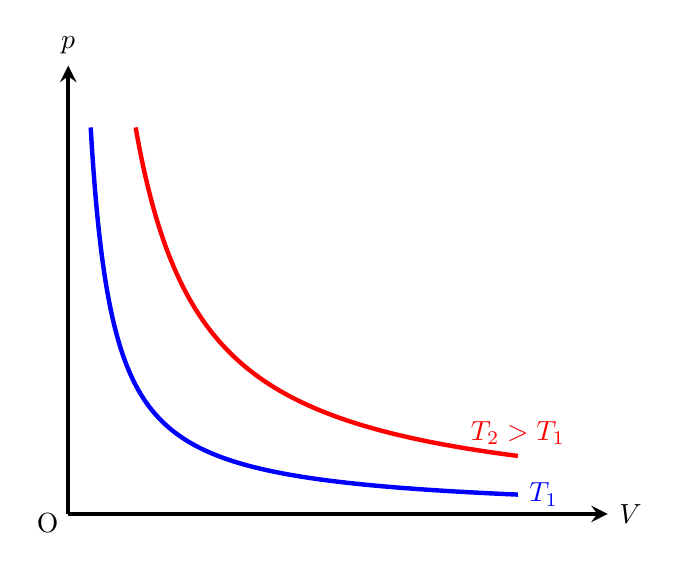
\begin{tikzpicture}  
			\begin{axis}[  ultra thick,
				xmin=0,  
				xmax=24,  
				xtick=\empty,
				ytick=\empty,
				ymin=0,  
				ymax=5.8, 
				samples=300,
				xticklabels=\empty,
				yticklabels=\empty,
				axis lines=center, 
				xlabel=$V$, 
				ylabel=$p$, 
				every axis y label/.style={at=(current axis.above origin),anchor=south},  
				every axis x label/.style={at=(current axis.right of origin),anchor=west},  ]
				\addplot [ultra thick, blue, smooth, domain=1:20] {5/x} node[right] {$T_1$}; 
				\addplot [ultra thick, red, smooth, domain=3:20] {15/x} node[above] {$T_2>T_1$}; 
			\end{axis}  
			\node[label={[below left]90:O}] at (0,0){};
		\end{tikzpicture}
	\end{center}
\end{itemize}
\subsection{Định luật Charles}
\begin{itemize}
	\item Ở áp suất không đổi, thể tích của một khối lượng khí xác định tỉ lệ thuận với nhiệt độ tuyệt đối của nó.
	$$\dfrac{V}{T}=\text{hằng số}\quad \text{hay}\quad \dfrac{V_1}{T_1}=\dfrac{V_2}{T_2}$$
	\item Đồ thị biểu diễn sự phụ thuộc của thể tích theo nhiệt độ tuyệt đối khi áp suất của khối khí không đổi được gọi là đường đẳng áp.
	\begin{center}
		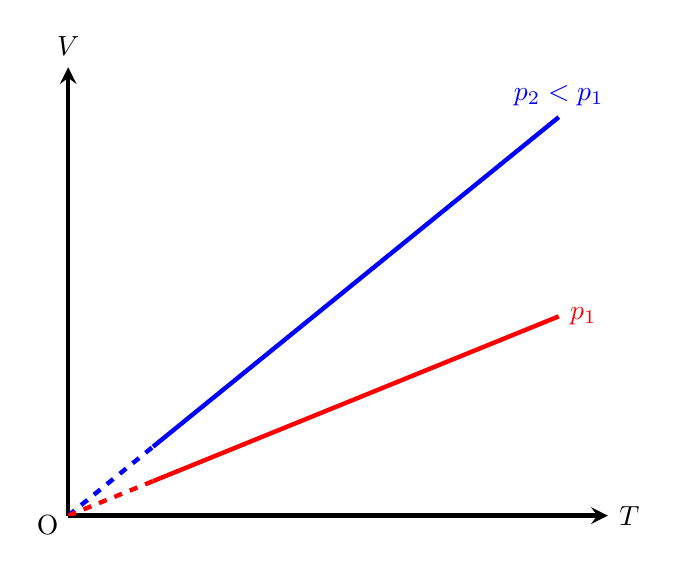
\begin{tikzpicture}  
			\begin{axis}[  ultra thick,
				xmin=0,  
				xmax=1100,  
				xtick=\empty,
				ytick=\empty,
				ymin=0,  
				ymax=900, 
				samples=300,
				xticklabels=\empty,
				yticklabels=\empty,
				axis lines=center, 
				xlabel=$T$, 
				ylabel=$V$, 
				every axis y label/.style={at=(current axis.above origin),anchor=south},  
				every axis x label/.style={at=(current axis.right of origin),anchor=west},  ]
				\addplot [ultra thick, blue, smooth,dashed, domain=0:173] {0.8*x}; 
				\addplot [ultra thick, blue, smooth, domain=173:1000] {0.8*x} node[above]{$p_2<p_1$}; 
				\addplot [ultra thick, red, smooth,dashed, domain=0:173] {0.4*x}; 
				\addplot [ultra thick, red, smooth, domain=173:1000] {0.4*x} node[right]{$p_1$};
			\end{axis}  
			\node[label={[below left]90:O}] at (0,0){};
		\end{tikzpicture}
	\end{center}
\end{itemize}
\subsection{Phương trình trạng thái của khí lí tưởng}
$$\dfrac{pV}{T}=nR\quad \text{hay}\quad \dfrac{p_1V_1}{T_1}=\dfrac{p_2V_2}{T_2}$$
Trong đó, $R\approx \SI{8.31}{\joule/\mole\cdot\kelvin} \approx\SI{0.082}{\dfrac{\liter\cdot atm}{\mole\cdot\kelvin}}$
là hằng số khí lí tưởng; $n$ là số mol khí.
\section{Áp suất và động năng của phân tử khí}
\subsection{Áp suất chất khí}
\begin{itemize}
	\item Áp suất khí tác dụng lên thành bình càng tăng khi các phân tử khí chuyển động nhiệt càng nhanh, khối lượng và mật độ phân tử khí càng lớn.
	\item Biểu thức tính áp suất chất khí tác dụng lên thành bình:
\end{itemize}
$$p=\dfrac{1}{3}\mu m\overline{v^2}=\dfrac{2}{3}\mu W_{\text{đ}}$$
trong đó:
\begin{itemize}
	\item $p$: áp suất khí tác dụng lên thành bình, đơn vị trong hệ SI là $\si{\newton/\meter^2}$;
	\item $\mu=\dfrac{N}{V}$: mật độ phân tử khí, đơn vị trong hệ SI là $\si{\meter^{-3}}$;
	\item $m$: khối lượng của một phân tử khí, đơn vị trong hệ SI là $\si{\kilogram}$;
	\item $\overline{v^2}$: trung bình của bình phương tốc độ, đơn vị trong hệ SI là $\si{\meter^2/\second^2}$;
	\item $W_{\text{đ}}$: động năng tịnh tiến trung bình của phân tử, đơn vị trong hệ SI là $\si{\joule}$.
\end{itemize}
\luuy{
Tốc độ căn quân phương $v_c=\sqrt{\overline{v^2}}$ \textbf{không phải} là tốc độ trung bình của các phân tử khí.
}
\subsection{Động năng tịnh tiến trung bình của phân tử khí}
Động năng tịnh tiến trung bình của phân tử khí tỉ lệ thuận với nhiệt độ tuyệt đối của khí.
$$W_{\text{đ}}=\dfrac{3}{2}kT.$$
Trong đó $k$ là hằng số Boltzmann: $k=\dfrac{R}{N_A}\approx\SI{1.38E-23}{\joule/\kelvin}$.
\subsection{Nội năng của khí lí tưởng đơn nguyên tử}
$$U=\dfrac{3}{2}nRT.$$
%	\chapter{Câu hỏi ôn tập}
\hideall{
\setcounter{section}{0}
\begin{center}
	\textbf{\large BẢNG ĐÁP ÁN}
\end{center}
\section{Câu trắc nghiệm nhiều phương án lựa chọn}
\inputansbox{10}{ans/Y24-VN12-PH-C2-TN}
\section{Câu trắc nghiệm đúng sai}
\inputansbox[2]{2}{ans/Y24-VN12-PH-C2-TF}
\section{Câu trắc nghiệm trả lời ngắn}
\inputansbox[3]{6}{ans/Y24-VN12-PH-C2-TL}
}
\setcounter{section}{0}
\section{Câu trắc nghiệm nhiều phương án lựa chọn}
\textit{Thí sinh trả lời từ câu 1 đến câu 18. Mỗi câu thí sinh chọn một phương án}
\setcounter{ex}{0}
\Opensolutionfile{ans}[ans/Y24-VN12-PH-C2-TN]
% ===================================================================
\begin{ex}
	Khi nhiệt độ của một khối khí lý tưởng tăng ở áp suất không đổi, khối lượng riêng của khối khí sẽ như thế nào?
	\choice
	{\True Khối lượng riêng giảm}
	{Khối lượng riêng không thay đổi}
	{Khối lượng riêng có thể tăng hoặc giảm}
	{Khối lượng riêng tăng}
	\loigiai{}
\end{ex}
% ===================================================================
\begin{ex}
	Thiết bị nào sau đây không dùng để xác định nhiệt hoá hơi riêng của nước?
	\choice
	{Oát kế}
	{Cân điện tử}
	{Nhiệt lượng kế}
	{\True Nhiệt kế}
	\loigiai{}
\end{ex}
% ===================================================================
\begin{ex}
	Bơm căng săm xe đạp và vặn van thật chặt nhưng để lâu ngày vẫn bị xẹp lốp vì
	\choice
	{săm xe làm bằng cao su là chất đàn hồi, nên sau khi giãn ra thì tự động co lại làm cho săm để lâu ngày bị xẹp}
	{lúc bơm, không khí vào săm còn nóng, sau đó không khí nguội dần, co lại, làm săm xe bị xẹp}
	{\True giữa các phân tử cao su dùng làm săm có khoảng cách nên các phân tử không khí có thể thoát ra ngoài làm săm xẹp dần}
	{cao su dùng làm săm đẩy các phân tử không khí lại gần nhau nên săm bị xẹp}
	\loigiai{}
\end{ex}
% ===================================================================
\begin{ex}
	 Quần áo khô sau khi phơi dưới ánh nắng mặt trời. Hiện tượng này thể hiện?
	\choice
	{\True Sự bay hơi của nước}
	{Sự nóng chảy của nước}
	{Sự đông đặc của nước}
	{Sự ngưng tụ của nước}
	\loigiai{}
\end{ex}
% ===================================================================
\begin{ex}
Người ta ghi chép rằng tại cửa sông Amazon đã tìm thấy một thỏi vàng thiên nhiên có khối lượng $\SI{62.3}{\kilogram}$. Nếu khối lượng mol của vàng là $\SI{197}{\gram/\mole}$ thì số mol của thỏi vàng này gần giá trị nào nhất sau đây?	
	\choice
	{\SI{132}{\mole}}
	{\SI{457}{\mole}}
	{\SI{477}{\mole}}
	{\True \SI{316}{\mole}}
	\loigiai{}
\end{ex}
% ===================================================================
\begin{ex}
	Công thức nào sau đây là công thức tổng quát của định luật một nhiệt động lực học?
	\choice
	{$\Delta U=Q$}
	{\True $\Delta U=Q+A$}
	{$\Delta U=A$}
	{$A+Q=0$}
	\loigiai{}
\end{ex}
% ===================================================================
\begin{ex}
	Khi dùng các đèn cồn giống hệt nhau để đun các bình nước khác nhau trong cùng một khoảng thời gian, người ta thấy nhiệt độ trong các bình là khác nhau. Yếu tố nào sau đây làm cho nhiệt độ của nước ở trong các bình trở nên khác nhau khi ta đun nước?
	\choice
	{Thời gian đun}
	{Nhiệt lượng mà các bình nhận được}
	{\True Lượng chất lỏng chứa trong từng bình}
	{Loại chất lỏng chứa trong từng bình}
	\loigiai{}
\end{ex}
% ===================================================================
\begin{ex}
	Tính chất nào sau đây \textbf{không phải} của phân tử vật chất ở thể khí?
	\choice
	{chuyển động không ngừng}
	{chuyển động hỗn loạn}
	{chuyển động hỗn loạn và không ngừng}
	{\True chuyển động hỗn loạn xung quanh các vị trí cân bằng cố định}
	\loigiai{}
\end{ex}
% ===================================================================
\begin{ex}
	Một bọt khí nổi lên từ một đáy hồ nước. Khi đến mặt nước, nó có thể tích gấp 1,2 lần ban đầu. Coi nhiệt độ của bọt khí là không đổi. So với áp suất trên mặt hồ thì áp suất dưới đáy hồ
	\choice
	{lớn hơn 1,44 lần}
	{nhỏ hơn 1,2 lần}
	{nhỏ hơn 2,4 lần}
	{\True lớn hơn 1,2 lần}
	\loigiai{}
\end{ex}
% ===================================================================
\begin{ex}
	Gọi $p$ là áp suất, $V$ là thể tích, $R$ là hằng số khí lí tưởng, $k$ là hằng số Boltzmann và $T$ là nhiệt độ tuyệt đối. Số mol khí có trong một khối lượng chất khí cho trước được xác định bởi biểu thức
	\choice
	{$\dfrac{pR}{VT}$}
	{$\dfrac{pV}{kT}$}
	{\True $\dfrac{pV}{RT}$}
	{$pV$}
	\loigiai{}
\end{ex}
% ===================================================================
\begin{ex}
	Biết nhiệt nóng chảy riêng của nước đá là $\lambda=\SI{3.4E5}{\joule/\kilogram}$. Nhiệt lượng $Q$ cần cung cấp để làm nóng chảy hoàn toàn $\SI{100}{\gram}$ nước đá ở $\SI{0}{\celsius}$ bằng
	\choice
	{$\SI{340E5}{\joule}$}
	{$\SI{0.34E3}{\joule}$}
	{$\SI{34E7}{\joule}$}
	{\True $\SI{34E3}{\joule}$}
	\loigiai{}
\end{ex}
% ===================================================================
\begin{ex}
	Phát biểu nào sau đây về nội năng là không đúng?
	\choice
	{Nội năng là một dạng năng lượng}
	{Nội năng có thể chuyển hoá thành các dạng năng lượng khác}
	{\True Nội năng là nhiệt lượng}
	{Nội năng của một vật có thể tăng lên, giảm đi}
	\loigiai{}
\end{ex}
% ===================================================================
\begin{ex}
	Nhiệt độ mùa đông tại thành phố NewYork (Mĩ) là $\SI{23}{\degree F}$. Ứng với nhiệt Celsius, nhiệt độ đó là
	\choice
	{\SI{10}{\celsius}}
	{\SI{-10}{\celsius}}
	{\SI{5}{\celsius}}
	{\True \SI{-5}{\celsius}}
	\loigiai{}
\end{ex}
% ===================================================================
\begin{ex}
	Bảng bên dưới cho biết nhiệt độ nóng chảy và nhiệt độ sôi của bốn chất.
\begin{center}
		\begin{tabular}{|M{5cm}|M{5cm}|M{5cm}|}
		\hline 
		\thead{Chất} & \thead{Nhiệt độ nóng chảy $\left(\si{\celsius}\right)$} & \thead{Nhiệt độ sôi $\left(\si{\celsius}\right)$} \\
		\hline 1 & $-210$ & $-196$ \\
		\hline 2 & $-39$ & 357 \\
		\hline 3 & 30 & 2400 \\
		\hline 4 & 327 & 1749 \\
		\hline
	\end{tabular}
\end{center}
	\choice
	{Chất 1}
	{\True Chất 2}
	{Chất 3}
	{Chất 4}
	\loigiai{}
\end{ex}
% ===================================================================
\begin{ex}
	\immini{Một khối khí thực hiện các quá trình biến đổi trạng thái như hình bên. Ý nào sau đây là \textbf{không đúng}?
		\choice
		{\True AB là quá trình nén đẳng tích}
		{$\dfrac{V_{\mathrm{A}}}{T_{\mathrm{A}}}=\dfrac{V_{\mathrm{B}}}{T_{\mathrm{B}}}$}
		{CA là quá trình dãn nở đẳng nhiệt}
		{$p_{\mathrm{A}}V_{\mathrm{A}}=p_{\mathrm{C}}V_{\mathrm{C}}$}}
		{\includegraphics[scale=0.5]{../figs/Y24-VN12-PH-C2-BT-1}}
	\loigiai{}
\end{ex}
% ===================================================================
\begin{ex}
	Một nhiệt kế có phạm vi đo từ $\SI{263}{\kelvin}$ đến $\SI{1273}{\kelvin}$, dùng để đo nhiệt độ của các lò nung. Phạm vi đo của nhiệt kế này trong thang nhiệt độ Celsius là
	\choice
	{\SI{-12}{\celsius} và \SI{1000}{\celsius}}
	{\SI{-20}{\celsius} và \SI{1200}{\celsius}}
	{\SI{0}{\celsius} và \SI{273}{\celsius}}
	{\True \SI{-10}{\celsius} và \SI{1000}{\celsius}}
	\loigiai{}
\end{ex}
% ===================================================================
\begin{ex}
	Một học sinh sử dụng bộ thiết bị như hình a) bên dưới để so sánh năng lượng nhiệt cần thiết để làm nóng những khối vật liệu khác nhau. Mỗi khối có khối lượng bằng nhau và có nhiệt độ ban đầu là \SI{20}{\celsius}. Học sinh đó tiến hành đo thời gian cần thiết để nhiệt độ của mỗi khối vật liệu tăng lên thêm \SI{5}{\celsius}. Kết quả được biểu diễn trên hình b) bên dưới. Vật liệu nào có nhiệt dung riêng lớn nhất?
	\begin{center}
		\includegraphics[scale=0.8]{../figs/Y24-VN12-PH-C2-BT-2}
	\end{center}
	\choice
	{\True Bê tông}
	{Thiếc}
	{Sắt}
	{Đồng}
	\loigiai{}
\end{ex}
% ===================================================================
\begin{ex}
	\immini{Trên đồ thị $\left(V, T\right)$ (xem hình vẽ bên) vẽ bốn đường đẳng áp của cùng một lượng khí. Đường ứng với áp suất thấp nhất là
		\choice
		{\True $p_4$}
		{$p_1$}
		{$p_3$}
		{$p_2$}}
		{\vspace{-0.75cm}\includegraphics[scale=0.7]{../figs/Y24-VN12-PH-C2-BT-3}}
	\loigiai{}
\end{ex}
\Closesolutionfile{ans}
\section{Câu trắc nghiệm đúng sai}
\textit{Thí sinh trả lời từ câu 1 đến câu 4. Trong mỗi ý \textbf{a)}, \textbf{b}, \textbf{c)}, \textbf{d)} ở mỗi câu, thí sinh chọn đúng hoặc sai}
\setcounter{ex}{0}
\Opensolutionfile{ans}[ans/Y24-VN12-PH-C2-TF]
% ===================================================================
\begin{ex}
	\immini{Một nhóm học sinh tìm hiểu về mối liên hệ giữa áp suất và thể tích của một lượng khí xác định khi nhiệt độ được giữ không đổi. Họ đã thực hiện các nội dung sau: Chuẩn bị bộ thí nghiệm (hình bên) dịch chuyển từ từ pit tông để làm thay đổi thể tích của khí, đọc và ghi kết quả áp suất, thể tích theo số chỉ của dụng cụ đo kết quả như bảng bên}
	{\vspace{-0.75cm}\includegraphics[scale=0.5]{../figs/Y24-VN12-PH-C2-BT-4}}
	\choiceTF[t]
	{Khi tiến hành thí nghiệm nhóm đã dịch chuyển từ từ pit tông để mục đích chính là giúp toàn thể các bạn trong nhóm có thời gian để nhìn rõ kết quả thay đổi các thông số của khí}
	{Bỏ qua sai số coi công thức liên hệ áp suất theo thể tích là $p=\dfrac{23}{V}$, $p$ đo bằng bar $\left(\SI{1}{bar}=\SI{E5}{\pascal}\right)$, $V$ đo bằng $\si{\centi\meter^3}$. Thể tích khí đã dùng trong thí nghiệm ở điều kiện tiêu chuẩn là 0,18 lít}
	{\True Số liệu thí nghiệm cho thấy áp suất tỉ lệ nghịch với thể tích của nó}
	{\True Thí nghiệm này đã kiểm chứng được định luật Boyle}
	\loigiai{}
\end{ex}
% ===================================================================
\begin{ex}
	\immini{Ngày 26 tháng 10 năm 2024 đã diễn ra lễ hội khinh khí cầu Tràng An - Cúc Phương năm 2024 tại Ninh Bình. Một khí cầu có thể tích $V=\SI{336}{\meter^3}$ và khối lượng vỏ $m=\SI{82}{\kilogram}$ được bơm không khí nóng tới áp suất bằng áp suất không khí bên ngoài. Biết không khí bên ngoài có nhiệt độ $\SI{30}{\celsius}$ và áp suất $\SI{1}{atm}$ (với $\SI{1}{atm}=\SI{101325}{\pascal}$); khối lượng mol của không khí ở điều kiện chuẩn là $\SI{29E-3}{\kilogram/\mole}$.}
	{\includegraphics[scale=0.1]{../figs/Y24-VN12-PH-C2-BT-5}}
	\choiceTF[t]
	{\True Nhiệt độ của không khí bên ngoài khí cầu là $\SI{303}{\kelvin}$}
	{\True Khối lượng riêng của không khí ở nhiệt độ $\SI{30}{\celsius}$ và áp suất \SI{1}{atm} là $\SI{1.17}{\gram/\liter}$}
	{\True Cho rằng lực của gió không đáng kể, lực chính đẩy khí cầu bay lên là lực Archimedes tác dụng vào khí cầu}
	{Cho rằng lực của gió không đáng kể để khí cầu bắt đầu bay lên thì nhiệt độ không khí nóng bên trong khí cầu là $\SI{368}{\kelvin}$}
	\loigiai{\begin{itemchoice}
			\itemch Đúng. $T=t+273=\SI{303}{\kelvin}$.
			\itemch Đúng. $\dfrac{p_0}{D_0T_0}=\dfrac{R}{M}\Leftrightarrow \dfrac{101325}{D_0\left(30+273\right)}=\dfrac{8,31}{\SI{29E-3}{}}\Rightarrow D_0\approx\SI{1.167}{\kilogram/\meter^3}=\SI{1.17}{\gram/\liter}$.
			\itemch Đúng. 
			\itemch Sai. \\
			$F_A=P\Rightarrow D_0gV=mg+DgV
			\Rightarrow 1,167\cdot336=82+D\cdot336\Rightarrow D\approx\SI{0.923}{\kilogram/\meter^3}$\\
			$\dfrac{p}{DT}=\dfrac{R}{M}\Rightarrow\dfrac{101325}{0,923\cdot T}=\dfrac{8,31}{\SI{29E-3}{}}\Rightarrow T\approx\SI{383}{\kelvin}$.
	\end{itemchoice}}
\end{ex}
% ===================================================================
\begin{ex}
\immini{	Một nhóm học sinh tìm hiểu về sự truyền nhiệt. Họ có các dụng cụ và cách tiến hành như sau: \\
	\textbf{Dụng cụ}\\
	\begin{itemize}
		\item Cốc nhôm đựng $\SI{200}{\milli\liter}$ nước ở nhiệt độ \SI{30}{\celsius} (1).
		\item Bình cách nhiệt đựng \SI{500}{\milli\liter} nước ở nhiệt độ \SI{60}{\celsius} (2).
		\item Hai nhiệt kế (3).
	\end{itemize}
	\textbf{Tiến hành}
	}
	{\includegraphics[scale=0.6]{../figs/Y24-VN12-PH-C2-BT-6}}
	\vspace{0.5cm}
\begin{itemize}
	\item Đặt cốc nhôm vào trong lòng bình cách nhiệt như hình vẽ và quan sát số chỉ nhiệt kế để tìm hiểu về sự truyền nhiệt của chúng.
\end{itemize}
	\choiceTF[t]
	{\True Nhiệt độ nước ở bình (2) giảm dần chứng tỏ nó thực hiện truyền nhiệt lượng}
	{\True Nhiệt độ nước trong cốc nhôm (1) tăng dần chứng tỏ nước trong cốc (1) được nhận nhiệt lượng}
	{Sau một thời gian cả hai nhiệt kế chỉ giá trị không đổi và bằng nhau chứng tỏ sự truyền nhiệt năng đã dừng lại khi nước trong hai bình tràn vào nhau có thể tích bằng nhau}
	{Thí nghiệm này có thể kiểm chứng cho kết luận: nhiệt năng truyền từ vật có khối lượng lớn hơn sang vật có khối lượng nhỏ hơn}
	\loigiai{}
\end{ex}
% ===================================================================
\begin{ex}
	\immini{Một học sinh tiến hành đun một khối nước đá đựng trong nhiệt lượng kế từ \SI{0}{\celsius} đến khi tan chảy hết thành nước và hóa hơi ở \SI{100}{\celsius}. Hình bên là đồ thị biểu diễn sự phụ thuộc của nhiệt lượng mà khối nước đá nhận được từ lúc đun đến lúc bay hơi và sự thay đổi nhiệt độ của nó. Lấy nhiệt nóng chảy riêng của nước đá là \SI{3.3E5}{\joule/\kilogram} và nhiệt dung riêng của nước đá là \SI{4200}{\joule/\kilogram},
		nhiệt hóa hơi riêng của nước là \SI{2.3E6}{\joule/\kilogram}, bỏ qua nhiệt dung của nhiệt lượng kế.}
		{\includegraphics[scale=0.8]{../figs/Y24-VN12-PH-C2-BT-7}}
	\choiceTF[t]
	{\True Tại điểm B trên đồ thị, nước bắt đầu xảy ra sự sôi}
	{\True Trong đoạn BC trên đồ thị, khối nước nhận nhiệt lượng để thực hiện quá trình hóa hơi}
	{\True Tại điểm C lượng nước còn lại là \SI{96}{\gram}}
	{Nếu tiến hành đun đến khi lượng nước bay hơi hết cần cung cấp nhiệt lượng tổng cộng là \SI{325}{\kilo\joule}}
	\loigiai{\begin{itemchoice}
			\itemch Đúng. 
			\itemch Đúng. 
			\itemch Đúng. $Q_B=m\left(\lambda+c\Delta t\right)\Leftrightarrow 90\cdot10^3=m\left(\SI{3.3E5}{}+4200\cdot100\right)\Rightarrow m=\SI{0.12}{\kilogram}$.\\
			$m_{\mathrm{BC}}=\dfrac{Q_C-Q_B}{L}=\SI{0.024}{\kilogram}$.\\
			Tại điểm C lượng nước còn lại là $m-m_{\mathrm{BC}}=0,12-0,024=\SI{0.096}{\kilogram}=\SI{96}{\gram}$.
			\itemch Sai. $Q_B+mL=90\cdot10^3+0,12\cdot2,3\cdot10^6=\SI{366}{\kilo\joule}$.
	\end{itemchoice}}
\end{ex}
\Closesolutionfile{ans}
\section{Câu trắc nghiệm trả lời ngắn} \textit{Thí sinh trả lời từ câu 1 đến câu 6}
\setcounter{ex}{0}
\Opensolutionfile{ans}[ans/Y24-VN12-PH-C2-TL]
% ===============================================================
\begin{ex}
	Một săm xe máy được bơm không khí ở \SI{27}{\celsius} tới áp suất \SI{2}{atm}. Săm chỉ có thể chịu được áp suất tối đa bằng \SI{3.0}{atm}. Bỏ qua sự nở nhiệt của săm. Nhiệt độ của không khí trong săm có thể có giá trị lớn nhất bằng bao nhiêu $\si{\celsius}$ để săm không bị nổ? (làm tròn kết quả đến chữ số hàng đơn vị).
	\shortans[oly]{177}
	\loigiai{
		$\dfrac{p}{T}=const\Rightarrow \dfrac{2}{27+273}=\dfrac{3}{T}\Rightarrow T=\SI{450}{\kelvin}\approx\SI{177}{\celsius}$.
	}
\end{ex}
% ===============================================================
\begin{ex}
Một bình đựng \SI{2.5}{\gram} khí helium có thể tích 5 lít và nhiệt độ ở \SI{27}{\celsius}. Áp suất khí trong bình là $\xsi{x\cdot10^5}{\newton/\meter^2}$. Giá trị của $x$ bằng bao nhiêu? (kết quả lấy 1 chữ số sau dấu phẩy thập phân).	
	\shortans[oly]{3,1}
	\loigiai{
	$pV=\dfrac{m}{M}RT\Rightarrow p\approx\SI{3.1e5}{\pascal}$.	
	}
\end{ex}
% ===============================================================
\begin{ex}
	\immini{Khi thở ra, dung tích của phổi là $\SI{2,400}{\liter}$ và áp suất của không khí trong phổi là \SI{101,70E3}{\pascal}. Cho biết khi hít vào, áp suất này trở thành \SI{101,12E3}{\pascal}. Dung tích của phổi khi hít vào là bao nhiêu lít? (kết quả lấy 2 chữ số sau dấu phẩy thập phân).}
	{\includegraphics[scale=0.1]{../figs/Y24-VN12-PH-C2-BT-8}}
	\shortans[oly]{2,41}
	\loigiai{
		$pV=const\Rightarrow 2,4\cdot101,7\cdot10^3=101,12\cdot10^3\cdot V\Rightarrow V\approx\SI{2.41}{\liter}$.
	}
\end{ex}
% ===============================================================
\begin{ex}
	Một lượng khí nhận một nhiệt lượng \SI{25.4}{\kilo\joule} do được đun nóng, khí giãn ra và thực hiện một công \SI{21.2}{\kilo\joule} ra môi trường xung quanh. Nội năng của khối khí này đã biến thiên một lượng bao nhiêu kilôjun (kJ)?
	\shortans[oly]{4,2}
	\loigiai{
		$\Delta U=Q+A=25,4-21,2=\SI{4.2}{\kilo\joule}$.
	}
\end{ex}
% ===============================================================
\begin{ex}
	\immini{Chuông lặn là một thiết bị chìm dưới nước để nghiên cứu các điều kiện trong nước, cũng có thể được sử dụng làm thiết bị lặn để sửa chữa các bộ phận dưới nước của trụ cầu và các công trình xây dựng khác. Một chuông lặn cao \SI{2}{\meter} được thả chìm theo phương thẳng đứng từ mặt nước xuống đáy hồ nước sâu \SI{8}{\meter} (hình vẽ). Giả sử nhiệt độ của khối khí (coi là khí lí tưởng) kèm theo trong chuông không đổi, áp suất khí quyển $p_0=\SI{E5}{\pascal}$, khối lượng riêng của nước là $\rho=\SI{E3}{\kilogram/\meter^3}$ và lấy $g=\SI{10}{\meter/\second^2}$. Độ cao $h$ của mực nước trong chuông bằng bao nhiêu mét? Kết quả lấy đến hai chữ số sau dấu phẩy thập phân.}
	{\includegraphics[scale=0.4]{../figs/Y24-VN12-PH-C2-BT-9}}
	\shortans[oly]{0,83}
	\loigiai{
		\begin{center}
			\begin{tabular}{|M{8cm}|M{8cm}|}
				\hline
				$p$ & $V$\\
				\hline
				$p_0=\SI{E5}{\pascal}$ & $S\cdot 2$\\
				\hline
				$p_0+Dg\left(8-h\right)=10^5+10^3\cdot10\left(8-h\right)$ & $S\cdot\left(2-h\right)$\\
				\hline
			\end{tabular}
		\end{center}
		$pV=const\Rightarrow 10^5\cdot S\cdot2=\left[10^5+10^3\cdot 10\cdot\left(8-h\right)\right]\cdot S\cdot\left(2-h\right)\Rightarrow h\approx\SI{0.83}{\meter}$.
	}
\end{ex}
% ===============================================================
\begin{ex}
	\immini{Vào mùa hè, người Hà Nội thường có thói quen thưởng thức trà đá trong các quán vỉa hè. Để có một cốc trà đá chất lượng, người chủ quán rót khoảng $\SI{0.250}{\kilogram}$ trà nóng ở \SI{80.0}{\celsius} vào cốc, sau đó cho tiếp $\xsi{m}{\kilogram}$ nước đá \SI{0}{\celsius}. Cuối cùng được cốc trà đá ở nhiệt độ phù hợp nhất là \SI{10.0}{\celsius} (hệ vừa đạt đến trạng thái cân bằng nhiệt). Biết phần nhiệt lượng mà hệ (nước và nước đá) nhận thêm của môi trường xung quanh bằng \SI{10}{\percent} nhiệt lượng mà các cục nước đá nhận để làm tăng nội năng của chúng. Nhiệt dung riêng của nước là \SI{4.20}{\kilo\joule/\kilogram\cdot\kelvin}; nhiệt nóng chảy của nước đá là \SI{3.33E5}{\joule/\kilogram}. Tính $m$ theo đơn vị $\si{\kilogram}$. Lấy 2 chữ số ở phần thập phân.}
	{\includegraphics[scale=0.4]{../figs/Y24-VN12-PH-C2-BT-10}}
	\shortans[oly]{0,22}
	\loigiai{
		Nhiệt lượng nước tỏa ra + Nhiệt lượng môi trường cung cấp = Nhiệt lượng nước đá nhận vào để nóng chảy và tăng nhiệt độ.\\
		$Q_n+0,1\left(Q_{nc}+Q_{\text{đ}}\right)=Q_{nc}+Q_{\text{đ}}\Rightarrow Q_n=0,9\left(Q_{nc}+Q_{\text{đ}}\right)\Rightarrow m_nc_n\Delta t=0,9m\left(\lambda+c_n t_{cb}\right)$\\
		$\Leftrightarrow 0,25\cdot4,2\cdot10^3\cdot\left(80-10\right)=0,9m\left(3,33\cdot10^5+4,2\cdot10^3\cdot10\right)\Rightarrow m\approx\SI{0.22}{\kilogram}$.
	}
\end{ex}
\Closesolutionfile{ans}
\begin{center}
	\textbf{-- HẾT --}
\end{center}
%	\stopcontents[mychapters]
%\stopcontents[parts]
%\fancyhf{}
%\part{ĐỀ KIỂM TRA CUỐI HỌC KÌ I}
\renewcommand{\thesection}{\Roman{section}}
\titleformat{\section}
{\normalfont\bfseries}{PHẦN~\thesection.}{0.4em}{}
%\part{ĐỀ KIỂM TRA CUỐI HỌC KÌ I LỚP 10}		
%\chapter{ĐỀ 01}
%\input{../data/G10-FINAL-SEM1-001-DA}\newpage
%\begin{center}
	\begin{tabular}{M{9.25cm}M{8.75cm}}
		\textbf{TRUNG TÂM MANABIE}& \textbf{ÔN TẬP KIỂM TRA CUỐI HỌC KÌ I}\\
		\textbf{MÃ ĐỀ: 001}& \textbf{Bài thi môn: VẬT LÝ 10}\\
		\textit{(Đề thi có 04 trang)}& \textit{Thời gian làm bài: 50 phút, không kể phát đề}
		
		\noindent\rule{4cm}{0.8pt} \\
	\end{tabular}
\end{center}
\setcounter{section}{0}
\section{Câu trắc nghiệm nhiều phương án lựa chọn}
\textit{Thí sinh trả lời từ câu 1 đến câu 18. Mỗi câu hỏi thí sinh chọn một phương án}
\setcounter{ex}{0}
\Opensolutionfile{ans}[ans/G10-FINAL-SEM1-001-TN]

% ===================================================================
\begin{ex}
	Đại lượng đặc trưng cho mức quán tính của một vật là
	\choice
	{vận tốc của vật}
	{\True khối lượng của vật}
	{kích thước của vật}
	{gia tốc của vật}
	\loigiai{}
\end{ex}
% ===================================================================
\begin{ex}
	Gia tốc rơi tự do phụ thuộc vào yếu tố nào?
	\choice
	{Quãng đường vật đi được}
	{\True Vĩ độ địa lí và độ cao}
	{Vĩ độ địa lí}
	{Độ cao}
	\loigiai{}
\end{ex}
% ===================================================================
\begin{ex}
	Lực căng dây \textbf{không có} đặc điểm nào sau đây?
	\choice
	{\True Độ lớn luôn bằng trọng lượng của vật}
	{Phương trùng với phương sợi dây}
	{Điểm đặt ở hai đầu dây, chỗ tiếp xúc với vật}
	{Chiều luôn hướng vào giữa sợi dây}
	\loigiai{}
\end{ex}
% ===================================================================
\begin{ex}
	Trong chuyển động thẳng biến đổi đều, đại lượng không đổi theo thời gian là
	\choice
	{tọa độ}
	{quãng đường}
	{vận tốc}
	{\True gia tốc}
	\loigiai{}
\end{ex}

% ===================================================================
\begin{ex}
	Câu nào sau đây là đúng khi nói về lực hấp dẫn do Trái Đất tác dụng lên Mặt Trăng và do Mặt Trăng tác dụng lên Trái Đất?
	\choice
	{Hai lực này cùng phương cùng chiều}
	{\True Hai lực này cùng phương ngược chiều}
	{Hai lực này cùng chiều, cùng độ lớn}
	{Phương của hai lực này không thay đổi và luôn trùng nhau}
	\loigiai{}
\end{ex}
% ===================================================================
\begin{ex}
	Một vật chuyển động thẳng đều khi
	\choice
	{hợp lực tác dụng vào nó cùng chiều chuyển động}
	{\True các lực tác dụng vào nó cân bằng nhau}
	{hợp lực tác dụng vào nó không đổi}
	{hợp lực tác dụng vào nó ngược chiều chuyển động}
	\loigiai{}
\end{ex}
% ===================================================================
\begin{ex}
	Hệ số ma sát giữa hai mặt tiếp xúc sẽ thay đổi như thế nào nếu lực ép hai mặt đó tăng lên?
	\choice
	{Tăng lên}
	{Giảm đi}
	{\True Không thay đổi}
	{Còn phụ thuộc vào diện tích hai bề mặt}
	\loigiai{}
\end{ex}
% ===================================================================
\begin{ex}
	\immini{Trên hình bên là đồ thị tọa độ - thời gian của một vật chuyển động thẳng. Hãy cho biết thông tin nào sau đây là \textbf{sai}?
		\choice
		{Tọa độ ban đầu của vật là $x_0=\SI{10}{\meter}$}
		{\True Trong $\SI{5}{\second}$ đầu tiên, vật đi được $\SI{25}{\meter}$}
		{Vật chuyển động theo chiều dương của trục tọa độ}
		{Gốc thời gian được chọn là thời điểm vật ở cách gốc tọa độ $\SI{10}{\meter}$}}
	{
		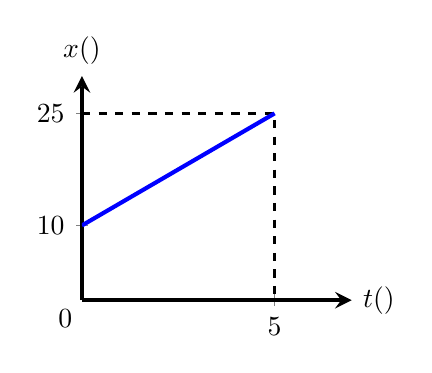
\begin{tikzpicture}  
			\begin{axis}[  ultra thick,
				xmin=0,  
				xmax=7,  
				xtick={0,5},
				ytick={0,10,25},
				ymin=0,  
				ymax=30, 
				samples=300,
				axis lines=center, 
				xlabel=$\xsi{t}{\left(\si{\second}\right)}$, 		ylabel=$\xsi{x}{\left(\si{\meter}\right)}$,
				every axis y label/.style={at=(current axis.above origin),anchor=south},  
				every axis x label/.style={at=(current axis.right of origin),anchor=west},  scale=0.5]
				\draw[line width=1pt, dashed] (axis cs: 0,25)--(axis cs: 5,25)--(axis cs: 5,0);
				\addplot [line width=1.5pt, blue, smooth, domain=0:5] {10+3*x};  
				\coordinate (O) at (axis cs: 0,0);
			\end{axis}  
			\node[below left] at (O) {0};
		\end{tikzpicture}
	}
	\loigiai{}
\end{ex}
% ===================================================================
\begin{ex}
	Một đoàn tàu rời ga chuyển động thẳng nhanh dần, sau 1 phút đạt vận tốc $\SI{40}{\kilo\meter/\hour}$. Gia tốc trung bình của đoàn tàu gần giá trị nào sau đây nhất?	
	\choice
	{$\SI{0.188}{\meter/\second^2}$}
	{$\SI{0.288}{\meter/\second^2}$}
	{$\SI{0.285}{\meter/\second^2}$}
	{\True $\SI{0.185}{\meter/\second^2}$}
	\loigiai{}
\end{ex}
% ===================================================================
\begin{ex}
	Hình vẽ nào sau đây biểu diễn đúng lực tổng hợp $\vec{F}$ của hai lực $\vec{F}_1$ và $\vec{F}_2$?
	\choice
	{\begin{tikzpicture}
			\coordinate (A) at (0,0);
			\coordinate (B) at ($(A)+(2.5,0)$);
			\coordinate (C) at ($(B)+(90:1.5)$);
			\draw[blue, line width=1.5pt, -stealth] (A)--(B);
			\draw[blue, line width=1.5pt, -stealth] (B)--(C);
			\draw[blue, line width=1.5pt, -stealth] (A)--(C);
			\node[below, blue] at ($(A)!0.5!(B)$) {$\vec{F}$};
			\node[right, blue] at ($(B)!0.5!(C)$) {$\vec{F}_2$};
			\node[above left, blue] at ($(A)!0.5!(C)$) {$\vec{F}_1$};
	\end{tikzpicture}}
	{\begin{tikzpicture}
			\coordinate (O) at (0,0);
			\coordinate (A) at (2,0);
			\coordinate (C) at ($(A)+(-60:1.5)$);
			\coordinate (B) at ($(O)+(-60:1.5)$);
			\draw[dashed, line width=1pt] (A)--(C)--(B);
			\draw[-stealth, blue, line width=1.5pt] (O)--(A);
			\draw[-stealth, blue, line width=1.5pt] (O)--(B);
			\draw[-stealth, blue, line width=1.5pt] (O)--(C);
			\node[below left, blue] at ($(O)!0.5!(B)$) {$\vec{F}$};
			\node[above, blue] at ($(O)!0.5!(A)$) {$\vec{F}_1$};
			\node[below, blue] at ($(O)!0.5!(C)$) {$\vec{F}_2$};
	\end{tikzpicture}}
	{\True \begin{tikzpicture}
			\coordinate (O) at (0,0);
			\coordinate (A) at ($(O)+(90:2.5)$);
			\coordinate (B) at ($(O)+(180:2)$);
			\coordinate (C) at ($(A)+(180:2)$);
			\draw[dashed, line width=1pt] (A)--(C)--(B);
			\draw[blue, line width=1.5pt, -stealth] (O)--(A);
			\draw[blue, line width=1.5pt, -stealth] (O)--(C);
			\draw[blue, line width=1.5pt, -stealth] (O)--(B);
			\node[above right, blue] at ($(O)!0.5!(C)$) {$\vec{F}$};
			\node[above, blue] at ($(O)!0.5!(B)$) {$\vec{F}_2$};
			\node[right, blue] at ($(O)!0.5!(A)$) {$\vec{F}_1$};
	\end{tikzpicture}}
	{\begin{tikzpicture}
			\coordinate (O) at (0,0);
			\coordinate (A) at ($(O)+(2,0)$);
			\coordinate (B) at ($(O)+(60:2)$);
			\draw[blue, -stealth, line width=1.5pt] (O)--(A);
			\draw[blue, -stealth, line width=1.5pt] (O)--(B);
			\draw[blue, -stealth, line width=1.5pt] (A)--(B);
			\node[above, blue] at ($(O)!0.5!(A)$) {$\vec{F}_2$};
			\node[right, blue] at ($(A)!0.5!(B)$) {$\vec{F}$};
			\node[left, blue] at ($(O)!0.5!(B)$) {$\vec{F}_1$};
	\end{tikzpicture}}
	\loigiai{}
\end{ex}
% ===================================================================
\begin{ex}
	\immini{Một vật chuyển động thẳng có đồ thị vận tốc - thời gian như hình bên. Tính chất chuyển động của vật là	
		\choice
		{Chuyển động chậm dần đều theo chiều dương rồi nhanh dần đều theo chiều âm}
		{Chuyển động nhanh dần đều theo chiều dương rồi chậm dần đều theo chiều âm}
		{\True Chuyển động nhanh dần đều rồi chậm dần đều theo chiều dương}
		{Chuyển động nhanh dần đều rồi chậm dần đều theo chiều âm}}
	{
		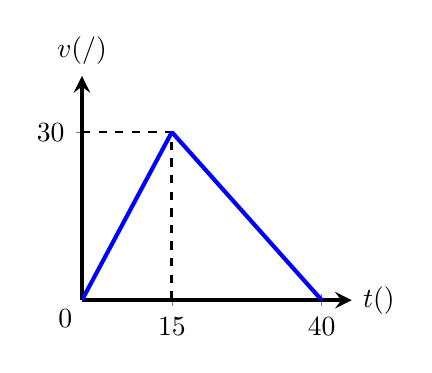
\begin{tikzpicture}  
			\begin{axis}[  ultra thick,
				xmin=0,  
				xmax=45,  
				xtick={0,15,40},
				ytick={0,30},
				ymin=0,  
				ymax=40, 
				samples=300,
				axis lines=center, 
				xlabel=$\xsi{t}{\left(\si{\second}\right)}$, 		ylabel=$\xsi{v}{\left(\si{\meter/\second}\right)}$,
				every axis y label/.style={at=(current axis.above origin),anchor=south},  
				every axis x label/.style={at=(current axis.right of origin),anchor=west},  scale=0.5]
				\draw[line width=1pt, dashed] (axis cs: 0,30)--(axis cs: 15,30)--(axis cs: 15,0);
				\addplot [line width=1.5pt, blue, smooth, domain=0:15] {2*x};  
				\addplot [line width=1.5pt, blue, smooth, domain=15:40] {30-1.2*(x-15)}; 
				\coordinate (O) at (axis cs: 0,0);
			\end{axis}  
			\node[below left] at (O) {0};
		\end{tikzpicture}
	}
	\loigiai{}
\end{ex}
% ===================================================================
\begin{ex}
	Một lực không đổi tác dụng vào một vật có khối lượng $\SI{5.0}{\kilogram}$ làm vận tốc của nó tăng dần từ $\SI{2.0}{\meter}$ đến $\SI{8.0}{\meter/\second}$ trong $\SI{3.0}{\second}$. Độ lớn lực tác dụng vào vật là
	\choice
	{\True $\SI{10}{\newton}$}
	{$\SI{5}{\newton}$}
	{$\SI{15}{\newton}$}
	{$\SI{1}{\newton}$}
	\loigiai{}
\end{ex}
% ===================================================================
\begin{ex}
	Cho biết khối lượng của Trái Đất là $M=\SI{6E24}{\kilogram}$; khối lượng của một hòn đá $m=\SI{2.3}{\kilogram}$; gia tốc trọng trường là $g=\SI{9.81}{\meter/\second^2}$. Hòn đá hút Trái Đất một lực có độ lớn xấp xỉ
	\choice
	{$\SI{15.82}{\newton}$}
	{$\SI{20.24}{\newton}$}
	{\True $\SI{22.56}{\newton}$}
	{$\SI{32}{\newton}$}
	\loigiai{}
\end{ex}
% ===================================================================
\begin{ex}
	Một dòng sông rộng $\SI{100}{\meter}$ và dòng nước chảy với vận tốc $\SI{3}{\meter/\second}$ so với bờ. Một chiếc thuyền đi ngang sông với vận tốc $\SI{4}{\meter/\second}$ so với dòng nước. Quãng đường mà thuyền đi được khi sang đến bờ bên kia là
	\choice
	{$\SI{150}{\meter}$}
	{\True $\SI{125}{\meter}$}
	{$\SI{100}{\meter}$}
	{$\SI{50}{\meter}$}
	\loigiai{}
\end{ex}
% ===================================================================
\begin{ex}
	Một vật có khối lượng $\SI{70}{\kilogram}$ chuyển động thẳng đều trên mặt sàn nằm ngang dưới tác dụng của lực kéo không đổi và có độ lớn $\SI{210}{\newton}$ theo phương ngang. Lấy $g=\SI{10}{\meter/\second^2}$. Hệ số ma sát trượt giữa vật và sàn là
	\choice
	{\True $0,3$}
	{$0,147$}
	{$3,3$}
	{$0,05$}
	\loigiai{}
\end{ex}
% ===================================================================
\begin{ex}
	Một vật khối lượng $\SI{2.5}{\kilogram}$ rơi thẳng đứng từ độ cao $\SI{100}{\meter}$ không vận tốc đầu, sau $\SI{20}{\second}$ thì chạm đất. Lấy gia tốc trọng trường $g=\SI{10}{\meter/\second^2}$. Nếu coi lực cản không khí tác dụng lên vật trong quá trình rơi là không đổi thì độ lớn của lực cản là
	\choice
	{$\SI{20}{\newton}$}
	{$\SI{40}{\newton}$}
	{\True $\SI{23.75}{\newton}$}
	{$\SI{25}{\newton}$}
	\loigiai{}
\end{ex}
% ===================================================================
\begin{ex}
	Một vật chuyển động nhanh dần đều không vận tốc đầu. Trong giây thứ nhất vật đi được đoạn đường $s_1=\SI{3}{\meter}$, trong giây thứ hai vật đi được quãng đường $s_2$ bằng	
	\choice
	{$\SI{6}{\meter}$}
	{$\SI{3}{\meter}$}
	{\True $\SI{9}{\meter}$}
	{$\SI{12}{\meter}$}
	\loigiai{}
\end{ex}
% ===================================================================
\begin{ex}
	Một quả bóng có khối lượng $\SI{300}{\gram}$ bay với vận tốc $\SI{72}{\kilo\meter/\hour}$ đến đập vuông góc vào một bức tường thẳng đứng rồi bật trở lại theo phương cũ với vận tốc $\SI{54}{\kilo\meter/\hour}$. Thời gian va chạm $\SI{0.14}{\second}$. Lực do tường tác dụng lên quả bóng có độ lớn là
	\choice
	{\True $\SI{75}{\newton}$}
	{$\SI{70}{\newton}$}
	{$\SI{85}{\newton}$}
	{$\SI{65}{\newton}$}
	\loigiai{}
\end{ex}
\Closesolutionfile{ans}
\section{Câu trắc nghiệm đúng/sai} 
\textit{Thí sinh trả lời từ câu 1 đến câu 4. Trong mỗi ý \textbf{a)}, \textbf{b)}, \textbf{c)}, \textbf{d)} ở mỗi câu, thí sinh chọn đúng hoặc sai}
\setcounter{ex}{0}\\
\Opensolutionfile{ans}[ans/G10-FINAL-SEM1-001-TF]
% ===================================================================
\begin{ex}
	Nhận định các phát biểu sau về vai trò của lực ma sát nghỉ.\\
	Lực ma sát nghỉ
	\choiceTF[t]
	{\True đóng vai trò là lực phát động trong trường hợp chuyển động của người đi bộ, xe đạp, ô tô, tàu hỏa, \dots}
	{\True giúp ta cầm, nắm các vật}
	{giúp xe chuyển động chậm lại khi hãm phanh}
	{\True đóng vai trò truyền chuyển động bằng dây curoa trong các máy móc, băng chuyền, \dots}
	\loigiai{}
\end{ex}
% ===================================================================
\begin{ex}
	\immini{Một quả khúc côn cầu có khối lượng $\SI{0.30}{\kilogram}$ đang nằm trên mặt băng cứng, hoàn toàn nhẵn nằm ngang, thì chịu tác dụng đồng thời của hai cú đánh như hình bên. Lực $\vec{F}_1$ do cú đánh thứ nhất có độ lớn $\SI{5.0}{\newton}$ làm với trục $x$ về phía dưới một góc $\SI{20}{\degree}$. Lực $\vec{F}_2$ do cú đánh thứ hai có độ lớn $\SI{8.0}{\newton}$ làm với trục $x$ về phía trên một góc $\SI{60}{\degree}$.} {\includegraphics[scale=0.35]{../figs/D10-CK1-002-2}}
	\choiceTF[t]
	{\True Hợp lực tác dụng lên quả khúc côn cầu có độ lớn $\SI{10.14}{\newton}$}
	{\True Sau cú đánh, quả khúc côn cầu chuyển động theo hướng hợp với trục $x$ góc $\SI{31}{\degree}$}
	{\True Trọng lực tác dụng lên quả khúc côn cầu không gây ra gia tốc cho nó}
	{\True Gia tốc của quả khúc côn cầu ngay sau cú đánh kép xấp xỉ $\SI{34}{\meter/\second^2}$}
	\loigiai{}
\end{ex}

% ===================================================================
\begin{ex}
	\immini{	Huyền thoại điền kinh Usain Bolt người Jamaica đã lập kỉ lục thế giới ở nội dung chạy $\SI{100}{\meter}$ vào tháng 8/2009 tại Berlin. Usain Bolt đã hoàn thành cự li trên với thời gian $\SI{9.58}{\second}$. Ta giả sử rằng Bolt tăng tốc đều trong $\SI{3.00}{\second}$ đầu tiên để đạt tốc độ tối đa và duy trì tốc độ đó trong suốt phần còn lại của cuộc đua.}
	{\includegraphics[scale=0.08]{../figs/D10-CK1-001-5}}
	\choiceTF[t]
	{Chuyển động của Usain Bolt là chuyển động thẳng nhanh dần đều}
	{\True Tốc độ của Usain Bolt khi về đến đích xấp xỉ $\SI{12.38}{\meter/\second}$}
	{Gia tốc trong giai đoạn tăng tốc của Usain Bolt là khoảng $\SI{6}{\meter/\second^2}$}
	{\True Usain Bolt đã duy trì tốc độ tối đa của mình trên đoạn đường dài $\SI{81.46}{\meter}$}
	\loigiai{}
\end{ex}
% ===================================================================
\begin{ex}
	\immini{Một vật nhỏ có khối lượng $\SI{5.0}{\kilogram}$ được kéo bằng sợi dây trên sàn nằm ngang. Sợi dây nhẹ, không dãn và làm góc $\SI{25}{\degree}$ so với phương ngang. Hệ số ma sát trượt giữa vật và mặt sàn là $0,15$. Lực kéo tác dụng lên dây có độ lớn $F=\SI{12}{\newton}$. Lấy $g=\SI{9.8}{\meter/\second^2}$.}
	{\begin{tikzpicture}
			\coordinate (O) at (0,0);
			\coordinate (A) at ($(O)+(2.5,0)$);
			\coordinate (B) at ($(O)+(25:2)$);
			\filldraw[color=orange!80!brown] (-0.5,-0.25) rectangle (0.5,0.25);
			\draw[line width=6pt, color=gray] (-2.5,-0.36)--(2.5,-0.36);
			\draw[-stealth, blue, line width=1.5pt] (O)--(B);
			\draw[dashed, line width=1pt] (O)--(A);
			\tkzMarkAngle[size=0.75cm,color=red, line width=1.2pt](A,O,B);
			\tkzLabelAngle[color=black,pos=1.2](A,O,B){$\SI{25}{\degree}$};
			\node[above, blue]at(B) {$\vec{F}$};
	\end{tikzpicture}}
	\choiceTF[t]
	{Phản lực của mặt sàn tác dụng lên vật bằng $\SI{49}{\newton}$}
	{\True Lực ma sát trượt tác dụng lên vật có độ lớn xấp xỉ $\SI{6.6}{\newton}$}
	{Gia tốc của vật xấp xỉ $\SI{1.08}{\meter/\second^2}$}
	{Người ta tăng dần lực kéo $F$, ngay khi lực kéo có độ lớn $\SI{49}{\newton}$ thì vật bị nâng khỏi mặt sàn}
	\loigiai{}
\end{ex}
\Closesolutionfile{ans}
\section{Câu trắc nghiệm trả lời ngắn} \textit{Thí sinh trả lời từ câu 1 đến câu 6}
\setcounter{ex}{0}
\Opensolutionfile{ans}[ans/G10-FINAL-SEM1-001-TL]
% ===============================================================
\begin{ex}
	Một chất điểm chuyển động thẳng có phương trình vận tốc theo thời gian dạng $v=15-3t$, trong đó $t$ tính bằng giây và $v$ tính bằng $\si{\meter/\second}$. Tính tốc độ trung bình của chất điểm trong khoảng thời gian từ $t_1=\SI{0}{\second}$ đến $t_2=\SI{2}{\second}$ theo đơn vị mét/giây $\left(\si{\meter/\second}\right)$.
	\shortans[oly]{12}
	\loigiai{
		
	}
\end{ex}
% ===============================================================
\begin{ex}
	Một vật khối lượng $m=\SI{1.5}{\kilogram}$ bắt đầu chuyển động nhanh dần đều trên mặt phẳng ngang dưới tác dụng của lực kéo theo phương ngang, độ lớn $F_{\mathrm{k}}=\SI{7.5}{\newton}$. Hệ số ma sát giữa vật và mặt phẳng ngang là $\mu=0,2$. Lấy $g=\SI{10}{\meter/\second^2}$. Tính gia tốc của vật theo đơn vị $\si{\meter/\second^2}$.
	\shortans[oly]{3}
	\loigiai{
		
	}
\end{ex}
% ===============================================================
\begin{ex}
	\immini{Một vòng đệm bằng đồng có đường kính ngoài và đường kính trong lần lượt là $\SI{4.50}{\centi\meter}$ và $\SI{1.25}{\centi\meter}$. Bề dày của vòng đệm là $\SI{1.50}{\milli\meter}$. Đồng có khối lượng riêng là $\SI{8600}{\kilogram/\meter^3}$. Lấy gia tốc trọng trường $g=\SI{9.8}{\meter/\second^2}$, $\pi=3,14$. Trọng lượng của vòng đệm trên là bao nhiêu newton $\left(\si{\newton}\right)$? \textit{(Kết quả làm tròn đến chữ số hàng phần mười)}.}
	{
		\includegraphics[scale=0.4]{../figs/D10-CK1-001-3}
	}
	\shortans[oly]{0,2}
	\loigiai{
		
	}
\end{ex}

% ===============================================================
\begin{ex}
	\immini{Một khối hộp có dạng hình lập phương nặng $\SI{1}{\kilogram}$  đặt trong nước nguyên chất có khối lượng riêng $\rho=\SI{1000}{\kilogram/\meter^3}$. Mỗi cạnh của khối hộp có độ dài $\SI{10}{\centi\meter}$. Cho $g=\SI{10}{\meter/\second^2}$. Tính lực đẩy Archimedes tác dụng lên khối hộp nếu nó được nhúng hoàn toàn trong nước. \textit{(Kết quả tính theo đơn vị newton $\left(\si{\newton}\right)$)}.}
	{\includegraphics[scale=0.4]{../figs/D10-CK1-001-1}}
	\shortans[oly]{10}
	\loigiai{
		
	}
\end{ex}
% ===============================================================
\begin{ex}
	\immini{Một cơ hệ bố trí như hình bên được sử dụng trong bệnh viện để hỗ trợ tác dụng lực kéo ngang lên chân bị thương của bệnh nhân. Lấy gia tốc trọng trường $g=\SI{9.8}{\meter/\second^2}$. Tính độ lớn hợp lực kéo ngang tác dụng lên giá đỡ bàn chân theo đơn vị newton $\left(\si{\newton}\right)$. \textit{(Kết quả làm tròn đến chữ số hàng đơn vị)}.}{
		\includegraphics[scale=0.35]{../figs/D10-CK1-001-6}
	}
	\shortans[oly]{105}
	\loigiai{
		
	}
\end{ex}
% ===============================================================
\begin{ex}
	\immini{Một vật khối lượng $m=\SI{1}{\kilogram}$ có thể trượt trên mặt phẳng nghiêng góc $\alpha=\SI{30}{\degree}$ so với mặt ngang. Hệ số ma sát giữa vật và mặt phẳng nghiêng là $\mu=0,2$. Lực $\vec{F}$  không đổi tác dụng vào vật có phương nằm ngang (hình vẽ). Lấy $g=\SI{10}{\meter/\second^2}$.	Xác định độ lớn của lực $\vec{F}$ để vật trượt đều lên mặt phẳng nghiêng. \textit{(Kết quả tính theo đơn vị $\si{\newton}$ và làm tròn đến chữ số hàng phần mười)}.
	}
	{\includegraphics[scale=0.8]{../figs/D10-CK1-001-2}}
	\shortans[oly]{ 8,8}
	\loigiai{
		
	}
\end{ex}
\Closesolutionfile{ans}
\begin{center}
	\textbf{--- HẾT ---}
\end{center}
%\chapter{ĐỀ 02}
%\begin{center}
	\begin{tabular}{M{9.25cm}M{8.75cm}}
		\textbf{TRUNG TÂM MANABIE}& \textbf{ÔN TẬP KIỂM TRA CUỐI HỌC KÌ I}\\
		\textbf{MÃ ĐỀ: 002}& \textbf{Bài thi môn: VẬT LÝ 10}\\
		\textit{(Đề thi có 04 trang)}& \textit{Thời gian làm bài: 45 phút, không kể phát đề}
		
		\noindent\rule{4cm}{0.8pt} \\
	\end{tabular}
\end{center}
\setcounter{section}{0}
\begin{center}
	\textbf{\large BẢNG ĐÁP ÁN}
\end{center}
\section{}
\inputansbox{10}{ans/G10-FINAL-SEM1-002-TN}
\section{}
\inputansbox[2]{2}{ans/G10-FINAL-SEM1-002-TF}
\section{}
\inputansbox[3]{6}{ans/G10-FINAL-SEM1-002-TL}\newpage
%\begin{center}
	\begin{tabular}{M{9.25cm}M{8.75cm}}
		\textbf{TRUNG TÂM MANABIE}& \textbf{ÔN TẬP KIỂM TRA CUỐI HỌC KÌ I}\\
		\textbf{MÃ ĐỀ: 002}& \textbf{Bài thi môn: VẬT LÝ 10}\\
		\textit{(Đề thi có 04 trang)}& \textit{Thời gian làm bài: 50 phút, không kể phát đề}
		\noindent\rule{4cm}{0.8pt} \\
	\end{tabular}
\end{center}
\setcounter{section}{0}
\vspace{-1cm}
\section{Câu trắc nghiệm nhiều phương án lựa chọn}
\textit{Thí sinh trả lời từ câu 1 đến câu 18. Mỗi câu hỏi thí sinh chọn một phương án}
\setcounter{ex}{0}
\Opensolutionfile{ans}[ans/G10-FINAL-SEM1-002-TN]
% ===================================================================
\begin{ex}
	Người ta thường dùng quãng đường đi được trong cùng một đơn vị thời gian để xác định độ nhanh, chậm của chuyển động. Đại lượng này gọi là
	\choice
	{vận tốc trung bình}
	{\True tốc độ trung bình}
	{tốc độ tức thời}
	{vận tốc tức thời}
	\loigiai{}
\end{ex}
% ===================================================================
\begin{ex}
	Điều nào sau đây là \textbf{sai} khi nói về trọng lực?
	\choice
	{Trọng lực được xác định bởi biểu thức $\vec{P}=m\cdot\vec{g}$}
	{Điểm đặt của trọng lực là trọng tâm của vật}
	{\True Trọng lực có độ lớn tỉ lệ nghịch với khối lượng của vật}
	{Trọng lực là lực hút của Trái Đất tác dụng lên vật}
	\loigiai{}
\end{ex}
% ===================================================================
\begin{ex}
	Trong một cơn giông, một cành cây bị gãy và bay trúng vào một cửa kính, làm vỡ kính. Chọn nhận xét đúng.	
	\choice
	{Lực của cành cây tác dụng lên tấm kính lớn hơn lực của tấm kính tác dụng vào cành cây}
	{\True Lực của cành cây tác dụng lên tấm kính có độ lớn bằng lực của tấm kính tác dụng vào cành cây}
	{Lực của cành cây tác dụng lên tấm kính nhỏ hơn lực của tấm kính tác dụng vào cành cây}
	{Cành cây không tương tác với tấm kính khi làm vỡ kính}
	\loigiai{}
\end{ex}
% ===================================================================
\begin{ex}
	Chỉ ra phát biểu \textbf{sai}.\\
	Độ lớn của lực ma sát trượt	
	\choice
	{\True phụ thuộc vào diện tích tiếp xúc của vật}
	{không phụ thuộc vào tốc độ của vật}
	{tỉ lệ với độ lớn của áp lực}
	{phụ thuộc vào vật liệu và tính chất của hai mặt tiếp xúc}
	\loigiai{}
\end{ex}
% ===================================================================
\begin{ex}
	Lực đẩy Archimedes phụ thuộc vào các yếu tố:
	\choice
	{trọng lượng riêng của chất lỏng và thể tích của vật}
	{trọng lượng của chất lỏng và thể tích của phần chất lỏng bị vật chiếm chỗ}
	{\True trọng lượng riêng của chất lỏng và thể tích của phần chất lỏng bị vật chiếm chỗ}
	{trọng lượng riêng của vật và thể tích của phần chất lỏng bị vật chiếm chỗ}
	\loigiai{}
\end{ex}
% ===================================================================
\begin{ex}
	Một người kéo xe hàng trên mặt sàn nằm ngang, lực tác dụng lên người để làm người chuyển động về phía trước là lực mà
	\choice
	{người tác dụng vào xe}
	{xe tác dụng vào người}
	{người tác dụng vào mặt đất}
	{\True mặt đất tác dụng vào người}
	\loigiai{}
\end{ex}
% ===================================================================
\begin{ex}
	Khi vật đang chuyển động thẳng và đổi chiều chuyển động thì đại lượng nào sau đây đổi dấu?	
	\choice
	{Tốc độ trung bình và vận tốc trung bình}
	{Tốc độ tức thời}
	{\True Độ dịch chuyển và vận tốc}
	{Quãng đường và độ dịch chuyển}
	\loigiai{}
\end{ex}
% ===================================================================
\begin{ex}
	Câu nào sau đây là \textbf{sai} khi nói về lực căng dây?
	\choice
	{Lực căng dây có bản chất là lực đàn hồi}
	{Lực căng dây có điểm đặt là điểm mà đầu dây tiếp xúc với vật}
	{Lực căng có phương trùng với chính sợi dây, chiều hướng từ hai đầu vào phần giữa của sợi dây}
	{\True Lực căng có thể là lực kéo hoặc lực nén}
	\loigiai{}
\end{ex}
% ===================================================================
\begin{ex}
	Các giọt mưa rơi thẳng đứng với tốc độ $\SI{6}{\kilo\meter/\hour}$. Một người đi bộ trên đường thẳng nằm ngang với tốc độ $\SI{8}{\kilo\meter/\hour}$. Vận tốc tương đổi của giọt mưa đối với người có độ lớn là
	\choice
	{$\SI{7}{\kilo\meter/\hour}$}
	{\True $\SI{10}{\kilo\meter/\hour}$}
	{$\SI{14}{\kilo\meter/\hour}$}
	{$\SI{2}{\kilo\meter/\hour}$}
	\loigiai{}
\end{ex}
% ===================================================================
\begin{ex}
	Một xe có khối lượng $m=\SI{5}{\text{tấn}}$ đang đứng yên trên mặt phẳng nghiêng $\SI{30}{\degree}$ so với phương ngang. Độ lớn của lực ma sát tác dụng lên xe
	\choice
	{lớn hơn trọng lượng của xe}
	{bằng trọng lượng của xe}
	{bằng độ lớn của thành phần trọng lực vuông góc với mặt phẳng nghiêng}
	{\True bằng độ lớn của thành phần trọng lực song song với mặt phẳng nghiêng}
	\loigiai{}
\end{ex}
% ===================================================================
\begin{ex}
	Một thỏi nhôm và một thỏi thép có thể tích bằng nhau cùng được nhúng chìm trong nước. Nhận xét nào sau đây là \textbf{đúng}?	
	\choice
	{Thỏi nào chìm sâu hơn thì lực đẩy Archimedes tác dụng lên thỏi đó lớn hơn}
	{\True Hai thỏi nhôm và thép đều chịu tác dụng của lực đẩy Archimedes như nhau vì chúng chiếm thể tích trong nước như nhau}
	{Hai thỏi nhôm và thép đều chịu tác dụng của lực đẩy Archimedes như nhau vì chúng cùng được nhúng trong nước}
	{Thép có trọng lượng riêng lớn hơn nhôm nên thỏi thép chịu tác dụng của lực đẩy Archimedes lớn hơn}
	\loigiai{}
\end{ex}

% ===================================================================
\begin{ex}
	Lực hãm không đổi có độ lớn $F$ tác dụng vào vật khối lượng $m$ đang chuyển động với vận tốc ban đầu $v$. Sau thời gian $t$ bao lâu thì vật đó đứng yên?
	\choice
	{$t=\dfrac{vF}{m}$}
	{\True $t=\dfrac{mv}{F}$}
	{$t=\dfrac{F}{mv}$}
	{$t=\dfrac{v}{mF}$}
	\loigiai{}
\end{ex}
% ===================================================================
\begin{ex}
	Một xe ô tô đang chạy trên đường thẳng nằm ngang với tốc độ $v_0=\SI{72}{\kilo\meter/\hour}$ thì tắt máy. Quãng đường ô tô đi được từ lúc tắt máy đến khi dừng hẳn là $\SI{40}{\meter}$. Lấy gia tốc trọng trường $g=\SI{10}{\meter/\second^2}$. Hệ số ma sát giữa bánh xe và mặt đường là
	\choice
	{\True $\mu=0,5$}
	{$\mu=0,4$}
	{$\mu=0,3$}
	{$\mu=0,6$}
	\loigiai{}
\end{ex}
% ===================================================================
\begin{ex}
	Một vật có khối lượng $\SI{3}{\kilogram}$ đang chuyển động thẳng đều với vận tốc $v_0=\SI{2}{\meter/\second}$ thì chịu tác dụng của một lực $\SI{9}{\newton}$ cùng chiều với $\vec{v}_0$. Vật sẽ chuyển động $\SI{10}{\meter}$ tiếp theo trong thời gian	
	\choice
	{\True $\SI{2}{\second}$}
	{$\SI{3}{\second}$}
	{$\SI{4}{\second}$}
	{$\SI{5}{\second}$}
	\loigiai{}
\end{ex}
% ===================================================================
\begin{ex}
	Thể tích của một miếng sắt là $\SI{2}{\deci\meter^3}$. Cho khối lượng riêng của nước là $\SI{1000}{\kilogram/\meter^3}$. Lấy $g=\SI{9.8}{\meter/\second^2}$. Lực đẩy tác dụng lên miếng sắt khi nhúng chìm trong nước có giá trị là
	\choice
	{$\SI{25}{\newton}$}
	{$\SI{20}{\newton}$}
	{\True $\SI{19.6}{\newton}$}
	{$\SI{19600}{\newton}$}
	\loigiai{}
\end{ex}
% ===================================================================
\begin{ex}
	\immini{Một chất điểm chịu tác dụng của ba lực $\vec{F}_1$, $\vec{F}_2$, $\vec{F}_3$ có cùng độ lớn $\SI{12}{\newton}$. Biết góc tạo bởi các lực $\left(\vec{F}_1, \vec{F}_2\right)=\left(\vec{F}_2,\vec{F}_3\right)=\SI{60}{\degree}$. Hợp lực của ba lực này có độ lớn 	
		\choice
		{$\SI{6}{\newton}$}
		{\True $\SI{24}{\newton}$}
		{$\SI{10.4}{\newton}$}
		{$\SI{20.8}{\newton}$}}
	{\vspace{-0.5cm}\begin{tikzpicture}
			\coordinate (O) at (0,0);
			\coordinate (F1) at ($(O)+(30:2)$);
			\coordinate (F2) at ($(O)+(90:2)$);
			\coordinate (F3) at ($(O)+(150:2)$);
			\tkzMarkAngle[size=0.6cm,color=red, line width=1.2pt](F1,O,F2);
			\tkzLabelAngle[color=black,pos=1.0](F1,O,F2){$\SI{60}{\degree}$};
			\tkzMarkAngle[size=0.75cm,color=red, line width=1.2pt](F2,O,F3);
			\tkzLabelAngle[color=black,pos=1.2](F2,O,F3){$\SI{60}{\degree}$};
			\draw[-stealth, line width=1.5pt, blue] (O)--(F1);
			\draw[-stealth, line width=1.5pt, blue] (O)--(F2);
			\draw[-stealth, line width=1.5pt, blue] (O)--(F3);
			\node[above, blue] at (F1) {$\vec{F}_1$};
			\node[above, blue] at (F2) {$\vec{F}_2$};
			\node[above, blue] at (F3) {$\vec{F}_3$};
	\end{tikzpicture}}
	
	\loigiai{}
\end{ex}
% ===================================================================
\begin{ex}
	Vật nhỏ khối lượng $m=\SI{5}{\kilogram}$ nằm yên trên mặt phẳng ngang. Tác dụng lên vật lực kéo $F=\SI{12}{\newton}$ theo phương ngang. Lấy $g=\SI{10}{\meter/\second^2}$. Hệ số ma sát giữa vật và mặt phẳng ngang là $0,2$.	  Sau khi vật trượt được $\SI{5}{\meter}$ thì ngừng tác dụng lực. Quãng đường dài nhất vật đi từ lúc bắt đầu chuyển động là
	\choice
	{$\SI{8}{\meter}$}
	{\True $\SI{6}{\meter}$}
	{$\SI{1}{\meter}$}
	{$\SI{10}{\meter}$}
	\loigiai{}
\end{ex}
% ===================================================================
\begin{ex}
	Một sợi dây có thể treo một vật đứng yên có khối lượng tối đa là $\SI{50}{\kilogram}$ mà không bị đứt. Dùng sợi dây này để kéo một vật khác có khối lượng $\SI{45}{\kilogram}$ lên cao theo phương thẳng đứng. Lấy gia tốc trọng trường $g=\SI{10}{\meter/\second^2}$. Gia tốc lớn nhất mà vật có thể có để dây không bị đứt là
	\choice
	{\True $\SI{1.1}{\meter/\second^2}$}
	{$\SI{11.1}{\meter/\second^2}$}
	{$\SI{21.1}{\meter/\second^2}$}
	{$\SI{10.5}{\meter/\second^2}$}
	\loigiai{}
\end{ex}
\Closesolutionfile{ans}
\section{Câu trắc nghiệm đúng/sai} 
\textit{Thí sinh trả lời từ câu 1 đến câu 4. Trong mỗi ý \textbf{a)}, \textbf{b)}, \textbf{c)}, \textbf{d)} ở mỗi câu, thí sinh chọn đúng hoặc sai}
\setcounter{ex}{0}\\
\Opensolutionfile{ans}[ans/G10-FINAL-SEM1-002-TF]
% ===================================================================
\begin{ex}
	Một quyển sách đang được đặt nằm yên trên mặt bàn nằm ngang.	Nhận định các phát biểu sau đây:
	\choiceTF[t]
	{\True Trọng lực tác dụng lên quyển sách cũng là lực hấp dẫn do Trái Đất tác dụng lên sách}
	{Trọng lực của quyển sách và phản lực của mặt bàn tác dụng lên sách có cùng bản chất}
	{Quyển sách chịu tác dụng của lực ma sát nghỉ có phương song song với mặt bàn}
	{Trọng lực tác dụng lên sách luôn có độ lớn bằng phản lực của bàn tác dụng lên sách}
	\loigiai{}
\end{ex}

% ===================================================================
\begin{ex}
	Hai xe đồ chơi A và B chuyển động trên mặt phẳng nằm ngang với tốc độ lần lượt là $\SI{50}{\centi\meter/\second}$ và $\SI{150}{\centi\meter/\second}$. Xe B tới va chạm với xe A từ phía sau. Sau va chạm, hai xe chuyển động với cùng tốc độ $\SI{100}{\centi\meter/\second}$. Biết rằng trong suốt quá trình va chạm, các vector vận tốc không đổi hướng.
	\choiceTF[t]
	{Độ lớn lực do xe A tác dụng lên xe B lớn hơn độ lớn lực do xe B tác dụng lên xe A}
	{Xe A tác dụng lực lên xe B trước, sau đó xe B mới tác dụng lực lên xe A}
	{Gia tốc của hai xe trong quá trình va chạm là bằng nhau}
	{Khối lượng xe A lớn hơn khối lượng xe B}
	\loigiai{}
\end{ex}
% ===================================================================
\begin{ex}
	Một quả cầu đặc được làm bằng nhôm. Người ta treo quả cầu bên dưới một lực kế trong không khí, lực kế chỉ $\SI{7.1}{\newton}$. Biết khối lượng riêng của nhôm, nước và dầu lần lượt là $\rho_1=\SI{2700}{\kilogram/\meter^3}$, $\rho_2=\SI{1000}{\kilogram/\meter^3}$, $\SI{800}{\kilogram/\meter^3}$. Lấy gia tốc trọng trường $g=\SI{9.8}{\meter/\second^2}$. Thể tích khối cầu bán kính $r$ được xác định bởi $V=\dfrac{4}{3}\pi r^3$.
	\choiceTF[t]
	{\True Bán kính quả cầu nhôm là $\SI{4}{\centi\meter}$}
	{\True Nhúng quả cầu chìm trong dầu thì số chỉ lực kế là $\SI{5}{\newton}$}
	{Nếu nhúng quả cầu vào trong nước, quả cầu chỉ chìm một phần}
	{\True Để quả cầu lơ lửng trong dầu, người ta phải khoét rỗng phần bên trong của quả cầu với bán kính phần rỗng là $\SI{35.6}{\milli\meter}$}
	\loigiai{}
\end{ex}
% ===================================================================
\begin{ex}
	\immini{Một vật nhỏ có khối lượng $\SI{15}{\kilogram}$ được giữ nằm yên trên mặt phẳng nghiêng không ma sát với góc nghiêng $\SI{27}{\degree}$ so với mặt ngang bằng một sợi dây nhẹ, không dãn như hình. Lấy $g=\SI{9.8}{\meter/\second^2}$. }{\vspace{-0.5cm}\includegraphics[scale=0.25]{../figs//D10-CK1-002-1}}
	\choiceTF[t]
	{Phản lực của mặt phẳng nghiêng tác dụng lên vật cân bằng với trọng lực của vật}
	{\True Lực căng của sợi dây là $\SI{67}{\newton}$}
	{\True Khi cắt đứt dây giữ vật thì vật sẽ trượt xuống với gia tốc có độ lớn $\SI{4.4}{\meter/\second^2}$}
	{Nếu tăng góc nghiêng thì áp lực của vật lên mặt phẳng nghiêng tăng lên}
	\loigiai{2,6}
\end{ex}
\Closesolutionfile{ans}
\section{Câu trắc nghiệm trả lời ngắn} \textit{Thí sinh trả lời từ câu 1 đến câu 6}
\setcounter{ex}{0}
\Opensolutionfile{ans}[ans/G10-FINAL-SEM1-002-TL]
% ===============================================================
\begin{ex}
	Một ô tô đang chạy với tốc độ $\SI{10}{\meter/\second}$ trên một đoạn đường thẳng thì người lái xe tăng ga cho ô tô chạy nhanh dần đều. Sau $\SI{20}{\second}$, ô tô đạt tốc độ $\SI{14}{\meter/\second}$. Tính quãng đường ô tô đi được sau $\SI{50}{\second}$ kể từ khi tăng ga theo đơn vị mét $\left(\si{\meter}\right)$.	
	\shortans[oly]{750}
	\loigiai{
		
	}
\end{ex}
% ===============================================================
\begin{ex}
	\immini{Một đèn tín hiệu giao thông có trọng lượng $\SI{1.00E2}{\newton}$ được treo cố định nhờ ba sợi dây như hình bên. Hai sợi dây cáp ở trên hợp với phương ngang các góc lần lượt $\SI{37.0}{\degree}$ và $\SI{53.0}{\degree}$. Xác định độ lớn lực căng trên dây cáp $T_2$ theo đơn vị newton $\left(\si{\newton}\right)$. \textit{(Kết quả làm tròn đến chữ số hàng phần mười)}.}	
	{\vspace{-0.5cm}
		\includegraphics[scale=0.3]{../figs//D10-CK1-002-4}}
	\shortans[oly]{79,9}
	\loigiai{
		
	}
\end{ex}
% ===============================================================
\begin{ex}
	\immini{Một người đẩy máy cắt cỏ có khối lượng $\SI{15}{\kilogram}$ di chuyển với một lực có độ lớn xem như không đổi bằng $\SI{80}{\newton}$ theo phương của giá đẩy như hình bên. Biết góc tạo bởi giá đẩy và phương ngang là $\SI{45}{\degree}$. Nếu từ trạng thái nghỉ, người này tác dụng lực để tăng tốc cho máy đạt tốc độ $\SI{1.2}{\meter/\second}$ trong $\SI{3}{\second}$ thì độ lớn lực ma sát trong giai đoạn này là bao nhiêu newton ($\si{\newton}$)? \textit{(Kết quả làm tròn đến chữ số hàng phần mười).}}
	{\vspace{-0.5cm}
		\includegraphics[scale=0.3]{../figs/D10-CK1-002-3}}
	\shortans[oly]{50,6}
	\loigiai{
		
	}
\end{ex}
% ===============================================================
\begin{ex}
	\immini{Thùng hàng có trọng lượng $\SI{1000}{\newton}$ đang nằm yên trên mặt sàn nằm ngang thì chịu tác dụng bởi lực $\vec{F}$ có hướng như hình bên. Độ lớn lực $\vec{F}$ là $\SI{300}{\newton}$. Xác định tỉ số áp lực của thùng hàng lên mặt sàn trong trường hợp a và trường hợp b.	\textit{(Kết quả làm tròn đến chữ số hàng phần mười)}.}
	{\vspace{-0.5cm}\includegraphics[scale=0.4]{../figs/D10-CK1-001-4}}
	\shortans[oly]{1,2}
	\loigiai{
		
	}
\end{ex}
% ===============================================================
\begin{ex}
	\immini{Một vật nhỏ khối lượng $m=\SI{2}{\kilogram}$ đang nằm yên trên mặt bàn nằm ngang thì chịu tác dụng của lực $\vec{F}$ không đổi, theo phương song song với mặt bàn trong khoảng thời gian $\SI{8}{\second}$. Hình bên là đồ thị vận tốc thời gian của vật kể từ khi chịu tác dụng của lực $\vec{F}$. Xem như lực ma sát giữa vật và mặt bàn là không đổi trong suốt quá trình vật chuyển động. Xác định độ lớn của lực $\vec{F}$ theo đơn vị newton $\left(\si{\newton}\right)$. \textit{(Kết quả làm tròn đến chữ số hàng phần mười)}.}
	{\vspace{-0.5cm}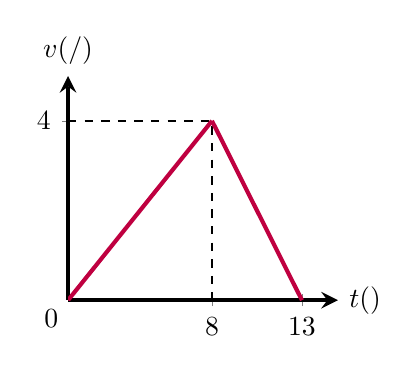
\begin{tikzpicture}  
			\begin{axis}[  ultra thick,scale=0.5,
				xmin=0,  
				xmax=15,  
				xtick={0,8,13},
				ytick={0,4},
				ymin=0,  
				ymax=5, 
				samples=300,
				axis lines=center, 
				xlabel=$\xsi{t}{\left(\si{\second}\right)}$, 		ylabel=$\xsi{v}{\left(\si{\meter/\second}\right)}$,
				every axis y label/.style={at=(current axis.above origin),anchor=south},  
				every axis x label/.style={at=(current axis.right of origin),anchor=west},  ]
				\draw[dashed, line width=0.75pt] (axis cs: 0,4)--(axis cs: 8,4)--(axis cs: 8,0);
				\addplot [line width=1.5pt, purple, smooth, domain=0:8] {0.5*x}; 
				\addplot [line width=1.5pt, purple, smooth, domain=8:13] {4-0.8*(x-8)};   
				\coordinate (O) at (axis cs: 0,0);
			\end{axis}  
			\node[below left] at (O) {0};
	\end{tikzpicture}}
	\shortans[oly]{2,6}
	\loigiai{
		
	}
\end{ex}
% ===============================================================
\begin{ex}
	Lực phát động lớn nhất của một mẫu ô tô đạt được trong điều kiện thử nghiệm là $F=\SI{500}{\newton}$. Cho rằng lực cản không khí $F_c$ tác dụng lên ô tô phụ thuộc vào tốc độ của nó theo biểu thức $F_c=0,2v^2$, trong đó $v$ là tốc độ tính bằng $\si{\meter/\second}$. Xác định tốc độ khi ổn định của ô tô này trong điều kiện thử nghiệm.	
	\shortans[oly]{50}
	\loigiai{
		
	}
\end{ex}
\Closesolutionfile{ans}
\begin{center}
	\textbf{--- HẾT ---}
\end{center}
%\part{ĐỀ KIỂM TRA CUỐI HỌC KÌ I LỚP 11}		
%\chapter{ĐỀ 01}
%\input{../data/G11-FINAL-SEM1-001-DA}\newpage
%\begin{center}
	\begin{tabular}{M{9.25cm}M{8.75cm}}
		\textbf{TRUNG TÂM MANABIE}& \textbf{ÔN TẬP KIỂM TRA CUỐI HỌC KÌ I}\\
		\textbf{MÃ ĐỀ: 001}& \textbf{Bài thi môn: VẬT LÝ 11}\\
		\textit{(Đề thi có 04 trang)}& \textit{Thời gian làm bài: 50 phút, không kể phát đề}
		
		\noindent\rule{4cm}{0.8pt} \\
	\end{tabular}
\end{center}
\setcounter{section}{0}
\section{Câu trắc nghiệm nhiều phương án lựa chọn}
\textit{Thí sinh trả lời từ câu 1 đến câu 18. Mỗi câu hỏi thí sinh chọn một phương án}
\setcounter{ex}{0}
\Opensolutionfile{ans}[ans/G11-FINAL-SEM1-001-TN]
%===================================================================
\begin{ex}
	Tìm phát biểu \textbf{sai} về các điều kiện cần để xảy ra hiện tượng giao thoa sóng cơ. 
	\choice
	{\True hai sóng có cùng biên độ}
	{hai sóng có cùng tần số}
	{hai sóng có cùng phương dao động}
	{hai sóng có độ lệch pha không đổi theo thời gian}
	\loigiai{}
\end{ex}
% ===================================================================
\begin{ex}
	Trên một sợi dây đàn hồi AB đang có sóng dừng với bước sóng $\lambda$. Gọi $d$ là khoảng cách từ một bụng sóng đến một nút sóng. Hệ thức nào sau đây là đúng? 
	\choice
	{$d=\left(\dfrac{k}{2}+\dfrac{1}{2}\right)\lambda$ với $k=0; 1; 2; \dots$}
	{$d=\left(k+\dfrac{1}{4}\right)\lambda$ với $k=0; 1; 2; \dots$}
	{\True $d=\left(\dfrac{k}{2}+\dfrac{1}{4}\right)\lambda$ với $k=0; 1; 2; \dots$}
	{$d=\left(k+\dfrac{1}{2}\right)\lambda$ với $k=0; 1; 2; \dots$}
	\loigiai{$d=\left(2k+1\right)\dfrac{\lambda}{4}\Rightarrow d=\left(\dfrac{k}{2}+\dfrac{1}{4}\right)\lambda$.}
\end{ex}
% ===================================================================
\begin{ex}
Một vật dao động điều hòa với tần số góc $\omega$. Chu kì dao động của vật được tính bằng công thức
	\choice
	{\True $T=\dfrac{2\pi}{\omega}$}
	{$T=2\pi \omega$}
	{$T=\dfrac{1}{2\pi \omega}$}
	{$T=\dfrac{\omega}{2\pi}$}
	\loigiai{}
\end{ex}
% ===================================================================
\begin{ex}
Khi nói về dao động cơ cưỡng bức, phát biểu nào sau đây \textbf{sai}? 
	\choice
	{Dao động cưỡng bức có chu kì luôn bằng chu kì của lực cưỡng bức }
	{Biên độ của dao động cưỡng bức phụ thuộc vào biên độ của lực cưỡng bức}
	{\True Dao động cưỡng bức có tần số luôn bằng tần số riêng của hệ dao động}
	{Biên độ của dao động cưỡng bức phụ thuộc vào tần số của lực cưỡng bức}
	\loigiai{}
\end{ex}
% ===================================================================
\begin{ex}
Khi nói về sóng cơ học truyền trong một môi trường, phát biểu nào sau đây là đúng? 
	\choice
	{\True Hai phần tử môi trường cách nhau một nửa bước sóng thì dao động ngược pha với nhau}
	{Sóng ngang có các phần tử môi trường dao động trùng với phương truyền sóng}
	{Hai phần tử môi trường cách nhau một phần tư bước sóng thì dao động cùng pha với nhau}
	{Sóng dọc có các phần tử môi trường dao động vuông góc với phương truyền sóng}
	\loigiai{}
\end{ex}
% ===================================================================
\begin{ex}
	Sóng dừng hình thành trên một sợi dây đàn hồi với hai đầu cố định. Trên dây, các phần tử sóng thuộc cùng một bó thì dao động 
	\choice
	{ngược pha với nhau}
	{lệch pha nhau $\dfrac{2\pi}{3}$}
	{lệch pha nhau $\dfrac{\pi}{2}$}
	{\True cùng pha với nhau}
	\loigiai{}
\end{ex}
% ===================================================================
\begin{ex}
Một chất điểm dao động điều hoà, chất điểm đổi chiều chuyển động khi qua vị trí
	\choice
	{có vận tốc cực đại}
	{có gia tốc một nửa gia tốc cực đại}
	{cân bằng}
	{\True biên}
	\loigiai{}
\end{ex}
% ===================================================================
\begin{ex}
Trên một sợi dây đàn hồi PQ đang có sóng dừng với hai đầu cố định. Sóng tới và sóng phản xạ tại có phương trình lần lượt là $u_{\mathrm{Q}}=u_0\cos\left(\omega t\right)$  và $u'_{\mathrm{Q}}=u_0\cos\left(\omega t+\varphi\right)$. Giá trị của $\varphi$  là 
	\choice
	{\True $\xsi{\pi}{\radian}$}
	{$\xsi{\dfrac{\pi}{2}}{\radian}$}
	{$\xsi{-\dfrac{\pi}{2}}{\radian}$}
	{$\xsi{2\pi}{\radian}$}
	\loigiai{}
\end{ex}
% ===================================================================
\begin{ex}
Trong hiện tượng giao thoa của hai sóng trên mặt nước từ hai nguồn kết hợp cùng pha nhau, những điểm dao động với biên độ cực tiểu có hiệu khoảng cách tới hai nguồn $\left(k\in\mathbb{Z}\right)$ là
	\choice
	{$d_2-d_1=0,5k\lambda$}
	{$d_2-d_1=k\lambda$}
	{$d_2-d_1=2k\lambda$}
	{\True $d_2-d_1=\left(k+0,5\right)\lambda$}
	\loigiai{}
\end{ex}
% ===================================================================
\begin{ex}
Một sóng cơ hình sin truyền trong môi trường với tốc độ $v$  và tần số $f$. Quãng đường sóng truyền đi được trong một chu kì là
	\choice
	{$vf$}
	{$\dfrac{f}{v}$}
	{\True $\dfrac{v}{f}$}
	{$v^2f$}
	\loigiai{}
\end{ex}
% ===================================================================
\begin{ex}
\immini{Có 4 loại nhạc cụ A, B, C, D lần lượt có đồ thị dao động âm trong cùng một khoảng thời gian như hình vẽ bên. Loại nhạc cụ nào phát ra âm cao nhất?
	\choice
	{Nhạc cụ A}
	{Nhạc cụ B}
	{\True Nhạc cụ C}
	{Nhạc cụ D}}
	{\vspace{-0.5cm}\includegraphics[scale=0.4]{../figs/G11-FINAL-SEM1-001-1}}
	\loigiai{}
\end{ex}
% ===================================================================
\begin{ex}
Gọi $v_{\mathrm{r}}$, $v_{\mathrm{l}}$, $v_{\mathrm{k}}$  lần lượt là tốc độ truyền của sóng dọc trong các môi trường rắn, lỏng, khí. Sắp xếp nào sau đây là đúng?
	\choice
	{$v_{\mathrm{r}}<v_{\mathrm{l}}<v_{\mathrm{k}}$}
	{$v_{\mathrm{l}}<v_{\mathrm{r}}<v_{\mathrm{k}}$}
	{$v_{\mathrm{k}}<v_{\mathrm{r}}<v_{\mathrm{l}}$}
	{\True $v_{\mathrm{k}}<v_{\mathrm{l}}<v_{\mathrm{r}}$}
	\loigiai{}
\end{ex}
% ===================================================================
\begin{ex}
Trong hiện tượng giao thoa sóng mặt nước, người ta quan sát thấy vân giao thoa trung tâm có dạng một đường thẳng và là một vân cực đại. Hai nguồn sóng kết hợp trên mặt nước dao động 
	\choice
	{ngược pha với nhau}
	{vuông pha với nhau}
	{\True cùng pha với nhau}
	{không đồng bộ}
	\loigiai{}
\end{ex}
% ===================================================================
\begin{ex}
	\immini{Cho trạng thái dao động của M trên một phương truyền sóng như hình vẽ. Chiều truyền sóng là
	\choice
	{từ dưới lên trên}
	{từ phải qua trái}
	{từ trên xuống dưới}
	{\True từ trái qua phải}}
	{\includegraphics[scale=0.65]{../figs/G11-FINAL-SEM1-001-2}}
	\loigiai{}
\end{ex}
% ===================================================================
\begin{ex}
Bước sóng là khoảng cách giữa hai điểm gần nhau nhất trên phương truyền sóng dao động
	\choice
	{vuông pha với nhau}
	{\True cùng pha với nhau}
	{ngược pha với nhau}
	{lệch nhau về pha}
	\loigiai{}
\end{ex}
% ===================================================================
\begin{ex}
Ở cùng một nơi, con lắc đơn một có chiều dài $\ell_1$ dao động với chu kì $T_1=\SI{2.0}{\second}$ thì con lắc đơn hai có chiều dài $\ell_2=\ell_1/4$ dao động với chu kì là
	\choice
	{$\SI{0.5}{\second}$}
	{$\SI{4.0}{\second}$}
	{\True $\SI{1.0}{\second}$}
	{$\SI{2.0}{\second}$}
	\loigiai{$T=2\pi\sqrt{\dfrac{\ell}{g}}\Rightarrow \dfrac{T^2_2}{T^2_1}=\dfrac{\ell_2}{\ell_1}=\dfrac{1}{4}\Rightarrow T_2=\dfrac{T_1}{2}=\SI{1.0}{\second}$.}
\end{ex}
% ===================================================================
\begin{ex}
Một sóng ngang truyền dọc theo trục $Ox$ với bước sóng $\lambda=\SI{16}{\centi\meter}$. Biên độ sóng là $A=\SI{0.5}{\centi\meter}$ không đổi. Tỉ số giữa tốc độ truyền sóng với tốc độ dao động cực đại của phần tử môi trường là
	\choice
	{$\dfrac{1}{6}$}
	{\True $\dfrac{16}{\pi}$}
	{$\dfrac{\pi}{10}$}
	{$\dfrac{\pi}{4}$}
	\loigiai{$\dfrac{v}{v_{\max}}=\dfrac{\lambda f}{2\pi fA}=\dfrac{\lambda}{2\pi A}=\dfrac{16}{\pi}$.}
\end{ex}
% ===================================================================
\begin{ex}
\immini{Một chất điểm dao động điều hòa theo phương nằm ngang quanh vị trí cân bằng O, với biên độ A. Hình bên là đồ thị biểu diễn sự phụ thuộc của gia tốc tức thời $a$ của chất điểm theo thời gian $t$. Lấy $\pi^2=10$. Phương trình li độ dao động của chất điểm theo thời gian $t$ ($t$ tính bằng giây) là
	\choice
	{$x=\xsi{12,5\cos\left(2\pi t-\dfrac{\pi}{4}\right)}{\centi\meter}$}
	{$x=\xsi{8\cos\left(2,5\pi t+\dfrac{\pi}{4}\right)}{\centi\meter}$}
	{$x=\xsi{12,5\cos\left(2\pi t+\dfrac{\pi}{4}\right)}{\centi\meter}$}
	{\True $x=\xsi{8\cos\left(2,5\pi t-\dfrac{\pi}{4}\right)}{\centi\meter}$}}
{\includegraphics[scale=0.6]{../figs/G11-FINAL-SEM1-001-3}}
	
	\loigiai{$T+\dfrac{T}{4}=\SI{1}{\second}\Rightarrow T=\SI{0.8}{\second}$\\
	$\omega=\dfrac{2\pi}{T}=\xsi{2,5\pi}{\radian/\second}$\\
	$A=\dfrac{a_{\max}}{\omega^2}=\SI{0.08}{\meter}=\SI{8}{\centi\meter}$\\
	$\varphi_{a\left(t=\SI{0.5}{\second}\right)}=\varphi_{0a}+0,5\omega=\xsi{2\pi}{\radian}\Rightarrow \varphi_{0a}=2\pi-0,5\omega=\xsi{\dfrac{3\pi}{4}}{\radian}$\\
	$\varphi_{0x}=\varphi_{0a}-\pi=\xsi{-\dfrac{\pi}{4}}{\radian}$.
	}
\end{ex}
\Closesolutionfile{ans} 
\section{Câu trắc nghiệm đúng/sai} 
\textit{Thí sinh trả lời từ câu 1 đến câu 4. Trong mỗi ý \textbf{a)}, \textbf{b)}, \textbf{c)}, \textbf{d)} ở mỗi câu, thí sinh chọn đúng hoặc sai}
\setcounter{ex}{0}\\
\Opensolutionfile{ans}[ans/G11-FINAL-SEM1-001-TF]
% ===================================================================
\begin{ex}
Một chất điểm dao động điều hoà với tần số $\SI{2}{\hertz}$ và biên độ dao động $\SI{5}{\centi\meter}$. Xét tính đúng sai của các phát biểu sau:
	\choiceTF[t]
	{\True Chu kì dao động của chất điểm là $\SI{0.5}{\second}$}
	{\True Vận tốc cực tiểu của chất điểm là $\xsi{-20\pi}{\centi\meter/\second}$}
	{Tốc độ trung bình của chất điểm trong một chu kỳ là $
	\SI{32}{\centi\meter/\second}$}
	{\True Khi vật có li độ $\SI{4}{\centi\meter}$ thì tốc độ của vật là $v=\xsi{12\pi}{\centi\meter/\second}$}
	\loigiai{
	\begin{itemchoice}
		\itemch Đúng. $T=\dfrac{1}{f}=\SI{0.5}{\second}$.
		\itemch Đúng. $v_{\min}=-\omega A=\xsi{-20\pi}{\centi\meter/\second}$.
		\itemch Sai. $v_{tb}=\dfrac{s}{T}=\dfrac{4A}{T}=\SI{40}{\centi\meter/\second}$.
		\itemch Đúng. $x^2+\dfrac{v^2}{\omega^2}=A^2\Rightarrow v=\xsi{12\pi}{\centi\meter/\second}$.
	\end{itemchoice}
	}
\end{ex}
% ===================================================================
\begin{ex}
Xét tính đúng/sai của các phát biểu sau khi nói về ứng dụng của sóng.
	\choiceTF[t]
	{\True Đàn guitar là một ứng dụng của hiện tượng sóng dừng}
	{\True Đối với các loại nhạc cụ khí, sáo, kèn, khi ta thổi, cột không khí dao động tạo ra sóng giao thoa}
	{\True Điện thoại vừa là thiết bị thu vừa là thiết bị phát sóng điện từ}
	{\True Công nghệ sonar dựa vào sự phản xạ của sóng âm dùng để phát hiện và đo lường khoảng cách của các tàu ngầm hay các vật thể dưới nước}
	\loigiai{}
\end{ex}
% ===================================================================
\begin{ex}
Một người quan sát sóng nước trên mặt hồ thấy khoảng cách giữa hai đỉnh sóng liên tiếp là $\SI{1.5}{\meter}$ và có 6 ngọn sóng lướt qua mặt trong 10 giây.
	\choiceTF[t]
	{Sóng truyền trên mặt hồ là sóng dọc}
	{\True Giá trị của bước sóng là $\SI{1.5}{\meter}$}
	{Chu kì của sóng là $\SI{1.67}{\second}$}
	{Tốc độ truyền sóng trên mặt nước là $\SI{1.5}{\meter/\second}$}
	\loigiai{\begin{itemchoice}
			\itemch Sai. Sóng ngang.
			\itemch Đúng.
			\itemch Sai. $T=\dfrac{t}{N}=\dfrac{10}{5}=\SI{2}{\second}$.
			\itemch Sai. Tốc độ truyền sóng $v=\dfrac{\lambda}{T}=\dfrac{1,5}{2}=\SI{0.75}{\meter/\second}$.
	\end{itemchoice}}
\end{ex}
% ===================================================================
\begin{ex}
Loa nghe nhạc là một thiết bị biến đổi tín hiệu điện thành dao động cơ học để tái tạo âm thanh nhờ sự dao động của màng loa. Một loa nghe biết màng loa rung theo tín hiệu dao động điều hòa với tần số $\SI{500}{\hertz}$ và có độ rời cực đại của tâm màng loa là $\SI{3}{\milli\meter}$. Lấy $\pi^2=10$. Xét tính đúng sai của các phát biểu sau:
	\choiceTF[t]
	{\True Chu kì dao động của màng loa là $\SI{0.002}{\second}$}
	{\True Tâm màng loa dao động trên quỹ đạo dài $\SI{3}{\milli\meter}$}
	{Vận tốc dao động cực đại của tâm màng loa là $\xsi{3\pi}{\meter/\second}$}
	{Gia tốc dao động cực tiểu của tâm màng loa là $\SI{0}{\milli\meter/\second^2}$}
	\loigiai{\begin{itemchoice}
			\itemch Đúng.
			\itemch Đúng.
			\itemch Sai. $v_{\max}=\omega A=2\pi f A=\xsi{1,5\pi}{\meter/\second}$.
			\itemch Sai. $a_{\min}=-\omega^2A\neq 0$.
	\end{itemchoice}}
\end{ex}
\Closesolutionfile{ans}
\section{Câu trắc nghiệm trả lời ngắn} \textit{Thí sinh trả lời từ câu 1 đến câu 6}
\setcounter{ex}{0}
\Opensolutionfile{ans}[ans/G11-FINAL-SEM1-001-TL]
% ===============================================================
\begin{ex}
Trong thí nghiệm Young về giao thoa ánh sáng, nguồn phát bức xạ đơn sắc có bước sóng $\SI{500}{\nano\meter}$, khoảng cách giữa hai khe là $\SI{1.5}{\milli\meter}$, màn quan sát cách mặt phẳng hai khe $\SI{2.4}{\meter}$. Khoảng vân quan sát được bằng bao nhiêu milli mét $\left(\si{\milli\meter}\right)$? 
	\shortans[oly]{0,8}
	\loigiai{
		$i=\dfrac{\lambda D}{a}=\SI{0.8}{\milli\meter}$.
	}
\end{ex}
% ===============================================================
\begin{ex}
Xét sóng truyền trên mặt nước có bước sóng $\SI{48}{\centi\meter}$. Hai điểm trên cùng một phương truyền sóng dao động lệch pha nhau $\xsi{\dfrac{\pi}{6}}{\radian}$. Hai điểm này cách nhau một đoạn bằng bao nhiêu $\si{\centi\meter}$?
	\shortans[oly]{4}
	\loigiai{
		$\Delta \varphi=\dfrac{2\pi d}{\lambda}\Rightarrow d=\SI{4}{\centi\meter}$.
	}
\end{ex}
% ===============================================================
\begin{ex}
Trên một sợi dây đàn hồi AB dài $\SI{60}{\centi\meter}$ đang có sóng dừng với hai đầu A và B cố định. Quan sát trên dây AB có 3 bụng sóng. Tốc độ truyền sóng trên dây là $\SI{4}{\meter/\second}$ thì tần số sóng trên dây bằng bao nhiêu hertz $\left(\si{\hertz}\right)$? 
	\shortans[oly]{10}
	\loigiai{
		$f=\dfrac{nv}{2\ell}=\SI{10}{\hertz}$.
	}
\end{ex}
% ===============================================================
\begin{ex}
	\immini{Một chất điểm đang dao động điều hòa trên phương nằm ngang, có đồ thị biểu diễn sự phụ thuộc của vận tốc tức thời $v$ theo thời gian $t$ như hình vẽ bên. Gia tốc cực đại của chất điểm là bao nhiêu $\si{\meter/\second^2}$. Lấy $\pi^2=10$.}
	{\vspace{-0.5cm}\includegraphics[scale=0.5]{../figs/G11-FINAL-SEM1-001-4}}
	\shortans[oly]{2,5}
	\loigiai{
		$T=\SI{1.6}{\second}$.\\
		$a_{\max}=\omega v_{\max}=\SI{2.5}{\meter/\second^2}$.
	}
\end{ex}
% ===============================================================
\begin{ex}
Thực hiện thí nghiệm giao thoa sóng trên mặt nước với hai nguồn kết hợp đặt tại A và B cách nhau $\SI{20}{\centi\meter}$, dao động cùng pha theo phương thẳng đứng, phát ra hai sóng lan truyền có bước sóng $\SI{3.5}{\centi\meter}$. Trên mặt nước, tổng số dãy dao động với biên độ cực đại là bao nhiêu? 
	\shortans[oly]{11}
	\loigiai{
		$\dfrac{-20}{3,5}\le k\le \dfrac{20}{3,5}\Leftrightarrow -5,7\le k\le 5,7\Rightarrow N_{\max}=11$.
	}
\end{ex}
% ===============================================================
\begin{ex}
\immini{Một nhóm học sinh thực hiện thí nghiệm giao thoa khe Young để xác định bước sóng của chùm tia laser. Khoảng cách giữa hai khe hẹp là $\SI{0.15}{\milli\meter}$ và khoảng cách từ hai khe đến màn là $\SI{80}{\centi\meter}$. Vị trí các vân sáng, vân tối được đánh dấu trên tờ giấy trắng như hình vẽ. Dùng thước cặp đo được khoảng cách $L=\SI{14}{\milli\meter}$. Bước sóng ánh sáng trong thí nghiệm bằng bao nhiêu nano mét $\left(\si{\nano\meter}\right)$? \textit{(Kết quả Làm tròn đến chữ số hàng đơn vị)}}
{\includegraphics[scale=0.5]{../figs/G11-FINAL-SEM1-001-5}}
	\shortans[oly]{656}
	\loigiai{
		$i=\dfrac{L}{4}=\SI{3.5}{\milli\meter}$.\\
		$\lambda=\dfrac{ia}{D}=\SI{656.25}{\nano\meter}$.
	}
\end{ex}
\Closesolutionfile{ans}
\begin{center}
	\textbf{--- HẾT ---}
\end{center}
%\chapter{ĐỀ 02}
%\input{../data/G11-FINAL-SEM1-002-DA}\newpage
%\begin{center}
	\begin{tabular}{M{9.25cm}M{8.75cm}}
		\textbf{TRUNG TÂM MANABIE}& \textbf{ÔN TẬP KIỂM TRA CUỐI HỌC KÌ I}\\
		\textbf{MÃ ĐỀ: 002}& \textbf{Bài thi môn: VẬT LÝ 11}\\
		\textit{(Đề thi có 04 trang)}& \textit{Thời gian làm bài: 50 phút, không kể phát đề}
		
		\noindent\rule{4cm}{0.8pt} \\
	\end{tabular}
\end{center}
\setcounter{section}{0}
\section{Câu trắc nghiệm nhiều phương án lựa chọn}
\textit{Thí sinh trả lời từ câu 1 đến câu 18. Mỗi câu hỏi thí sinh chọn một phương án}
\setcounter{ex}{0}
\Opensolutionfile{ans}[ans/G11-FINAL-SEM1-002-TN]
% ===================================================================
\begin{ex}
	Sóng cơ được gọi là sóng dọc khi các phần tử môi trường dao động theo phương
	\choice
	{nằm ngang}
	{\True trùng với phương truyền sóng}
	{thẳng đứng}
	{vuông góc với phương truyền sóng}
	\loigiai{}
\end{ex}
% ===================================================================
\begin{ex}
Một vật dao động điều hòa. Khi vật đi từ vị trí biên dương đến biên âm thì gia tốc
	\choice
	{giảm rồi tăng}
	{tăng rồi giảm}
	{giảm}
	{\True tăng}
	\loigiai{}
\end{ex}
% ===================================================================
\begin{ex}
Một vật dao động điều hòa với theo phương trình $x=A\cos\left(\omega t+\varphi\right)$ với $A$, $\omega$, $\varphi$ là hằng số thì pha của dao động
	\choice
	{không đổi theo thời gian}
	{biến thiên điều hòa theo thời gian}
	{\True là hàm bậc nhất với thời gian}
	{là hàm bậc hai của thời gian}
	\loigiai{}
\end{ex}
% ===================================================================
\begin{ex}
Một vật dao động điều hòa dọc theo trục $Ox$ với phương trình $x=A\sin \omega t$. Nếu chọn gốc toạ độ O tại vị trí cân bằng của vật thì gốc thời gian $t=0$ là lúc vật
	\choice
	{ở vị trí li độ cực đại thuộc phần dương của trục $Ox$}
	{qua vị trí cân bằng O ngược chiều dương của trục $Ox$}
	{ở vị trí li độ cực đại thuộc phần âm của trục $Ox$}
	{\True qua vị trí cân bằng O theo chiều dương của trục $Ox$}
	\loigiai{}
\end{ex}
% ===================================================================
\begin{ex}
Loại sóng nào sau đây được dùng trong thông tin liên lạc bằng vệ tinh
	\choice
	{\True sóng vô tuyến có bước sóng cực ngắn}
	{vi sóng}
	{sóng vô tuyến có bước sóng trung}
	{sóng siêu âm}
	\loigiai{}
\end{ex}
% ===================================================================
\begin{ex}
Trong sự truyền sóng cơ, tần số dao động của một phần tử môi trường có sóng truyền qua được gọi là
	\choice
	{biên độ của sóng}
	{tốc độ truyền sóng}
	{\True tần số của sóng}
	{năng lượng sóng}
	\loigiai{}
\end{ex}
% ===================================================================
\begin{ex}
Phát biểu nào sau đây đúng khi nói về dao động điều hoà?
	\choice
	{Cơ năng biến thiên tuần hoàn vì động năng biến thiên tuần hoàn}
	{Thế năng biến thiên tuần hoàn nên cơ năng biến thiên tuần hoàn}
	{Cơ năng biến thiên tuần hoàn vì động năng và thế năng biến thiên tuần hoàn}
	{\True Cơ năng luôn không đổi mặc dù động năng và thế năng biến thiên tuần hoàn}
	\loigiai{}
\end{ex}
% ===================================================================
\begin{ex}
Cho một vật dao động điều hòa có phương trình chuyển động $x=10\cos\left(2\pi t-\dfrac{\pi}{6}\right)$. Biên độ dao động của vật là
	\choice
	{\True $\SI{10}{\centi\meter}$}
	{$\SI{20}{\centi\meter}$}
	{$\xsi{20\pi}{\centi\meter}$}
	{$\xsi{10\pi}{\centi\meter}$}
	\loigiai{}
\end{ex}
% ===================================================================
\begin{ex}
Chọn phát biểu \textbf{sai}. Tia hồng ngoại và tia tử ngoại đều có
	\choice
	{trong ánh sáng Mặt Trời}
	{\True tác dụng làm ion hoá không khí}
	{là bức xạ điện từ không thấy được}
	{những ứng dụng trong y học}
	\loigiai{}
\end{ex}
% ===================================================================
\begin{ex}
Tại nơi có gia tốc trọng trường là $g$, một con lắc lò xo treo thẳng đứng đang dao động điều hòa. Biết tại vị trí cân bằng của vật, độ dãn của lò xo là $\Delta\ell$. Chu kì dao động của con lắc này là
	\choice
	{$T=\dfrac{1}{2\pi}\sqrt{\dfrac{\Delta\ell}{g}}$}
	{$T=2\pi\sqrt{\dfrac{\Delta\ell}{g}}$}
	{$T=\dfrac{1}{2\pi}\sqrt{\dfrac{g}{\Delta\ell}}$}
	{\True $T=2\pi\sqrt{\dfrac{g}{\Delta\ell}}$}
	\loigiai{}
\end{ex}
% ===================================================================
\begin{ex}
Một vật dao động điều hòa theo trục $Ox$, với vị trí cân bằng là gốc tọa độ. Gia tốc của vật phụ thuộc vào li độ theo phương trình $a=–400\pi^2 x$. Số dao động toàn phần mà vật thực hiện trong mỗi giây là
	\choice
	{20}
	{\True 10}
	{40}
	{5}
	\loigiai{}
\end{ex}
% ===================================================================
\begin{ex}
\immini{Một vật có khối lượng $\SI{1}{\kilogram}$ dao động điều hòa xung quanh vị trí cân bằng. Đồ thị thế năng của vật theo thời gian được cho như hình vẽ. Lấy $\pi^2=10$. Biên độ dao động của vật là
	\choice
	{$\SI{60}{\centi\meter}$}
	{$\SI{3.75}{\centi\meter}$}
	{\True $\SI{15}{\centi\meter}$}
	{$\SI{30}{\centi\meter}$}}
	{\vspace{-0.5cm}\includegraphics[scale=0.7]{../figs/G11-FINAL-SEM1-002-1}}
	\loigiai{}
\end{ex}
% ===================================================================
\begin{ex}
Một sóng cơ hình sin truyền trên một sợi dây rất dài với tốc độ $v$. Phương trình dao động của nguồn là $u=\xsi{12\cos\omega t}{\left(\centi\meter\right)}$. Khi có sóng truyền qua, điểm M nằm trên dây có tọa độ $x$ có phương trình li độ là
	\choice
	{$u_{\mathrm{M}}=\xsi{12\cos\omega\left(t+\dfrac{2x}{v}\right)}{\left(\centi\meter\right)}$}
	{\True $u_{\mathrm{M}}=\xsi{12\cos\omega\left(t-\dfrac{x}{v}\right)}{\left(\centi\meter\right)}$}
	{$u_{\mathrm{M}}=\xsi{12\cos\omega\left(t-\dfrac{2x}{v}\right)}{\left(\centi\meter\right)}$}
	{$u_{\mathrm{M}}=\xsi{12\cos\omega\left(t+\dfrac{x}{v}\right)}{\left(\centi\meter\right)}$}
	\loigiai{}
\end{ex}
% ===================================================================
\begin{ex}
Tầng ozon là tấm "áo giáp" bảo vệ cho người và sinh vật trên mặt đất khỏi bị tác dụng huỷ diệt của
	\choice
	{\True tia tử ngoại trong ánh sáng Mặt Trời}
	{tia đơn sắc màu đỏ trong ánh sáng Mặt Trời}
	{tia đơn sắc màu tím trong ánh sáng Mặt Trời}
	{tia hồng ngoại trong ánh sáng Mặt Trời}
	\loigiai{}
\end{ex}
% ===================================================================
\begin{ex}
Xét một sóng có trạng thái và chiều truyền sóng như hình vẽ. Chiều chuyển động của điểm M
	\choice
	{\True từ dưới lên trên}
	{từ phải qua trái}
	{từ trên xuống dưới}
	{từ trái qua phải}
	\loigiai{}
\end{ex}
% ===================================================================
\begin{ex}
Một chất điểm dao động điều hòa trên trục $Ox$ xung quanh gốc O với biên độ $\SI{6}{\centi\meter}$ và chu kì $\SI{2}{\second}$. Mốc để tính thời gian là khi chất điểm đi qua vị trí có li độ $\SI{3}{\centi\meter}$ theo chiều dương. Khoảng thời gian để chất điểm đi được quãng đường $\SI{249}{\centi\meter}$ kể từ thời điểm ban đầu là	
	\choice
	{$\xsi{\dfrac{62}{3}}{\second}$}
	{\True $\xsi{\dfrac{125}{6}}{\second}$}
	{$\xsi{\dfrac{61}{3}}{\second}$}
	{$\xsi{\dfrac{127}{6}}{\second}$}
	\loigiai{
	$1T$ chất điểm đi được $s_0=4A=\SI{24}{\centi\meter}$.\\
	Quãng đường $s=\SI{249}{\centi\meter}=10s_0+\SI{9}{\centi\meter}$.\\
	$$t=10T+\dfrac{T}{6}+\dfrac{T}{4}=\xsi{\dfrac{125}{6}}{\second}.$$
	}
\end{ex}
% ===================================================================
\begin{ex}
\immini{Một con lắc lò xo đang dao động điều hòa trên mặt phẳng nằm zngang với biên độ $\SI{9}{\centi\meter}$. Chọn mốc tính thế năng đàn hồi của mỗi con lắc tại vị trí lò xo không biến dạng. Hình bên là đồ thị biểu diễn thế năng $W_{\mathrm{t}}$ của con lắc theo li độ dao động $x$ của nó. Cơ năng của con lắc là
	\choice
	{\True $\SI{202.5}{\milli\joule}$}
	{$\SI{180}{\milli\joule}$}
	{$\SI{135}{\milli\joule}$}
	{$\SI{270}{\milli\joule}$}}
	{\includegraphics[scale=0.7]{../figs/G11-FINAL-SEM1-002-2}}
	\loigiai{
	$W_{\mathrm{t}}=\dfrac{1}{2}m\omega^2x^2\Rightarrow m\omega^2=50$.\\
	$W_{\mathrm{t}\max}=\dfrac{1}{2}m\omega A^2=\dfrac{1}{2}\cdot50\cdot0,09^2=\SI{202.5}{\milli\joule}$.
	}
\end{ex}
% ===================================================================
\begin{ex}
Phát biểu nào sau đây đúng khi nói về sóng cơ học?	
	\choice
	{Sóng ngang là sóng có phương dao động trùng với phương truyền sóng}
	{Sóng dọc là sóng có phương dao động vuông góc với phương truyền sóng}
	{\True Sóng dọc là sóng có phương dao động trùng với phương truyền sóng}
	{Sóng âm truyền được trong chân không}
	\loigiai{}
\end{ex}
\Closesolutionfile{ans}
\section{Câu trắc nghiệm đúng/sai} 
\textit{Thí sinh trả lời từ câu 1 đến câu 4. Trong mỗi ý \textbf{a)}, \textbf{b)}, \textbf{c)}, \textbf{d)} ở mỗi câu, thí sinh chọn đúng hoặc sai}
\setcounter{ex}{0}\\
\Opensolutionfile{ans}[ans/G11-FINAL-SEM1-002-TF]
% ===================================================================
\begin{ex}
Trên một sợi dây đàn hồi với hai đầu cố định đang có sóng dừng với bước sóng $\SI{2}{\centi\meter}$.
	\choiceTF[t]
	{\True Chiều dài sợi dây có thể nhận giá trị $\SI{9}{\centi\meter}$}
	{Khoảng cách ngắn nhát giữa một nút và một bụng là $\SI{1}{\centi\meter}$}
	{Giả sử sợi dây có chiều dài $\ell$. Trên dây đang có sóng dừng với $n$ bụng sóng, tốc độ truyền sóng trên dây là $v$. Khoảng thời gian giữa hai lần liên tiếp sợi dây duỗi thẳng là $\dfrac{\ell}{2nv}$}
	{Khi sợi dây duỗi thẳng thì tỉ số giữa chiều dài sợi dây và bước sóng bằng $n+0,5\ \left(n=1; 2; 3; \dots\right)$}
	\loigiai{}
\end{ex}
% ===================================================================
\begin{ex}
Trong thí nghiệm Young về giao thoa ánh sáng, người ta dùng nguồn sáng đơn sắc có bước sóng $\lambda=\SI{0.6}{\micro\meter}$, khoảng cách từ màn tới hai khe là $\SI{2}{\meter}$, khoảng cách giữa hai khe là $a=\SI{1}{\milli\meter}$.
	\choiceTF[t]
	{\True Tại vị trí trung tâm của trường giao thoa là vân sáng bậc 0}
	{Khoảng vân giao thoa là $i=\SI{1.2}{\centi\meter}$}
	{Vị trí cách vân sáng trung tâm $x=\SI{2.4}{\milli\meter}$ là vân sáng bậc 3}
	{\True Vị trí cách vân trung tâm $x=\SI{3}{\milli\meter}$ là vân tối thứ 3}
	\loigiai{}
\end{ex}
% ===================================================================
\begin{ex}
\immini{Một sóng cơ hình sin lan truyền trên một sợi dây đàn hồi với tần số $\SI{20}{\hertz}$. Tại thời điểm $t$, một đoạn của sợi dây có dạng như hình bên, phần tử ở P đang tạm dừng còn các phần tử ở M và N đang đi từ vị trí cân bằng của nó đi lên. Biết khoảng cách từ M đến P theo phương truyền sóng là $\SI{30}{\centi\meter}$.}
{\includegraphics[scale=0.7]{../figs/G11-FINAL-SEM1-002-3}}
	\choiceTF[t]
	{\True Sóng truyền từ N đến M}
	{\True Tốc độ truyền sóng là $\SI{8}{\meter/\second}$}
	{\True Điểm Q là trung điểm của MP đang đi xuống}
	{Sau $\SI{0.025}{\second}$ thì điểm M đang đi lên}
	\loigiai{}
\end{ex}
% ===================================================================
\begin{ex}
\immini{Hệ thống treo ô tô như hình bên là ứng dụng của lò xo trong việc giảm xóc. Biết độ cứng của lò xo là $k=\SI{75}{\kilo\newton/\meter}$. Và một xe ô tô có bốn lò xo như vậy. Khi xe đứng yên mỗi lò xo bị nén $\SI{5}{\centi\meter}$. Lấy $g=\SI{10}{\meter/\second^2}$ và $\pi^2=10$. Xét tính đúng/sai của các phát biểu sau:}
{\includegraphics[scale=0.6]{../figs/G11-FINAL-SEM1-002-4}}
	\choiceTF[t]
	{Độ cứng của hệ bốn lò xo mắc song song là $\SI{18750}{\newton/\meter}$}
	{\True Phần khối lượng đè lên hệ lò xo là $\SI{1500}{\kilogram}$}
	{Nếu coi cả hệ như một con lắc lò xo dao động thì tần số dao động riêng là $\SI{5}{\hertz}$}
	{\True Hệ có khả năng giảm xóc dựa trên hiện tượng dao động tắt dần}
	\loigiai{}
\end{ex}
\Closesolutionfile{ans}
\section{Câu trắc nghiệm trả lời ngắn} \textit{Thí sinh trả lời từ câu 1 đến câu 6}
\setcounter{ex}{0}
\Opensolutionfile{ans}[ans/G11-FINAL-SEM1-002-TL]
% ===============================================================
\begin{ex}
Tại một nơi trên mặt đất, một con lắc đơn dao động điều hòa. Trong khoảng thời gian $\Delta t$, con lắc thực hiện 60 dao động toàn phần; thay đổi chiều dài con lắc một đoạn $\SI{44}{\centi\meter}$ thì cũng trong khoảng thời gian $\Delta t$ ấy, nó thực hiện 50 dao động toàn phần. Chiều dài ban đầu của con lắc là bao nhiêu $\si{\centi\meter}$? 
	\shortans[oly]{100}
	\loigiai{
		$\dfrac{\ell'}{\ell}=\left(\dfrac{T'}{T}\right)^2=\left(\dfrac{N}{N'}\right)^2\Rightarrow \dfrac{\ell+44}{\ell}=\dfrac{60}{50}\Rightarrow \ell=\SI{100}{\centi\meter}.$
	}
\end{ex}
% ===============================================================
\begin{ex}
Trong thí nghiệm Young về giao thoa ánh sáng, trong khoảng rộng $\SI{2.5}{\milli\meter}$ trên màn có 3 vân tối biết một đầu là vân tối còn một đầu là vân sáng. Biết bề rộng trường giao thoa $\SI{8.1}{\milli\meter}$. Tổng số vân sáng và vân tối có trong miền giao thoa là bao nhiêu?
	\shortans[oly]{17}
	\loigiai{
		$2,5i=2\SI{2.5}{\milli\meter}\Rightarrow i=\SI{1}{\milli\meter}$.\\
		$\dfrac{-L}{2i}\le k_s\le \dfrac{L}{2i}\Rightarrow -4,05\le k_s\le 4,05\Rightarrow N_s=9$.
		$\dfrac{-L}{2i}-0,5\le k_t\le \dfrac{L}{2i}-0,5\Rightarrow -4,55\le k_s\le 3,55\Rightarrow N_t=8$.
		Vậy tổng số vân tối và vân sáng trên màn quan sát: $N=N_s+N_t=17$.
	}
\end{ex}
% ===============================================================
\begin{ex}
Trong thí nghiệm Young về giao thoa ánh sáng, hai khe được chiếu bằng ánh sáng đơn sắc, khoảng cách giữa hai khe là $\SI{0.6}{\milli\meter}$. Khoảng vân trên màn quan sát đo được là $\SI{1}{\milli\meter}$. Từ vị trí ban đầu, nếu tịnh tiến màn quan sát một đoạn $\SI{25}{\centi\meter}$ lại gần mặt phẳng chứa hai khe thì khoảng vân mới trên màn là $\SI{0.75}{\milli\meter}$. Bước sóng của ánh sáng dùng trong thí nghiệm là bao nhiêu $\si{\micro\meter}$? 
	\shortans[oly]{0,6}
	\loigiai{
		$\Delta i=\dfrac{\lambda\Delta D}{a}\Rightarrow \lambda=\SI{0.6}{\micro\meter}$.
	}
\end{ex}
% ===============================================================
\begin{ex}
\immini{Một chất điểm dao động điều hòa, có đồ thị của li độ phụ thuộc vào thời gian như hình vẽ. Tần số dao động của vật là bao nhiêu $\si{\hertz}$?}
{\vspace{-0.75cm}\includegraphics[scale=0.6]{../figs/G11-FINAL-SEM1-002-5}}
	\shortans[oly]{0,5}
	\loigiai{
		$T=\dfrac{61}{36}+\dfrac{61}{36}-\dfrac{25}{18}=\SI{2}{\second}$.\\
		$f=\dfrac{1}{T}=\SI{0.5}{\hertz}$.
	}
\end{ex}
% ===============================================================
\begin{ex}
	\immini{Một sóng hình sin có biên độ không đổi truyền trên một sợi dây đàn hồi rất dài với tần số là $\SI{10}{\hertz}$. Ở thời điểm $t$, hình dạng của đoạn đây như hình vẽ. Các vị trí cân bằng của các phần tử trên dây cùng nằm trên trục $Ox$. Tốc độ truyền sóng trên dây bằng bao nhiêu $\si{\centi\meter/\second}$?}
	{\vspace{-0.75cm}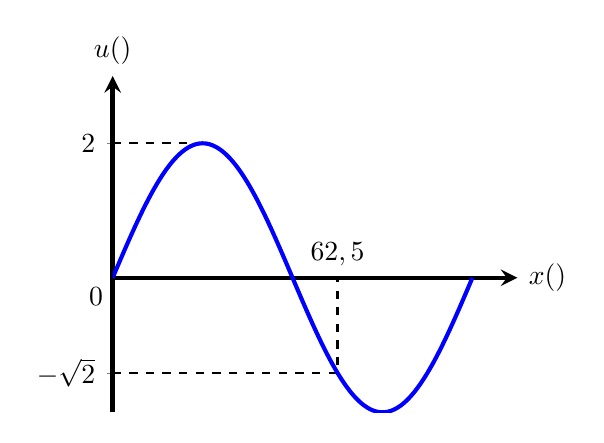
\begin{tikzpicture}  
			\begin{axis}[  ultra thick,scale=0.75,
				xmin=0,  
				xmax=9,  
				ytick={-1.4142,0,2},
				ymin=-2,  
				ymax=3, 
				samples=300,
				xtick=\empty,
				yticklabels={$-\sqrt{2}$,0,2},
				axis lines=center, 
				xlabel=$\xsi{x}{\left(\centi\meter\right)}$, 		ylabel=$\xsi{u}{\left(\si{\centi\meter}\right)}$,
				every axis y label/.style={at=(current axis.above origin),anchor=south},  
				every axis x label/.style={at=(current axis.right of origin),anchor=west},  ]
				\draw[line width=0.8pt, dashed] (0,-1.4142)--(5,-1.4142)--(5,0);
				\draw[line width=0.8pt, dashed] (0,2)--(2,2);
				\addplot [line width=1.5pt, blue, smooth, domain=0:8] {2*cos(deg(pi*x/4-0.5*pi))};  
				\coordinate (O) at (axis cs: 0,0);
				\node[above] at (axis cs: 5,0)  {$62,5$};
			\end{axis}  
			\node[below left] at (O) {0};
	\end{tikzpicture}}
	\shortans[oly]{1000}
	\loigiai{
		$\dfrac{2\pi x}{\lambda}=\pi+\dfrac{\pi}{4}\Rightarrow \lambda=\dfrac{8x}{5}=\dfrac{8\cdot62,5}{5}=\SI{100}{\centi\meter}$.\\
		$v=\lambda f=\SI{1000}{\centi\meter/\second}$.
	}
\end{ex}
% ===============================================================
\begin{ex}
\immini{Trong hiện tượng sóng dừng, xảy ra trên một sợi dây đàn hồi OB. Đồ thị bên là hình ảnh sợi dây tại hai thời điểm $t_1$ và $t_2=t_1+\xsi{\dfrac{1}{3}}{\second}$ (ngay sau đó). Biết rằng tại thời điểm $t_1$, điểm M có vận tốc bằng 0. Tốc độ truyền sóng trên dây bằng bao nhiêu $\si{\centi\meter/\second}$?}
{\vspace{-0.75cm}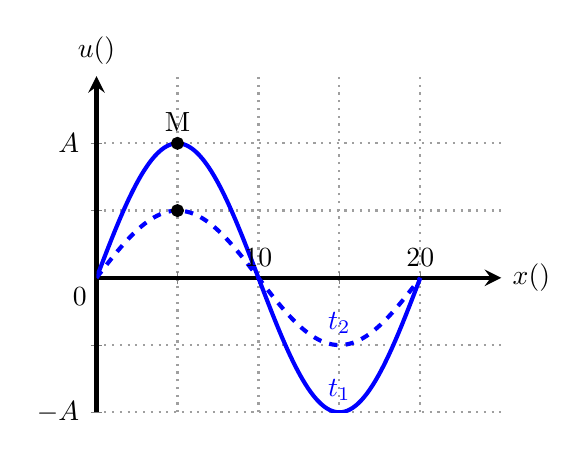
\begin{tikzpicture}  
		\begin{axis}[  ultra thick,scale=0.75,
			xmin=0,  
			xmax=5,  
			xtick={0,1,...,4},
			ytick={-2,-1,1,2},
			ymin=-2,  
			ymax=3, 
			samples=300,
			yticklabels={$-A$,,, $A$},
			xticklabels=\empty,
			axis lines=center, 
			grid style={step=1, line width =0.4pt, color=gray!40!white},
			grid=both, %giới hạn ô lưới
			major grid style={line width=0.8pt,gray!75!white, dotted},
			xlabel=$\xsi{x}{\left(\centi\meter\right)}$, 		ylabel=$\xsi{u}{\left(\si{\centi\meter}\right)}$,
			every axis y label/.style={at=(current axis.above origin),anchor=south},  
			every axis x label/.style={at=(current axis.right of origin),anchor=west},  ]
			\addplot [line width=1.5pt, blue, smooth, domain=0:4] {2*cos(deg(pi*x/2-0.5*pi))} node[above] at(axis cs:3,-2) {$t_1$};  
			\addplot [line width=1.5pt, blue, dashed,smooth, domain=0:4] {1*cos(deg(pi*x/2-0.5*pi))} node[above] at(axis cs:3,-1) {$t_2$};
			\filldraw (axis cs: 1,2) circle(1.5pt) node[above]{M};
			\filldraw (axis cs: 1,1) circle(1.5pt);
			\coordinate (O) at (axis cs: 0,0);
			\node[above] at(axis cs:2,0) {10};
			\node[above] at(axis cs:4,0) {20};
		\end{axis}  
		\node[below left] at (O) {0};
\end{tikzpicture}}
	\shortans[oly]{10}
	\loigiai{
		$t_2-t_1=\dfrac{T}{6}=\xsi{\dfrac{1}{3}}{\second}\Rightarrow T=\SI{2}{\second}$.\\
		$v=\dfrac{\lambda}{T}=\SI{10}{\centi\meter/\second}$.
	}
\end{ex}
\Closesolutionfile{ans}
\begin{center}
	\textbf{--- HẾT ---}
\end{center}
%\part{ĐỀ KIỂM TRA CUỐI HỌC KÌ I LỚP 12}		
%\chapter{ĐỀ 01}
%\input{../data/FINAL-SEM1-001-DA}\newpage
%\begin{tabular}{M{7.5cm}M{10.5cm}}
	\textbf{LỚP CÔ THẢO - THẦY SANG}& \textbf{ĐỀ ÔN TẬP KIỂM TRA CUỐI HỌC KÌ 1}\\
	\textbf{MÃ ĐỀ: 001}& \textbf{Bài thi môn: VẬT LÝ 12}\\
	\textit{(Đề trường THCS-THPT Nguyễn Khuyến năm học 2024 -2025)}& \textit{Thời gian làm bài: 50 phút, không kể thời gian phát đề}
	
	\noindent\rule{4cm}{0.8pt} \\
\end{tabular}
\setcounter{section}{0}
\section{Câu trắc nghiệm nhiều phương án lựa chọn}
\textit{Thí sinh trả lời từ câu 1 đến câu 18. Mỗi câu hỏi thí sinh chọn một phương án}
\setcounter{ex}{0}
\Opensolutionfile{ans}[ans/FINAL-SEM1-001-TN]
% ===================================================================
\begin{ex}
	Nội năng của một vật
	\choice
	{là tổng động năng của các phân tử tạo nên vật}
	{chỉ phụ thuộc vào nhiệt độ của vật}
	{chỉ phụ thuộc vào thể tích của vật}
	{\True phụ thuộc vào thể tích và nhiệt độ của vật}
	\loigiai{}
\end{ex}
% ===================================================================
\begin{ex}
	Chọn câu đúng. Trong quá trình nóng chảy của nước đá đến khi nóng chảy hoàn toàn thì nhiệt độ của nước đá 
	\choice
	{luôn giảm.}
	{\True không thay đổi}
	{luôn tăng}
	{tăng lên sau đó giảm xuống}
	\loigiai{}
\end{ex}
% ===================================================================
\begin{ex}
	Cồn y tế chuyển từ thể lỏng sang thể khí rất nhanh ở điều kiện thông thường. Khi xoa cồn vào da, ta cảm thấy lạnh ở vùng da đó vì
	\choice
	{\True cồn thu nhiệt lượng từ cơ thể qua chỗ da đó để bay hơi}
	{cồn khi bay hơi tỏa nhiệt lượng vào chỗ da đó}
	{cồn khi bay hơi kéo theo lượng nước chỗ da đó ra cơ thể}
	{cồn khi bay hơi tạo ra dòng nước mát chỗ da đó}
	\loigiai{}
\end{ex}
% ===================================================================
\begin{ex}
	Nhiệt hóa hơi riêng có đơn vị đo là
	\choice
	{$\si{J/kg\cdot K}$}
	{$\si{g/mol}$}
	{$\si{mol}$}
	{\True $\si{J/kg}$}
	\loigiai{}
\end{ex}
% ===================================================================
\begin{ex}
	Ở những ngày rất lạnh, nhiều khu vực ở nước ta như Sapa, Mẫu sơn, nước có thể bị đóng băng. Hiện tượng này thể hiện sự chuyển thể nào của chất?
	\choice
	{Sự ngưng tụ}
	{\True Sự đông đặc}
	{Sự nóng chảy}
	{Sự hóa hơi}
	\loigiai{}
\end{ex}
% ===================================================================
\begin{ex}
	Nhiệt hóa hơi riêng là thông tin cần thiết trong việc thiết kế thiết bị nào dưới đây
	\choice
	{\True Tủ lạnh}
	{Máy sấy tóc}
	{Bàn là}
	{Nhiệt kế}
	\loigiai{}
\end{ex}
% ===================================================================
\begin{ex}
	Một lượng khí lí tưởng xác định ở trạng thái có áp suất $p_1$, thể tích $V_1$ và nhiệt độ tuyệt đối $T_1$. Thực hiện quá trình biến đổi lượng khí trên đến trạng thái có áp suất $p_2$, thể tích $V_2$ và nhiệt độ tuyệt đối $T_2$. Phương trình nào sau đây là đúng?
	\choice
	{\True $\dfrac{p_1V_1}{T_1}=\dfrac{p_2V_2}{T_2}$}
	{$\dfrac{p_1}{p_1}=\dfrac{V_1}{V_2}$}
	{$\dfrac{V_1}{V_2}=\dfrac{T_1}{T_2}$}
	{$\dfrac{p_1}{p_2}=\dfrac{T_1}{T_2}$}
	\loigiai{}
\end{ex}
% ===================================================================
\begin{ex}
	Chất nào sau đây có thể tồn tại ở cả ba thể rắn, lỏng, khí ở điều kiện tự nhiên trên trái đất
	\choice
	{Carbon dioxide}
	{Nitrogen}
	{\True Nước}
	{Oxygen}
	\loigiai{}
\end{ex}
% ===================================================================
\begin{ex}
	\immini{Cho một quá trình biến đổi trạng thái của một lượng khí xác định được biểu diễn như hình vẽ. Các thông số trạng thái áp suất p, thể tích V và nhiệt độ tuyệt đối T thay đổi như thế nào khi chuyển từ trạng thái (1) sang trạng thái (2)  
		\choice
		{T không đổi, V tăng và p tăng}
		{\True p tăng, V tăng và T tăng}
		{p tăng, V tăng và T giảm}
		{V không đổi, p tăng và T tăng}} 
	{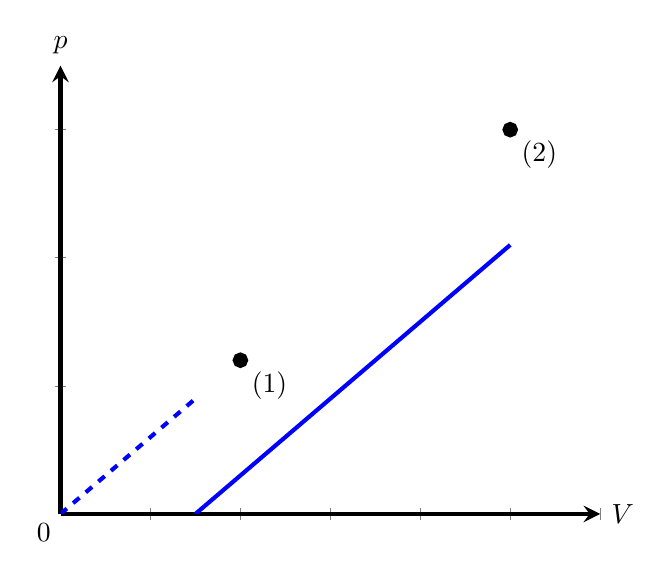
\begin{tikzpicture}  
			\begin{axis}[  ultra thick,
				xmin=0,  
				xmax=12,  
				ymin=0,  
				ymax=7, 
				samples=300,
				yticklabels=\empty,
				xticklabels=\empty,
				axis lines=center, 
				xlabel=$V$, 		ylabel=$p$,
				every axis y label/.style={at=(current axis.above origin),anchor=south},  
				every axis x label/.style={at=(current axis.right of origin),anchor=west},  ]
				\addplot [line width=1.5pt, blue, smooth, dashed, domain=0:3] {0.6*x};  
				\addplot [line width=1.5pt, blue, smooth, domain=3:10] {0.6*(x-3)};
				\filldraw (axis cs: 4,2.4) circle (2pt) node[below right] {(1)};
				\filldraw (axis cs: 10,6) circle (2pt) node[below right] {(2)};
				\coordinate (O) at (axis cs: 0,0);
			\end{axis}  
			\node[below left] at (O) {0};
	\end{tikzpicture}}
	\loigiai{}
\end{ex}
% ===================================================================
\begin{ex}
	Nhiệt nóng chảy riêng của một chất được kí hiệu $\lambda$ và có đơn vị $\dfrac{J}{kg}$. Nhiệt lượng cần thiết để làm nóng chảy hoàn thoàn $\xsi{m}{\left(\kilogram\right)}$ chất đó ở nhiệt độ nóng chảy là 
	\choice
	{$Q=\dfrac{\lambda}{m}$}
	{$Q=(m+\lambda)$}
	{$Q=\dfrac{m}{\lambda}$}
	{\True $Q=m\lambda$}
	\loigiai{}
\end{ex}
% ===================================================================
\begin{ex}
	Chọn phát biểu sai khi nói quá trình đẳng tích (thể tích của khối khí được giữ không đổi) của một lượng khí nhất định.
	\choice
	{\True Tích áp suất và nhiệt độ tuyệt đối là một hằng số}
	{Đồ thị mối liên hệ giữa áp suất và nhiệt độ tuyệt đối có dạng là đường thẳng}
	{Áp suất tỉ lệ thuận với nhiệt độ tuyệt đối}
	{Thương số giữa áp suất và nhiệt độ tuyệt đối là một hằng số}
	\loigiai{}
\end{ex}
% ===================================================================
\begin{ex}
	Câu nào sau đây là sai khi nói về quá trình đẳng nhiệt của một lượng khí nhất định?
	\choice
	{\True Khi áp suất khí tăng 2 lần thì thể tích cũng tăng 2 lần}
	{Đường biểu diễn áp suất theo thể tích là một phần của hyperbol}
	{Tích của áp suất và thể tích luôn không đổi}
	{Áp suất và thể tích tỉ lệ nghịch với nhau}
	\loigiai{}
\end{ex}
% ===================================================================
\begin{ex}
	Ở độ cao 11,5 $\si{km}$ nhiệt độ không khí là $\SI{-56}{\celsius}$ và khối lượng riêng của không khí $\mu = \SI{28.8E-3}{\kg/mol}$. Xem không khó ở độ cao này như khí lí tưởng có hằng số $R=\SI{8.31}{J/mol\cdot K}$. Âp suất khí quyển ở độ cao này là
	\choice
	{$\SI{21.36}{\kPa}$}
	{$\SI{22.80}{\kPa}$}
	{$\SI{21.64}{\kPa}$}
	{\True $\SI{22.54}{\kPa}$}
	\loigiai{$\dfrac{p}{DT}=\dfrac{R}{M}$ \Rightarrow $p\approx \SI{22.54E3}{Pa}$ }
\end{ex}
% ===================================================================
\begin{ex}
	Một khối khí lí tưởng chứa trong một xilanh có pit-tông chuyển động được. Lúc đầu khối khí có thể tích $\SI{18}{\dm^3}$, áp suất $\SI{1.5E5}{\Pa}$. Khối khí được làm lạnh đẳng áp cho đến khi thể tích còn $\SI{18}{\dm^3}$. Bỏ qua ma sát giữa pit-tông và xilanh. Công mà khối khí nhận được là
	\choice
	{$\SI{760}{\J}$}
	{$\SI{580}{\J}$}
	{\True $\SI{600}{\J}$}
	{$\SI{820}{\J}$}
	\loigiai{$A = p(V_1 - V_2) = \SI{600}{\J}$}
\end{ex}
% ===================================================================
\begin{ex}
	\immini{Hình bên là đồ thị biểu diễn sự phụ thuộc của áp suất (p) theo thể tích (V) của một lượng khí lí tưởng xác định khi giữ nhiệt độ không thay đổi. Khi thể tích khối khí là $\SI{0.64}{m^3}$ thì áp suất nhận giá trị nào dưới đây?
		\choice
		{$\SI{18.75}{\kPa}$}
		{\True $\SI{12.5}{\kPa}$}
		{$\SI{15.5}{\kPa}$}
		{$\SI{6.25}{\kPa}$}}
	{\includegraphics[scale=0.6]{../figs/FINAL_SEM1_001_2}}
	\loigiai{$p\cdot 0,64 = 20\cdot 0,4 \Rightarrow p = \SI{12.5}{kPa}$}      
\end{ex}
% ===================================================================
\begin{ex}
	Để mở nút chai bị kẹt, một người dùng cách hơ nóng khí trong chai. Biết rằng khí trong chai lúc chưa hơ nóng có áp suất bằng với áp suất khí quyển và bằng $\SI{1.0E5}{\Pa}$ và nhiệt độ $\SI{8.0}{\celsius}$. Để làm đẩy được nút chai ra cần có chênh lệch áp suất giữa khí trong chai và bên ngoài là $\SI{0.8E5}{\Pa}$. Người này cần hơ để khí trong chai nóng đến nhiệt độ thấp nhất là bao nhiêu ($\si{\celsius}$) để nút chai bật ra. Kết quả làm tròn đến hàng đơn vị.
	\choice
	{265}
	{248}
	{\True 233}
	{235}
	\loigiai{$\dfrac{10^5}{281,15}=\dfrac{1,8 \cdot 10^5}{T_2} \Rightarrow T_2 \approx \SI{506}{\K}$}
\end{ex}
% ===================================================================
\begin{ex}
	Nhiệt nóng chảy riêng của nước đá là $\SI{334E3}{\J/Kg}$. Năng lượng được hấp thụ bởi $\SI{10.0}{\g}$ nước đá để chuyển hoàn toàn từ thể rắn sang thể lỏng là
	\choice
	{$\SI{3.34E2}{\J}$}
	{$\SI{334E3}{\J}$}
	{$\SI{334E2}{\J}$}
	{\True $\SI{3340}{\J}$}
	\loigiai{}
\end{ex}
% ===================================================================
\begin{ex}
	Ở $\SI{27}{\celsius}$ thể tích của một lượng khí lí tưởng là 10,0 lít. Thể tích của lượng khí đó tăng thêm bao nhiêu lít nếu nung nóng đẳng áp để nhiệt độ khối khí tăng thêm $\SI{120}{\celsius}$? 
	\choice
	{3,1 lít}
	{\True 4,0 lít}
	{14,01 lít}
	{1,46 lít}
	\loigiai{}
\end{ex}
\Closesolutionfile{ans}
\section{Câu trắc nghiệm đúng/sai} 
\textit{Thí sinh trả lời từ câu 1 đến câu 4. Trong mỗi ý \textbf{a)}, \textbf{b)}, \textbf{c)}, \textbf{d)} ở mỗi câu, thí sinh chọn đúng hoặc sai}
\setcounter{ex}{0}
\Opensolutionfile{ans}[ans/FINAL-SEM1-001-TF]
% ===================================================================
\begin{ex}
	\immini{Làm thí nghiệm khảo sát mối liên hệ giữa thể tích và nhiệt độ của một lượng khí xác định khi giữ áp suất không đổi. Biết áp kết (1) có mức 0 ứng với áp suất khí quyển, đơn vị đo của áp kế là Bar ($\SI{1}{Bar}=\SI{E5}{Pa}$) ; xilanh (2); pit-tông (3) gắn với tay quay (4); hoopk chứa nước nóng (5) và cảm biến nhiệt (6). Đổ nước nóng vào hộp chứa cho ngập toàn xilanh. Dịch chuyển xilanh từ từ sao cho số chỉ của áp kế không đổi. Kết quả đo giá trị của phần thể tích chứa khí và nhiệt độ sau mỗi phút như bảng bên.}
	{\includegraphics[scale=1]{../figs/FINAL_SEM1_001_3}}
	\choiceTF[t]
	{\True Tỉ số $\dfrac{V}{t+273}$ trong 4 lần đo xấp xỉ bằng nhau, khi đó ta có kết luận $\dfrac{V}{t+273}=$ hằng số}  
	{Đồ thị biểu diễn sự phụ thuộc của thể tích V vào nhiệt độ t (\si{\celsius}) trong hệ trục (OtV) là đường thẳng đi qua gốc tọa độ O}
	{\True Mật độ phân tử trong khí xilanh giảm khi nhiệt độ của khối khí tăng}
	{\True Khi tăng nhiệt độ từ $\SI{32}{\celsius}$ $\SI{32}{\celsius}$ thì thể tích khí tăng thêm xấp xỉ $\SI{20}{\ml}$} 
	\loigiai{
		\begin{itemchoice}
			\itemch Đúng
			\itemch Sai. Nhiệt độ t ($\si{\celsius}$) thì không đi qua gốc tọa độ.
			\itemch Đúng. Khi T tăng thì V tăng mà số phân tử N không đổi nên mật độ phân tử giảm.
			\itemch Đúng. $\dfrac{72}{32+273}=\dfrac{V}{117+273} \Rightarrow V \approx \SI{72}{\ml} \Rightarrow \Delta V = \SI{20}{\ml}$
		\end{itemchoice}
	}
\end{ex}
\begin{ex}
	\immini{Một lượng khí lí tưởng ở trạng thái (1) có áp suất $\SI{4.5E5}{Pa}$, thể tích 1,5 lít và nhiệt độ $\SI{25}{\celsius}$. Khối khí này thực hiện một chu trình biến đổi từ trạng thái (1) đến trạng thái (2) (đường biểu diễn là một phần hyberlbol) rồi đén trạng thái (3), sau đó trở về trạng thái (1) như hình vẽ.}
	{\vspace{-0.5cm}\includegraphics[scale=0.8]{../figs/FINAL_SEM1_001_4}}
	\choiceTF[t]
	{\True Nhiệt độ khối khí ở trạng thái (2) là $\SI{25}{\celsius}$}
	{Từ trạng thái (3) trở về trạng thái (1) là quá trình đẳng áp}
	{\True Thể tích khối khí ở trạng thái (2) là 4,5 lít}
	{Từ trạng thái (2) chuyển đến trạng thái (3) nội năng của khí giảm một lượng $\SI{450}{\J}$}
	\loigiai{
		\begin{itemchoice}
			\itemch Đúng
			\itemch Sai. (3) sang (1) là đẳng tích.
			\itemch Đúng. $4,5 \cdot 10^5 \cdot 1,5 = 1,5 \cdot 10^5 V_2 \Rightarrow V_2 = 4,5l $.
			\itemch Sai. $U_{23}=\dfrac{i}{2}nR(T_2-T_1)=\dfrac{i}{2}\cdot1,5\cdot 10^5 \cdot (1,5-4,5)\cdot 10^{-3}=\dfrac{i}{2}\cdot \SI{450}{\J}$.
			\\ với $i \geq 3 \Rightarrow \Delta U \leq \SI{-675}{\J}$.
		\end{itemchoice}
	}
\end{ex}
\begin{ex}
	Một lốp ô tô được bơm căng không khí ở nhiệt độ $\SI{27}{\celsius}$. Áp suất ban đầu của khí ở áp suất khí quyển thường là $\SI{1.013E5}{Pa}$. Trong quá trình bơm, không khó vào trong lốp bị nén lại và giảm $\SI{75}{\percent}$ thể tích ban đầu (thể tích lượng khí trước khi bơm vào lốp), nhiệt độ khí trong lốp tăng đến $\SI{42}{\celsius}$.
	\choiceTF[t]
	{Trong suốt quá trình bơm, áp suất khí trong lốp xe không đổi}
	{\True Tỉ số thể tích của khí trước khi bơm vào lốp và thể tích sau khi bơm vào lốp là 4}
	{Cần bơm lốp xe với lượng khí lớn nhất để phần diện tích tiếp xúc giữa lốp xe với mặt đường nhỏ nhất, khi đó ma sát giữa lốp xe và mặt đường là nhỏ nhất}
	{\True Khi ô tô chạy với tốc độ cao, nhiệt độ không khí trong lốp tăng đến $\SI{74.6}{\celsius}$ và thể tích lốp thăng thêm $\SI{2}{\percent}$ so với thể tích lốp khi nhiệt độ $\SI{42}{\celsius}$. Áp suất khí trong lốp lúc này là xấp xỉ bằng $\SI{460.3}{kPa}$}
	\loigiai{
		{\includegraphics[scale=2]{../figs/FINAL_SEM1_001_7}}
		\\ $\dfrac{1,013 \cdot 10^5 \cdot V_1}{300,15}=\dfrac{p_2 \cdot 0,25V_1}{315,15}= \dfrac{p_3 \cdot 0,255V_1}{347,75}
		\\ \Rightarrow \begin{cases}
			p_2 \approx \SI{425E3}{\Pa}\\ p_1 \approx \SI{460.3E3}{\Pa}
		\end{cases}$
	}
\end{ex}
\begin{ex}
	Bóng thám không là một thiết bị được sử dụng phổ biến trong ngành khí tượng để thu thập dữ liệu về các thông số thời tiết như nhiệt độ, độ ẩm, áp suất và hướng gió ở độ cao khác nhau của bầu khí quyển. Trên quả bóng có gắn thiết bị gọi là Radiosonde có chức năng ghi nhận các dữ liệu thông qua các cảm biến và phát tín hiệu radio để truyền dữ liệu trở lại mặt đất để các nhà khoa học và nhà khí tượng có thể thu nhập thông tin và phân tích. Bóng thám không thường được làm từ các vật liệu nhẹ có khả năng chịu biến dạng.
	\choiceTF[t]
	{\True Bóng được bơm khí nhẹ như hydrogen hoặc helium}
	{Càng lên cao nhiệt độ của không khí trong bóng càng tăng làm áp suất bóng tăng và bóng sẽ nổ}
	{Bóng thường làm từ các vật liệu nhẹ và có độ bền cao như hợp kim của nhôm hoặc composite}
	{\True Một quả bóng thám không dự báo thời tiết sẽ bị nổ ở áp suất $\SI{0.04}{atm}$ và thể tích tăng lên đến $\SI{542.5}{cm^3}$. Khi ở mặt đất có nhiệt độ $\SI{27}{\celsius}$, bơm khí nhẹ vào bóng với áp suất $\SI{1}{atm}$, thể tích của bóng là $\SI{30}{cm^3}$. Nhiệt độ ở độ cao mà khi bóng nổ là $\SI{-56}{\celsius}$}
	\loigiai{
		\begin{itemchoice}
			\itemch Đúng
			\itemch Sai. Càng lên cao nhiệt độ càng giảm và áp suất bên ngoài cũng giảm. Nhưng áp suất bên ngoài giảm nhanh hơn áp suất bên trong làm bóng nở ra vượt quá giới hạn chịu đựng của vật liệu dẫn đến bóng sẽ nổ.
			\itemch Sai. Bóng thám không thường được làm từ các vật liệu nhẹ có khả năng biến dạng tốt như sao su hoặc latex để bóng có thể giãn nở đến khi lên cao mà không bị nổ sớm.
			\itemch Đúng. $\dfrac{0,04 \cdot 542,5}{T}=\dfrac{1\cdot 30}{27+273} \Rightarrow T \approx \SI{217}{\K} \Rightarrow t \approx \SI{-56}{\celsius} $
		\end{itemchoice}
	}
\end{ex}

\Closesolutionfile{ans}
\section{Câu trắc nghiệm trả lời ngắn} \textit{Thí sinh trả lời từ câu 1 đến câu 6}
\setcounter{ex}{0}
\Opensolutionfile{ans}[ans/FINAL-SEM1-001-TL]
% ===============================================================
\begin{ex}
	Có bao nhiêu kilogam ($\si{\kg}$) khí oxygen (xem là khí lí tưởng) chứa trong bình cầu thể tích $\SI{200}{l}$ ở nhiệt độ $\SI{27}{\celsius}$ và áp suất khí trong bình $\SI{100}{kPa}$. Biết khí oxygen có khối lượng mol $\mu=\SI{32}{\g/mol}$, hằng số khí $R=\SI{8.31}{\J/mol\cdot K}$. Kết quả lấy đến hai chữ số thập phân sau dấu phẩy.
	\shortans[oly]{0,26}
	\loigiai{
		$\dfrac{pV}{T}=\dfrac{m}{M}R \Rightarrow \dfrac{100 \cdot 10^3 \cdot 200 \cdot 10^{-3}}{T} = \dfrac{m}{32 \cdot 10^{-3}}8,31 \Rightarrow m \approx \SI{0.26}{\kg}  $
	}
\end{ex}
\begin{ex}
	Biết nhiệt dung riêng của nước đá và nước lần lượt là $\SI{2100}{\J/Kg}$ và $\SI{4180}{\J/Kg}$, nhiệt nóng chảy riêng của nước đá là $\SI{3.33E5}{\J/kg}$ và nhiệt hóa hơi riêng của nước là $\SI{2.3E6}{\J/kg}$. Nhiệt lượng cần thiết để làm $\SI{2.0}{\g}$ nước đá ở $\SI{-20}{\celsius}$ chuyển hoàn toàn thành hơi nước ở $\SI{100}{\celsius}$ là bao nhiêu kilojun ($\si{kJ}$). Kết quả lấy đến một chữ số thập phân sau dấu phẩy.
	\shortans[oly]{6,2 }
	\loigiai{
		$Q=m(c_d \cdot \Delta t_d + \lambda + c_n \Delta t_n +L)=2 \cdot 10^{-3} \cdot (2100 \cdot 20 + 3,33 \cdot 10^5 + 4180 \cdot 100 + 2,3 \cdot 10^6) = \SI{6186}{\J}$
	}
\end{ex}
\begin{ex}
	\immini{Dùng 1 bơm hút có thể tích xilanh là $\SI{150}{cm^3}$ để hút không khí từ một bình có thể tích $V=\SI{2}{l}$ (kể cả ống nối giữa bơm và bình) chứa không khí ở áp suất $p_0=\SI{E5}{Pa}$. Coi quá trình trên nhiệt độ của khí không thay đổi. Áp suất khí trong bình sau 8 lần hút là bao nhiêu $\si{kPa}$? Kết quả lấy đến một chữ số thập phân sau dấu phẩy.} 
	{\includegraphics[scale=0.7]{../figs/FINAL_SEM1_001_5}}
	\shortans[oly]{56,1 }
	\loigiai{
		$\begin{cases}
			p_0V=p_1\left(V+V_0\right)\\
			p_1V=p_2\left(V+V_0\right)\\
			\dots\\
			p_7V=p_8\left(V+V_0\right)
		\end{cases}$\\
		Nhân các vế rồi rút gọn được $p_0V^8=p_8(V+V_0)^8$
		\\ $10^5 \cdot 2^8 = p_8 \cdot (2+0,15)^8 \Rightarrow p_8 \approx \SI{56070}{\Pa} $
	}
\end{ex}
\begin{ex}
	Một bóng đèn dây tóc có thể tích chứa đầy khí trơ (xem như khí lí tưởng). Khi đèn không hoạt động có nhiệt độ $\SI{27}{\celsius}$, áp suất khí trong bóng đèn là $\SI{1.65}{atm}$ . Khi đèn hoạt động bình thường, nhiệt độ của bóng đèn đạt $\SI{329}{\celsius}$. Áp suất của khối khí trong bóng đèn khi đèn hoạt động bình thường là bao nhiêu? Cho rằng thể tích của bóng đèn không thay đổi theo nhiệt độ. Kết quả lấy đến hai chữ số thập phân sau dấu phẩy.
	\shortans[oly]{3,31}
	\loigiai{
		$\dfrac{1,65}{27+273}=\dfrac{p}{329+273} \Rightarrow p \approx \SI{3.31}{atm}$
	}
\end{ex}
\begin{ex}
	PSI là chỉ số áp suất của không khí bị nén trong lốp xe, được đo bằng đơn vị Pounds trên một Inch vuông (Pounds per Square Inch). PSI thường được ghi trên thành lốp xe, nó cho biết áp suất tối đa mà lốp xe chịu được. Khi bơm hoặc kiểm tra lốp, chúng ta phải làm sao cho lốp đủ hơi, tức là có đủ số PSI cần thiết, thiếu quá hoặc thừa quá đều có thể đưa đến tình trạng hại xe, hư lốp, hao mòn và nguy hiểm nhất là nổ lốp, gây ra tai nạn nghiêm trọng. Một chiếc lốp sau của xe VINFAST chứa không khí ở áp suất 40 Psi (đổi đơn vị $\SI{1}{Psi} \approx \SI{6895}{Pa}$ và nhiệt độ $\SI{27}{\celsius}$. Khi xe chạy nhanh, lốp xe nóng lên làm nhiệt độ không khí trong lốp xe tăng lên tới $\SI{57}{\celsius}$. Áp suất khí trong lốp ở nhiệt độ này là bao nhiêu Psi
	\shortans[oly]{44 }
	\loigiai{
		$\dfrac{40}{27+273}=\dfrac{p}{57+273} \Rightarrow p = \SI{44}{Psi}.$
	}
\end{ex}
\begin{ex}
	\immini{Có một lượng khí helium chứa trong xi lanh đậy kín bởi pít tông (xem như khí lí tưởng) biến đổi chậm từ trạng thái (1) đến trạng thái (2). Hình bên là đường biểu diễn sự phụ thuộc áp suất theo thể tích của khối khí. Khối khí đã nhận một công bằng bao nhiêu kilojun (\si{\kJ}) kể từ lúc bắt đầu biến đổi trạng thái đến lúc đạt nhiệt độ cao nhất.Biết $\SI{1}{atm}$ = \SI{1.013E5}{Pa}. Kết quả lấy đến hai chữ số thập phân sau dấu phẩy.}
	{\vspace{-0.5cm}\includegraphics[scale=1.2]{../figs/FINAL_SEM1_001_6}}
	\shortans[oly]{7,60 }
	\loigiai{
		$p=aV+b\Rightarrow\begin{cases}
			15=10a+b\\
			5=30a+b
		\end{cases}\Rightarrow\begin{cases}
			a=\SI{-0.5}{atm/\liter}\\b=\SI{20}{atm}
		\end{cases}\Rightarrow p=-0,5V+20$\\
		$T_{\max}\Rightarrow pV=\left(-0,5V+20\right)V=-0,5V^2+20V$ đạt max tại $V=\dfrac{20}{2\cdot 0,5}=\SI{20}{\liter}\Rightarrow p=\SI{10}{atm}$\\
		Công khí nhận từ (1) đến khi nhiệt độ cao nhất là diện tích hình thang:
		$$A=\dfrac{1}{2}\left(p_1+p\right)\cdot\left(V_1-V\right)\approx\SI{7.60E3}{\joule}=\SI{7.60}{\kilo\joule}.$$
		
	}
\end{ex}

\Closesolutionfile{ans}
\begin{center}
	\textbf{--- HẾT ---}
\end{center}
%\chapter{ĐỀ 02}
%\input{../data/FINAL-SEM1-002-DA}\newpage
%\begin{tabular}{M{6.5cm}M{11cm}}
	\textbf{TRUNG TÂM MANABIE}& \textbf{ĐỀ ÔN TẬP KIỂM TRA CUỐI HỌC KÌ 1}\\
	\textbf{MÃ ĐỀ: 002}& \textbf{Bài thi môn: VẬT LÝ 12}\\
	\textit{(Đề trường THPT Lương Thế Vinh - Hà Nội năm học 2024 -2025)}& \textit{Thời gian làm bài: 50 phút, không kể thời gian phát đề}
	
	\noindent\rule{4cm}{0.8pt} \\
\end{tabular}
\setcounter{section}{0}
\section{Câu trắc nghiệm nhiều phương án lựa chọn}
\textit{Thí sinh trả lời từ câu 1 đến câu 18. Mỗi câu hỏi thí sinh chọn một phương án}
\setcounter{ex}{0}
\Opensolutionfile{ans}[ans/FINAL-SEM1-002-TN]
% ===================================================================
\begin{ex}
	Trong các chất sau, chất nào \textbf{không phải} là chất rắn kết tinh
	\choice
	{muối ăn}
	{\True thủy tinh}
	{kim cương}
	{thạch anh}
	\loigiai{}
\end{ex}
% ===================================================================
\begin{ex}
	Đặc điểm nào sau đây là đặc điểm của thể lỏng?
	\choice
	{Khoảng cách giữa các phân tử rất lớn so với kích thước của chúng}
	{\True Lực tương tác phân tử yếu hơn lực tương tác phân tử ở thể rắn}
	{Không có thể tích và hình dạng riêng xác định}
	{Các phân tử dao động xung quanh vị trí cân bằng xác định}
	\loigiai{}
\end{ex}
% ===================================================================
\begin{ex}
	Khi quan sát sự nóng chảy của nước đá tại nhiệt độ nóng chảy, trong suốt thời gian nóng chảy thì
	\choice
	{nhiệt độ của nước đá tăng}
	{nhiệt độ của nước đá giảm}
	{\True nhiệt độ của nước không thay đổi}
	{nhiệt độ của nước đá ban đầu tăng sau đó giảm}
	\loigiai{}
\end{ex}
% ===================================================================
\begin{ex}
	Sử dụng hai nhiệt kế rượu có độ chia từ $\SI{0}{\celsius}$ tới $\SI{100}{\celsius}$, hình vẽ nào trong hình bên dưới phù hợp với trường hợp nhiệt kế 1 được đặt vào một cốc đựng nước nóng còn nhiệt kế 2 được đặt vào một cốc nước lạnh?
	\begin{center}
		\includegraphics[scale=0.7]{../figs/FINAL-SEM1-002-1}
	\end{center}
	\choice
	{Hình B}
	{Hình C}
	{Hình A}
	{\True Hình D}
	\loigiai{}
\end{ex}
% ===================================================================
\begin{ex}
	\immini{Hiện tượng quả bóng bàn bị móp (nhưng chưa bị thủng) khi thả vào cốc nước nóng sẽ phồng trở lại là do nội năng của chất khí bên trong quả bóng}	
	{\vspace{-0.5cm}\includegraphics[scale=0.5]{../figs/FINAL-SEM1-002-2}}
	\choice
	{\True tăng lên}
	{giảm xuống}
	{không thay đổi}
	{giảm đi hai lần}
	\loigiai{}
\end{ex}
% ===================================================================
\begin{ex}
	Theo định luật I nhiệt động lực học $\Delta U=Q+A$. Biểu thức nào sau đây diễn tả quá trình biến thiên nội năng khi hệ nhận công và truyền nhiệt
	\choice
	{$\Delta U=Q+A$ với $Q>0$ và $A>0$}
	{$\Delta U=Q+A$ với $Q>0$ và $A<0$}
	{\True $\Delta U=Q+A$ với $Q<0$ và $A>0$}
	{$\Delta U=Q+A$ với $Q<0$ và $A<0$}
	\loigiai{}
\end{ex}
% ===================================================================
\begin{ex}
	Biết nhiệt nóng chảy riêng của nước đá là $\lambda=\SI{3.4E5}{\joule/\kilogram}$. Nhiệt lượng $Q$ cần cung cấp để làm nóng chảy $\SI{200}{\gram}$ nước đá ở $\SI{0}{\celsius}$ bằng
	\choice
	{$\SI{0.34E3}{\joule}$}
	{$\SI{340E5}{\joule}$}
	{$\SI{68E7}{\joule}$}
	{\True $\SI{68E3}{\joule}$}
	\loigiai{}
\end{ex}
% ===================================================================
\begin{ex}
	Biết nhiệt hóa hơi riêng của nước là $L=\SI{2.3E6}{\joule/\kilogram}$. Nhiệt lượng cần cung cấp để làm bay hơi hoàn toàn $\SI{300}{\gram}$ nước ở $\SI{100}{\celsius}$ là 
	\choice
	{$\SI{69E6}{\joule}$}
	{\True $\SI{6.9E5}{\joule}$}
	{$\SI{2.3E6}{\joule}$}
	{$\SI{0.23E4}{\joule}$}
	\loigiai{}
\end{ex}
% ===================================================================
\begin{ex}
\immini{Đồ thị biểu diễn hai đường đẳng nhiệt của cùng một lượng khí lí tưởng biểu diễn như hình vẽ. Mối quan hệ về nhiệt độ của hai đường đẳng nhiệt này là
	\choice
	{\True $T_2>T_1$}
	{$T_2=T_1$}
	{$T_2<T_1$}
	{$T_2\le T_1$}}
{\vspace{-0.5cm}	\includegraphics[scale=0.4]{../figs/FINAL-SEM1-002-3}}
	\loigiai{}
\end{ex}
% ===================================================================
\begin{ex}
	Một lượng khí có áp suất $\SI{750}{\milli\meter Hg}$, nhiệt độ $\SI{37}{\celsius}$ và thể tích $\SI{70}{\centi\meter^3}$. Thể tích khí ở điều kiện tiêu chuẩn (nhiệt độ $\SI{0}{\celsius}$ và áp suất $\SI{760}{\milli\meter Hg}$) có giá trị gần bằng
	\choice
	{$\SI{22.4}{\centi\meter^3}$}
	{$\SI{32.7}{\centi\meter^3}$}
	{\True $\SI{60.8}{\centi\meter^3}$}
	{$\SI{78}{\centi\meter^3}$}
	\loigiai{
	$\dfrac{p_1V_1}{T_1}=\dfrac{p_2V_2}{T_2}\Leftrightarrow\dfrac{750\cdot70}{37+273}=\dfrac{760V}{273}\Rightarrow V\approx\SI{60.8}{\centi\meter^3}$.
	}
\end{ex}
% ===================================================================
\begin{ex}
Gọi $p$ là áp suất khối khí, $\mu$ là mật độ của phân tử khí, $m$ là khối lượng của phân tử khí, $\overline{v^2}$ là trung bình của bình phương tốc độ, $k$ là hằng số Boltzmann, $T$ là nhiệt độ tuyệt đối. Công thức nào sau đây mô tả đúng mối liên hệ giữa các đại lượng?	
	\choice
	{$p=\dfrac{2}{3}\mu m\overline{v^2}$}
	{$p=3\mu kT$}
	{\True $p=\mu kT$}
	{$p=\dfrac{3}{2}\mu m\overline{v^2}$}
	\loigiai{}
\end{ex}
% ===================================================================
\begin{ex}
Động năng tịnh tiến trung bình của phân tử khí lí tưởng ở $\SI{37}{\celsius}$ có giá trị là	
	\choice
	{$\SI{5.21E-22}{\joule}$}
	{\True $\SI{6.42E-21}{\joule}$}
	{$\SI{6.24E23}{\joule}$}
	{$\SI{5.12E23}{\joule}$}
	\loigiai{
	$W_{\text{đ}}=\dfrac{3}{2}kT=\SI{6.42E-21}{\joule}.$
	}
\end{ex}
% ===================================================================
\begin{ex}
	Hình vẽ nào dưới đây biểu diễn đúng hướng của vector cảm ứng từ tại M gây ra bởi dòng điện trong dây dẫn thẳng dài vô hạn?
	\choice
	{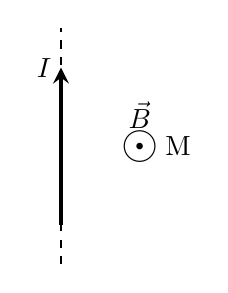
\begin{tikzpicture}
			\draw[dashed] (0,0)--(0,3);
			\draw[-stealth, line width=1.5pt] (0,0.5)--(0,2.5);
			\node at (1,1.5) {\LARGE $\odot$};
			\node[above] at (1,1.6) {$\vec{B}$};
			\node[left] at (0,2.5) {$I$};
			\node[right] at (1.2,1.5) {M};
	\end{tikzpicture}}
	{\True 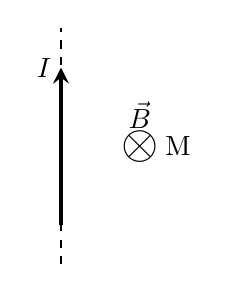
\begin{tikzpicture}
			\draw[dashed] (0,0)--(0,3);
			\draw[-stealth, line width=1.5pt] (0,0.5)--(0,2.5);
			\node at (1,1.5) {\LARGE $\otimes$};
			\node[above] at (1,1.6) {$\vec{B}$};
			\node[left] at (0,2.5) {$I$};
			\node[right] at (1.2,1.5) {M};
	\end{tikzpicture}}
	{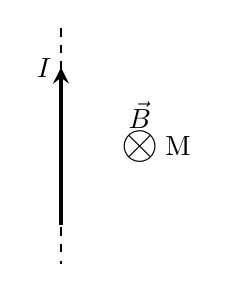
\begin{tikzpicture}
			\draw[dashed] (0,3)--(0,0);
			\draw[-stealth, line width=1.5pt] (0,0.5)--(0,2.5);
			\node at (1,1.5) {\LARGE $\otimes$};
			\node[above] at (1,1.6) {$\vec{B}$};
			\node[left] at (0,2.5) {$I$};
			\node[right] at (1.2,1.5) {M};
	\end{tikzpicture}}
	{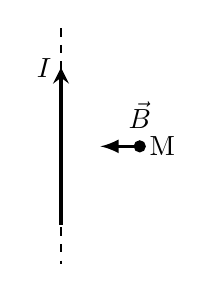
\begin{tikzpicture}
			\draw[dashed] (0,3)--(0,0);
			\draw[-stealth, line width=1.5pt] (0,0.5)--(0,2.5);
			\draw[-latex, line width=1.25pt] (1,1.5)--(0.5,1.5);
			\node[above] at (1,1.6) {$\vec{B}$};
			\node[left] at (0,2.5) {$I$};
			\filldraw (1,1.5) circle (2pt) node[right]{M};
	\end{tikzpicture}}
	\loigiai{}
\end{ex}
% ===================================================================
\begin{ex}
Hình nào sau đây biểu diễn không đúng vector lực từ tác dụng đoạn dây dẫn mang dòng điện đặt trong từ trường đều	
\begin{center}
	\begin{tabular}{M{4cm}M{4cm}M{4cm}M{4cm}}
		\begin{tikzpicture}
			\coordinate(A) at(0.2,0.2);
			\coordinate(B) at($(A)+(30:2.5)$);
			\foreach \x in {0,2}{
				\foreach \y in {0,2}{
					\node at (\x,\y) {\LARGE$\otimes$};
				}
			};
			\draw[-stealth, line width=1.5pt, blue] ($(A)!0.5!(B)$)--+(120:1.5);
			\draw[line width=4pt, gray,decoration={markings, mark=at position 0.5 with {\arrow{stealth}}},
			postaction={decorate}] (A)--(B);
			\node[below] at ($(A)!0.5!(B)$) {$I$};
			\node[right, blue] at ($(A)!0.5!(B)+(120:1.5)$) {$\vec{F}$};
			\node[right] at (2.1,2) {$\vec{B}$};
		\end{tikzpicture}
		&
		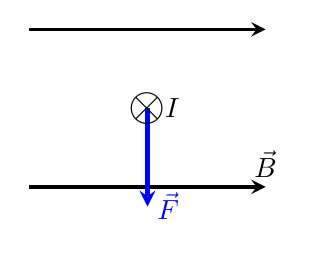
\begin{tikzpicture}
			\draw[-stealth, line width=1.25pt] (0,0)--(3,0);
			\draw[-stealth, line width=1.25pt] (0,2)--(3,2);
			\draw[-stealth, blue, line width=1.5pt] (1.5,1)--(1.5,-0.25);
			\node at(1.5,1) {\LARGE$\otimes$};
			\node[right] at(1.6,1) {$I$};
			\node[right, blue] at(1.5,-0.25) {$\vec{F}$};
			\node[above] at(3,0) {$\vec{B}$};
		\end{tikzpicture}
		&
		\begin{tikzpicture}
			\draw[-stealth, line width=1.25pt] (0,0)--(3,0);
			\draw[-stealth, line width=1.25pt] (0,2)--(3,2);
			\draw[-stealth, blue, line width=1.5pt] (1.5,1)--(1.5,2.25);
			\draw[line width=4pt, gray,decoration={markings, mark=at position 0.5 with {\arrow{stealth}}},
			postaction={decorate}] (0.5,1)--(2.5,1);
			\node[below] at(1.6,1) {$I$};
			\node[right, blue] at(1.5,2.25) {$\vec{F}$};
			\node[above] at(3,0) {$\vec{B}$};
		\end{tikzpicture}
		&
		\begin{tikzpicture}
			\coordinate(A) at (0.2,-0.2);
			\coordinate(B) at ($(A)+(-30:2.5)$);
			\draw[-stealth, line width=1.25pt] (0,0)--(0,-2);
			\draw[-stealth, line width=1.25pt] (2.5,0)--(2.5,-2);
			\draw[line width=4pt, gray,decoration={markings, mark=at position 0.5 with {\arrow{stealth}}},
			postaction={decorate}] (A)--(B);
			\node[above] at($(A)!0.5!(B)+(0,0.1)$) {$I$};
			\node[below, blue] at($(A)!0.5!(B)-(0,0.2)$) {$\vec{F}$};
			\node[above] at(3,0) {$\vec{B}$};
			\node[fill=none] at ($(A)!0.5!(B)$) {\LARGE$\otimes$};
		\end{tikzpicture}\\
		\textbf{Hình 1} & \textbf{Hình 2} & \textbf{Hình 3} & \textbf{Hình 4}
	\end{tabular}
\end{center}
	\choice
	{Hình 1}
	{Hình 2}
	{\True Hình 3}
	{Hình 4}
	\loigiai{}
\end{ex}
% ===================================================================
\begin{ex}
Một quả bóng có dung tích $\SI{2.5}{\liter}$. Người ta bơm không khí ở áp suất $\SI{E5}{\pascal}$ vào bóng. Mỗi lần bơm được $\SI{150}{\centi\meter^3}$ không khí. Tính áp suất của không khí trong quả bóng sau 50 lần bơm. Coi quả bóng trước khi bơm không có không khí và nhiệt độ trong quả bóng không thay đổi.
	\choice
	{$\SI{25E5}{\pascal}$}
	{$\SI{2.5E5}{\pascal}$}
	{$\SI{0.25E5}{\pascal}$}
	{\True $\SI{3E5}{\pascal}$}
	\loigiai{
	$p_1V_1=p_2V_2\Leftrightarrow10^5\cdot0,15\cdot50=2,5p\Rightarrow p=\SI{3E5}{\pascal}$.
	}
\end{ex}
% ===================================================================
\begin{ex}
	Ba chất lỏng không tác dụng hóa học với nhau và được trộn lẫn vào nhau trong một nhiệt lượng kế; chúng có khối lượng lần lượt là $m_1=\SI{1}{\kilogram}$, $m_2=\SI{10}{\kilogram}$, $m_3=\SI{5}{\kilogram}$ có nhiệt dung riêng lần lượt là $c_1=\SI{2000}{\kilogram\cdot\kelvin}$; $c_2=\SI{4000}{\joule/\kilogram\cdot\kelvin}$; $c_3=\SI{2500}{\joule/\kilogram\cdot\kelvin}$ và có nhiệt độ là $t_1=\SI{6}{\celsius}$; $t_2=\SI{20}{\celsius}$; $t_3=\SI{-60}{\celsius}$. Bỏ qua sự trao đổi nhiệt với nhiệt lượng kế và với môi trường. Nhiệt độ của hỗn hợp khi xảy ra cân bằng nhiệt xấp xỉ
	\choice
	{$\SI{-2.5}{\celsius}$}
	{$\SI{-1.9}{\celsius}$}
	{\True $\SI{1.1}{\celsius}$}
	{$\SI{3.5}{\celsius}$}
	\loigiai{
	$t_{\text{cb}}=\dfrac{m_1c_1t_1+m_2c_2t_2+m_3c_3t_3}{m_1c_1+m_2c_2+m_3c_3}\approx\SI{1.1}{\celsius}$.
	}
\end{ex}
% ===================================================================
\begin{ex}
	Khí helium có khối lượng mol phân tử là $\SI{4}{\gram/\mole}$. Coi các phân tử khí là giống nhau. Trung bình của bình phương tốc độ trong chuyển động nhiệt của phân tử khí helium ở nhiệt độ $\SI{320}{\kelvin}$ là
	\choice
	{$\SI{1.995E6}{\meter^2/\second^2}$}
	{$\SI{2.01E6}{\meter^2/\second^2}$}
	{$\SI{2010}{\meter^2/\second^2}$}
	{$\SI{2020}{\meter^2/\second^2}$}
	\loigiai{
	$\overline{v^2}=\dfrac{3RT}{M}\approx\SI{1.995E6}{\meter^2/\second^2}$.
	}
\end{ex}
% ===================================================================
\begin{ex}
	Treo đoạn dây dẫn có chiều dài $\ell=\SI{10}{\centi\meter}$, khối lượng $m=\SI{5}{\gram}$ bằng hai dây mảnh, nhẹ sao cho dây dẫn nằm ngang. Biết cảm ứng từ của từ trường hướng thẳng đứng xuống dưới, có độ lớn $B=\SI{0.5}{\tesla}$ và dòng điện đi qua dây dẫn là $I=\SI{1}{\ampere}$. Lấy $g=\SI{10}{\meter/\second^2}$ thì góc lệch của dây treo so với phương thẳng đứng là
	\choice
	{$\SI{30}{\degree}$}
	{\True $\SI{45}{\degree}$}
	{$\SI{60}{\degree}$}
	{$\SI{90}{\degree}$}
	\loigiai{
	$\tan\alpha=\dfrac{F}{P}=\dfrac{ILB}{mg}=1\Rightarrow \alpha=\SI{45}{\degree}$.
	}
\end{ex}
\Closesolutionfile{ans}
\section{Câu trắc nghiệm đúng/sai} 
\textit{Thí sinh trả lời từ câu 1 đến câu 4. Trong mỗi ý \textbf{a)}, \textbf{b)}, \textbf{c)}, \textbf{d)} ở mỗi câu, thí sinh chọn đúng hoặc sai}
\setcounter{ex}{0}
\Opensolutionfile{ans}[ans/FINAL-SEM1-002-TF]
% ===================================================================
\begin{ex}
	\immini{Cho đồ thị biểu diễn sự thay đổi nhiệt độ của nước theo thời gian đun như hình bên. Biết nhiệt độ nóng chảy của nước đá là $\SI{0}{\celsius}$, nhiệt độ sôi của nước là $\SI{100}{\celsius}$.
	\choiceTF[t]
	{\True Từ phút thứ 0 đến phút thứ 5 nước ở thể rắn}
	{\True Từ phút thứ 5 đến phút thứ 10 xảy ra quá trình nóng chảy}
	{Từ phút thứ 10 đến phút thứ 25 nước ở thể rắn}
	{\True Từ phút thứ 25 đến phút thứ 30 xảy ra quá trình sôi}
	}
	{\begin{tikzpicture}  
			\begin{axis}[  ultra thick,scale=0.65,
				xmin=0,  
				xmax=34,  
				xtick={0,5,...,35},
				ytick={-10,0,...,120},
				minor x tick num=1,
				minor y tick num=0,
				ymin=-10,  
				ymax=110, 
				samples=300,
				yticklabels=\empty,
				axis lines=center, 
				grid style={step=1, line width=0.8pt,gray!60!white},
				grid=both, %giới hạn ô lưới
				major grid style={line width=0.8pt,gray!60!white},
				xlabel=$\xsi{t}{\left(\minute\right)}$, 		
				ylabel=$\text{Nhiệt độ}\ \left(\si{\celsius}\right)$,
				every axis y label/.style={at=(current axis.above origin),anchor=south},  
				every axis x label/.style={at=(current axis.right of origin),anchor=south},  ]
				\coordinate (A) at (axis cs: 0,-10);
				\coordinate (B) at (axis cs: 5,0);
				\coordinate (C) at (axis cs: 10,0);
				\coordinate (D) at (axis cs: 25,100);
				\coordinate (E) at (axis cs: 30,100);
				\draw[line width=1.5pt,blue] plot coordinates {(A) (B) (C) (D) (E)};
				\coordinate (O) at (axis cs: 0,0);
				\coordinate (t1) at (axis cs: 0,-10);
				\coordinate (t2) at (axis cs: 0,100);
			\end{axis}  
			\node[left] at (O) {0};
			\node[left] at (t1) {$-10$};
			\node[left] at (t2) {$100$};
	\end{tikzpicture}}
	
	\loigiai{}
\end{ex}
% ===================================================================
\begin{ex}
\immini{Cung cấp nhiệt lượng $\SI{2.5}{\joule}$ cho một khối khí lí trong một xilanh đặt nằm ngang như hình vẽ. Chất khí nở ra đẩy pít-tông đi một đoạn $\SI{5.0}{\centi\meter}$. Biết lực ma sát giữa pít-tông và xilanh có độ lớn là $\SI{20.0}{\newton}$, diện tích tiết diện của pít-tông là $\SI{2.0}{\centi\meter^2}$. Coi pít-tông chuyển động thẳng đều và áp suất bên phải pít-tông bằng 0. Trong các phát biểu sau, phát biểu nào đúng, phát biểu nào sai?}
{\includegraphics[scale=0.7]{../figs/FINAL-SEM1-002-4}}
	\choiceTF[t]
	{\True Công của khối khí thực hiện là $\SI{1.0}{\joule}$}
	{Độ biến thiên nội năng của khối khí là $\SI{0.50}{\joule}$}
	{\True Trong quá trình dãn nở, áp suất của chất khí là $\SI{1.0E5}{\pascal}$}
	{Thể tích khí trong xilanh tăng $\SI{5.0}{\liter}$}
	\loigiai{
	\begin{itemchoice}
		\itemch Đúng. $A'=Fs=\SI{1}{\joule}$.
		\itemch Sai. $\Delta U=Q-A'=\SI{1.5}{\joule}$.
		\itemch Đúng. $p=\dfrac{F}{S}=\SI{E5}{\pascal}$.
		\itemch Sai. $A'=p\Delta V\Rightarrow \Delta V=\SI{0.01}{\liter}$.
	\end{itemchoice}
	}
\end{ex}
% ===================================================================
\begin{ex}
	Một hệ làm nóng nước bằng năng lượng mặt trời có hiệu suất chuyển đổi $\SI{25}{\percent}$; cường độ bức xạ mặt trời lên bộ thu nhiệt là $\SI{1000}{\watt/\meter^2}$; diện tích bộ thu là $\SI{5}{\meter^2}$. Cho nhiệt dung riêng của nước là $\SI{4200}{\joule/\kilogram\cdot\kelvin}$.
	\choiceTF[t]
	{\True Công suất bức xạ chiếu lên bộ thu nhiệt là $\SI{5000}{\watt}$}
	{\True Trong $\SI{1.00}{\hour}$, năng lượng mặt trời chiếu lên bộ thu nhiệt là $\SI{18}{\mega\joule}$}
	{Trong $\SI{1.00}{\hour}$, phần năng lượng chuyển thành năng lượng nhiệt là $\SI{5}{\mega\joule}$}
	{Nếu hệ thống đó làm nóng $\SI{30.0}{\kilogram}$ nước thì trong khoảng thời gian $\SI{1.00}{\hour}$ nhiệt độ của nước tăng thêm $\SI{30}{\celsius}$}
	\loigiai{\begin{itemchoice}
			\itemch Đúng. $\calP=IS=\SI{5}{\kilo\watt}$.
			\itemch Đúng. $A=\calP t=\SI{18}{\mega\joule}$.
			\itemch Sai. $Q=HA=\SI{4.5}{\mega\joule}$.
			\itemch Sai. $\Delta t=\dfrac{Q}{mc}=\SI{35.7}{\celsius}$.
	\end{itemchoice}}
\end{ex}
% ===================================================================
\begin{ex}
	Có $\SI{16}{\gram}$ khí oxygen ở nhiệt độ $\SI{27}{\celsius}$, áp suất $\SI{3E5}{\pascal}$. Sau khi đun nóng đẳng áp, khối khí có thể tích là $\SI{10}{\liter}$. Biết khối lượng mol phân tử của khí oxygen là $\SI{32}{\gram/\mole}$ và hằng số khí lí tưởng $R=\SI{8.31}{\joule/\mole\cdot\kelvin}$.
	\choiceTF[t]
	{Thể tích của khối khí trước khi đun nóng là $\SI{4.5}{\liter}$}
	{\True Khối lượng riêng của lượng khí trên trước khi đun nóng xấp xỉ $\SI{3.85}{\kilogram/\meter^3}$}
	{\True Nhiệt độ của khối khí sau khi đun nóng xấp xỉ $\SI{722}{\kelvin}$}
	{Nếu tiếp tục đun nóng khối khí đến nhiệt độ $\SI{477}{\celsius}$ và giữ nguyên thể tích khí là $\SI{10}{\liter}$. Áp suất chất khí lúc này là $\SI{7.5E3}{\pascal}$}
	\loigiai{
	\begin{itemchoice}
		\itemch Sai. $pV=\dfrac{m}{M}RT\Rightarrow V\approx\SI{4.157E-3}{\meter^3}=\SI{4.157}{\liter}$.
		\itemch Đúng. $\rho=\dfrac{m}{V}=\SI{3.85}{\kilogram/\meter^3}$.
		\itemch Đúng. 
		\itemch Sai. Khi tăng nhiệt độ và giữ nguyên thể tích thì áp suất khí tăng $p>\SI{3E5}{\pascal}$.
	\end{itemchoice}
	}
\end{ex}
\Closesolutionfile{ans}
\section{Câu trắc nghiệm trả lời ngắn} \textit{Thí sinh trả lời từ câu 1 đến câu 6}
\setcounter{ex}{0}
\Opensolutionfile{ans}[ans/FINAL-SEM1-002-TL]
% ===============================================================
\begin{ex}
	Một đoạn dây dẫn dài $\SI{20}{\centi\meter}$ được đặt trong từ trường đều và vuông góc với vector cảm ứng từ. Dòng điện qua dây dẫn có cường độ $\SI{0.5}{\ampere}$. Lực từ tác dụng lên đoạn dây dẫn này là  $F=\SI{0.002}{\newton}$. Xác định độ lớn cảm ứng từ $B$ của từ trường theo đơn vị tesla $\left(\si{\tesla}\right)$.
	\shortans[oly]{0,02}
	\loigiai{
		$B=\dfrac{F}{IL}=\SI{0.02}{\tesla}$.
	}
\end{ex}
% ===============================================================
\begin{ex}
	Một lượng khí lí tưởng có thể tích $\SI{2.1}{\liter}$ và áp suất $\SI{1}{atm}$. Người ta nén đẳng nhiệt khí tới áp suất $\SI{3}{atm}$. Thể tích của khí sau khi nén là bao nhiêu lít?
	\shortans[oly]{0,7}
	\loigiai{
		$p_1V_1=p_2V_2\Leftrightarrow 1\cdot2,1=3\cdot V_2\Rightarrow V_2=\SI{0.7}{\liter}$.
	}
\end{ex}
% ===============================================================
\begin{ex}
	Có $\SI{0.5}{\liter}$ nước ở nhiệt độ $\SI{30}{\celsius}$, nhiệt lượng tổng cộng cần cung cấp để nó biến hoàn toàn thành hơi ở nhiệt độ sôi $\SI{100}{\celsius}$ là bao nhiêu $\si{\kilo\joule}$. Biết nhiệt dung riêng của nước là $\SI{4200}{\joule/\kilogram\cdot\kelvin}$ và khối lượng riêng $\rho=\SI{E3}{\kilogram/\meter^3}$, nhiệt hóa hơi riêng của nước là $\SI{2.3E6}{\joule/\kilogram}$.
	\shortans[oly]{1297}
	\loigiai{
		$m=V\rho=\SI{0.5}{\kilogram}$.\\
		$Q=mc\Delta t+mL=\SI{1297}{\kilo\joule}$.
	}
\end{ex}
% ===============================================================
\begin{ex}
	Vào những ngày trời nắng nóng, nhiệt độ không khí ngoài sân là $\SI{45}{\celsius}$, trong khi nhiệt độ không khí trong nhà là $\SI{27}{\celsius}$. Giả sử áp suất không khí trong nhà và ngoài sân là như nhau. Khối lượng riêng của không khí trong nhà lớn hơn khối lượng riêng của không khí ngoài sân bao nhiêu lần?
	\shortans[oly]{1,06}
	\loigiai{
		$pV=\dfrac{m}{M}RT\Rightarrow\rho=\dfrac{pM}{RT}$.\\
		$\Rightarrow \dfrac{\rho_2}{\rho_1}=\dfrac{T_1}{T_2}=\dfrac{45+273}{27+273}\approx1,06$.
	}
\end{ex}
% ===============================================================
\begin{ex}
	\immini{Một bình thủy tinh hình trụ, tiết diện $\SI{100}{\centi\meter^2}$ chứa khí lí tưởng bị chặn với tấm chắn có khối lượng không đáng kể, áp suất, nhiệt độ, chiều cao của cột không khí bên trong bình lần lượt là $\SI{1}{atm}$, $\SI{30}{\celsius}$ và $\SI{60}{\centi\meter}$. Đặt lên tấm chắn vật có trọng lượng $\SI{500}{\newton}$, cột khí bên trong có chiều cao $\SI{30}{\centi\meter}$. Nhiệt độ của khí bên trong bình là bao nhiêu độ $\si{\kelvin}$ (làm tròn đến hàng đơn vị).}
	{\includegraphics[scale=0.4]{../figs/FINAL-SEM1-002-5}}
	\shortans[oly]{226}
	\loigiai{
		\begin{center}
			\begin{tabular}{|M{5cm}|M{5cm}|M{5cm}|}
				\hline
			$p$&$V$ & $T$\\
			\hline
			$p_0=\SI{101325}{\pascal}$ & $60S$ & $30+273=\SI{303}{\kelvin}$\\
			\hline
			$p_0+\dfrac{F}{S}=\SI{151325}{\pascal}$ & $30S$ & $T_2$\\
			\hline
			\end{tabular}
		\end{center}
		$$\dfrac{p_1V_1}{T_1}=\dfrac{p_2V_2}{T_2}\Rightarrow T_2=\SI{226}{\kelvin}.$$
	}
\end{ex}
% ===============================================================
\begin{ex}
\immini{	Có ba bình thể tích $V_1=V$, $V_2=2V$, $V_3=3V$, thông với nhau nhưng cách nhiệt đối với nhau và với môi trường bên ngoài. Ban đầu các bình chứa khí ở cùng nhiệt độ $T_0$ và áp suất $p_0=\SI{1}{atm}$. Người ta giữ nguyên nhiệt độ bình 1, nâng nhiệt độ  bình 2 lên $2T_0$ và bình 3 lên $3T_0$. Áp suất mới trong các bình bằng bao nhiêu $\si{atm}$?}
{\includegraphics[scale=0.4]{../figs/FINAL-SEM1-002-6}}
	\shortans[oly]{2}
	\loigiai{
		$n=n_1+n_2+n_3\Leftrightarrow \dfrac{p_06V}{T_0}=\dfrac{pV}{T_0}+\dfrac{p\cdot 2V}{2T_0}+\dfrac{p\cdot 3V}{3T_0}\Rightarrow p=\SI{2}{atm}.$
	}
\end{ex}
\Closesolutionfile{ans}
\begin{center}
	\textbf{--- HẾT ---}
\end{center}

%\chapter{ĐỀ 03}
%\input{../data/FINAL-SEM1-003-DA}\newpage
%\begin{tabular}{M{6.5cm}M{11cm}}
	\textbf{TRUNG TÂM MANABIE}& \textbf{ĐỀ ÔN TẬP KIỂM TRA CUỐI HỌC KÌ 1}\\
	\textbf{MÃ ĐỀ: 003}& \textbf{Bài thi môn: VẬT LÝ 12}\\
	\textit{(Đề trường THPT Thuận Thành số 1 - Bắc Ninh năm học 2024 -2025)}& \textit{Thời gian làm bài: 50 phút, không kể thời gian phát đề}
	
	\noindent\rule{4cm}{0.8pt} \\
\end{tabular}
\setcounter{section}{0}
\section{Câu trắc nghiệm nhiều phương án lựa chọn}
\textit{Thí sinh trả lời từ câu 1 đến câu 18. Mỗi câu hỏi thí sinh chọn một phương án}
\setcounter{ex}{0}
\Opensolutionfile{ans}[ans/FINAL-SEM1-003-TN]
% ===================================================================
\begin{ex}
	Gọi $p$, $V$, $T$ và $n$ lần lượt là áp suất, thể tích, nhiệt độ và mật độ phân tử của một khối khí lí tuongr xác định. Khi làm nóng khối khí lí tưởng bằng quá trình đẳng áp thì tỉ số nào sau đây không đổi?
	\choice
	{$\dfrac{n}{T}$}
	{\True $\dfrac{V}{T}$}
	{$\dfrac{p}{T}$}
	{$\dfrac{n}{p}$}
	\loigiai{}
\end{ex}
% ===================================================================
\begin{ex}
	Sự chuyển thể nào sau đây xảy ra ở một nhiệt độ xác định dưới một áp suất cho trước?
	\choice
	{Ngưng tụ}
	{Thăng hoa}
	{\True Sôi}
	{Bay hơi}
	\loigiai{}
\end{ex}
% ===================================================================
\begin{ex}
	Biết nhiệt dung riêng của nước và rượu lần lượt là $\SI{4180}{\joule/\kilogram\cdot\kelvin}$ và $\SI{2500}{\joule/\kilogram\cdot\kelvin}$. Dùng một ấm điện có công suất không đổi lần lượt đun nóng cùng một khối lượng nước và rượu. Biết nhiệt độ ban đầu của nước và rượu bằng nhau. Nhận xét nào sau đây đúng?
	\choice
	{Nước nóng nhanh hơn rượu}
	{Ban đầu nước nóng nhanh hơn, lúc sau rượu nóng nhanh hơn}
	{\True Rượu nóng nhanh hơn nước}
	{Nước và rượu nóng nhanh như nhau}
	\loigiai{}
\end{ex}
% ===================================================================
\begin{ex}
	Một lượng khí lí tưởng chứa trong một xilanh có thể tích $\SI{10}{\liter}$ và áp suất $\SI{1.5}{atm}$. Sau khi nén đẳng nhiệt, thể tích giảm đi $\SI{6}{\liter}$. Áp suất của khí khi đó là
	\choice
	{\True $\SI{3.75}{atm}$}
	{$\SI{2.50}{atm}$}
	{$\SI{0.90}{atm}$}
	{$\SI{0.60}{atm}$}
	\loigiai{
		$p_1V_1=p_2V_2\Leftrightarrow 1,5\cdot10=6\cdotp_2\Rightarrow p_2=\SI{3.75}{atm}$.
	}
\end{ex}
% ===================================================================
\begin{ex}
	Tính chất nào sau đây không phải của chất ở thể khí?
	\choice
	{Hình dạng thay đổi theo bình chứa}
	{Gây áp suất lên thành bình chứa theo mọi hướng}
	{Các phân tử chuyển động hỗn loạn không ngừng}
	{\True Khó nén hơn so với thể lỏng}
	\loigiai{}
\end{ex}
% ===================================================================
\begin{ex}
	Khi một vật có nhiệt độ ở "Độ không tuyệt đối" thì
	\choice
	{động năng của các phân tử cực đại}
	{thế năng tương tác giữa các phân tử bằng không}
	{thế năng tương tác giữa các phân tử cực đại}
	{\True động năng của các phân tử bằng không}
	\loigiai{}
\end{ex}
% ===================================================================
\begin{ex}
	Người ta thực hiện công $\SI{120}{\joule}$ để nén khí trong một xilanh. Khối khí truyền ra môi trường xung quanh nhiệt lượng $\SI{30}{\joule}$. Nội năng của khối khí
	\choice
	{tăng $\SI{150}{\joule}$}
	{giảm $\SI{90}{\joule}$}
	{\True tăng $\SI{90}{\joule}$}
	{giảm $\SI{150}{\joule}$}
	\loigiai{
		$\Delta U=A+Q=120-30=\SI{90}{\joule}$.
	}
\end{ex}
% ===================================================================
\begin{ex}
	Tại sao các phân tử khí có thể chuyển động tự do trong không gian?
	\choice
	{Do lực hút giữa các phân tử khí rất mạnh}
	{Do các phân tử khí có khối lượng rất nhỏ}
	{\True Do lực hút giữa các phân tử khí rất yếu}
	{Do các phân tử khí luôn đẩy nhau}
	\loigiai{}
\end{ex}
% ===================================================================
\begin{ex}
	Cồn y tế chuyển từ thể lỏng sang thể khí rất nhanh ở điều kiện thông thường. Khi xoa cồn vào da, ta cảm thấy lạnh ở vùng da đó vì cồn
	\choice
	{\True thu nhiệt lượng từ cơ thể qua chỗ da đó để bay hơi}
	{khi bay hơi tỏa nhiệt lượng vào chỗ da đó}
	{khi bay hơi kéo theo lượng nước chỗ da đó ra khỏi cơ thể}
	{khi bay hơi tạo ra dòng nước mát tại chỗ da đó}
	\loigiai{}
\end{ex}
% ===================================================================
\begin{ex}
	Một khối chất rắn kết tinh có khối lượng $m$ và nhiệt nóng chảy riêng $\lambda$. Ở nhiệt độ nóng chảy, nhiệt lượng cần cung cấp để khối chất nóng chảy hoàn toàn là
	\choice
	{$Q=\dfrac{m}{\lambda}$}
	{$Q=\dfrac{1}{m\lambda}$}
	{\True $Q=\lambda m$}
	{$Q=\dfrac{\lambda}{m}$}
	\loigiai{}
\end{ex}
% ===================================================================
\begin{ex}
	\immini{Một áp kế gồm một bình cầu thủy tinh có thể tích $V_0$ gắn với một ống nhỏ nằm ngang tiết diện ống là $\SI{0.1}{\centi\meter^2}$. Biết ở $\SI{10}{\celsius}$ và $\SI{20}{\celsius}$, giọt thủy ngân cách thành bình lần lượt là $d_1=\SI{10}{\centi\meter}$ và $d_2=\SI{140}{\centi\meter}$. Dung tích của bình cầu là	}
	{\includegraphics[scale=0.6]{../figs/FINAL-SEM1-003-1}}
	\choice
	{\True $\SI{366.9}{\centi\meter^3}$}
	{$\SI{36.69}{\centi\meter^3}$}
	{$\SI{32.43}{\centi\meter^3}$}
	{$\SI{324.3}{\centi\meter^3}$}
	\loigiai{
		Đẳng áp $\dfrac{V_1}{T_1}=\dfrac{V_2}{T_2}\Leftrightarrow\dfrac{V_c+Sd_1}{T_1}=\dfrac{V_c+Sd_2}{T_2}\Rightarrow\dfrac{V_c+0,1\cdot10}{10+273}=\dfrac{V_c+0,1\cdot140}{20+273}\Rightarrow V_c=\SI{366.9}{\centi\meter^3}$.
	}
\end{ex}
% ===================================================================
\begin{ex}
	\immini{Biển báo sau đây cảnh báo điều gì?	
		\choice
		{Nơi có nhiều gió}
		{\True Nơi có chất phóng xạ}
		{Nơi có nhiệt độ cao}
		{Vật liệu dễ bay hơi}}
	{\includegraphics[scale=0.6]{../figs/FINAL-SEM1-003-2}}
	\loigiai{}
\end{ex}
% ===================================================================
\begin{ex}
	Đặc điểm nào sau đây là đúng với cấu trúc của chất ở thể lỏng?
	\choice
	{Các phân tử có lực tương tác rất yếu}
	{Các phân tử chuyển động hỗn loạn và có khoảng cách rất lớn}
	{Giữa các phân tử không có khoảng cách}
	{\True Các phân tử dao động quanh vị trí cân bằng, vị trí cân bằng có thể dịch chuyển}
	\loigiai{}
\end{ex}
% ===================================================================
\begin{ex}
	Trong quá trình biến đổi đẳng nhiệt của khí lí tưởng thì	
	\choice
	{nội năng của khí tăng}
	{nội năng của khí giảm}
	{\True nội năng của khí không đổi}
	{khí không thực hiện công}
	\loigiai{
		Nội năng của khí lí tưởng chỉ phụ thuộc nhiệt độ nên trong quá trình biến đổi đẳng nhiệt thì nội năng của khí lí tưởng không đổi.
	}
\end{ex}
% ===================================================================
\begin{ex}
	\immini{Trên hình bên là hai đường đẳng nhiệt của cùng một lượng khí lí tưởng ở hai nhiệt độ khác nhau. Thông tin đúng khi so sánh nhiệt độ $T_1$ và $T_2$ là 
		\choice
		{$T_2<T_1$}
		{\True $T_2>T_1$}
		{$T_2=2T_1$}
		{$T_2=T_1$}}
	{\vspace{-1cm}\includegraphics[scale=0.6]{../figs/FINAL-SEM1-003-3}}
	\loigiai{}
\end{ex}
% ===================================================================
\begin{ex}
	Một khối khí trong một xi lanh kín nhận được nhiệt lượng $Q$ và sinh công $A$. Trong hệ thức của định luật I nhiệt động lực học $\Delta U=A+Q$, $Q$ và $A$ phải có quy ước dấu nào sau đây?
	\choice
	{$Q<0$ và $A>0$}
	{$Q<0$ và $A<0$}
	{$Q>0$ và $A>0$}
	{\True $Q>0$ và $A<0$}
	\loigiai{}
\end{ex}
% ===================================================================
\begin{ex}
	Laser (Laze) được sử dụng để khoan kim loại vì nó có thể tạo ra một chùm tia sáng với năng lượng lớn, tập trung vào một điểm nhỏ và có độ chính xác cao. Dùng một mũi khoan laser có công suất $\SI{200}{\watt}$ để khoan vào một khối kim loại. Biết nhiệt nóng chảy riêng của kim loại là $\SI{250}{\joule/\gram}$, khối lượng riêng của kim loại là $\SI{7.8}{\gram/\centi\meter^3}$ và đường kính mũi khoan là $\SI{0.2}{\centi\meter}$. Giả sử đã nung nóng kim loại đến nhiệt độ nóng chảy để khoan. Lấy $\pi=3,14$. Thời gian tối thiểu để khoan qua một lỗ tròn có độ dày $\SI{0.5}{\centi\meter}$ là bao nhiêu?
	\choice
	{$\SI{0.252}{\second}$}
	{$\SI{0.604}{\second}$}
	{$\SI{0.323}{\second}$}
	{\True $\SI{0.153}{\second}$}
	\loigiai{
		$V=\pi \cdot\dfrac{d^2}{4}\cdot h=\xsi{0,005\pi}{\centi\meter^3}$.\\
		$m=\rho V=\xsi{0,039\pi}{\gram}$.\\
		$t=\dfrac{Q}{\calP}=\dfrac{m\lambda}{\calP}\approx\SI{0.153}{\second}$.
	}
\end{ex}
% ===================================================================
\begin{ex}
Theo thang nhiệt độ Celsius, nhiệt kế y tế đo được nhiệt độ từ $\SI{35}{\celsius}$ đến $\SI{42}{\celsius}$. Nếu tính theo thang nhiệt độ Kelvin thì nhiệt kế này đo được nhiệt độ	
	\choice
	{\True từ $\SI{308}{\kelvin}$ đến $\SI{315}{\kelvin}$}
	{từ $\SI{135}{\kelvin}$ đến $\SI{142}{\kelvin}$}
	{từ $\SI{231}{\kelvin}$ đến $\SI{315}{\kelvin}$}
	{từ $\SI{238}{\kelvin}$ đến $\SI{308}{\kelvin}$}
	\loigiai{}
\end{ex}
\Closesolutionfile{ans}
\section{Câu trắc nghiệm đúng/sai} 
\textit{Thí sinh trả lời từ câu 1 đến câu 4. Trong mỗi ý \textbf{a)}, \textbf{b)}, \textbf{c)}, \textbf{d)} ở mỗi câu, thí sinh chọn đúng hoặc sai}
\setcounter{ex}{0}
\Opensolutionfile{ans}[ans/FINAL-SEM1-003-TF]
% ===================================================================
\begin{ex}
	\immini{Một hệ làm nóng nước bằng năng lượng mặt trời có hiệu suất chuyển đổi $\SI{22}{\percent}$, cường độ bức xạ mặt trời lên bộ thu nhiệt là $\SI{980}{\watt/\meter^2}$, diện tích bộ thu là $\SI{20}{\meter^2}$. Cho nhiệt dung riêng của nước là $\SI{4180}{\joule/\kilogram\cdot\kelvin}$, khối lượng riêng của nước là $\SI{1000}{\kilogram/\meter^3}$.}
	{\vspace{-0.75cm}\includegraphics[scale=0.2]{../figs/FINAL-SEM1-003-4}}
	\choiceTF[t]
	{Công suất bức xạ chiếu lên bộ thu nhiệt là $\SI{20}{\kilo\watt}$}
	{\True Hệ thống thu nhiệt nhận được $\SI{100}{\joule}$ năng lượng mặt trời thì nội năng của nước tăng thêm $\SI{22}{\joule}$}
	{\True Trong 30 phút, năng lượng mặt trời chiếu lên bộ thu nhiệt là $\SI{35.28}{\mega\joule}$}
	{\True Nếu hệ thống đó làm nóng 40 lít nước thì trong khoảng thời gian 30 phút, nhiệt độ của nước tăng thêm $\SI{46.4}{\celsius}$}
	\loigiai{\begin{itemchoice}
			\itemch Sai. $\calP=IS=\SI{19.6}{\kilo\watt}$.
			\itemch Đúng.
			\itemch Đúng.
			\itemch Đúng.
	\end{itemchoice}}
\end{ex}
% ===================================================================
\begin{ex}
	\immini{Một xilanh có pittông rất nhẹ, bên trong chứa một lượng khí có thể tích ban đầu $\SI{500}{\centi\meter^3}$. Biết diện tích của pittông là $\SI{50}{\centi\meter^2}$. Áp suất khí quyển là $p_0=\SI{E5}{\pascal}$. Xem nhiệt độ khối khí không đổi, bỏ qua ma sát giữa pittông và thành xilanh. Lấy $g=\SI{10}{\meter/\second^2}$.}
	{\vspace{-0.75cm}\includegraphics[scale=0.7]{../figs/FINAL-SEM1-003-5}}
	\choiceTF[t]
	{\True Ban đầu chiều cao cột khí trong xilanh là $\SI{10}{\centi\meter}$}
	{Đặt lên pittông một quả cân khối lượng $m$ thì pittông dịch chuyển xuống một đoạn $\xsi{x}{\centi\meter}$, khi đó áp suất khí giảm}
	{Đặt lên pittông một quả cân có khối lượng $\SI{10}{\kilogram}$ thì pittông dịch chuyển xuống dưới một đoạn $\SI{1.5}{\centi\meter}$}
	{\True Khối khí đang ở trạng thái cân bằng như khi có thêm quả cân $\SI{10}{\kilogram}$ đặt lên pittông, nếu cung cấp cho khối khí nhiệt lượng $\SI{150}{\joule}$, khối khí trở về thể tích ban đầu $\SI{500}{\centi\meter^3}$. Trong quá trình đó áp suất khí không đổi. Độ biến thiên nội năng của khối khí khi đó là $\SI{140}{\joule}$}
	\loigiai{\begin{itemchoice}
			\itemch Đúng.
			\itemch Sai.\\
			$p=p_0+\dfrac{mg}{S}=\SI{1.2E5}{\pascal}$.
			\itemch Sai.\\
			$p_0S\ell_0=pS\ell\Leftrightarrow 10^5\cdot10=1,2\cdot10^5\cdot\ell\Rightarrow \ell=\xsi{\dfrac{25}{3}}{\centi\meter}$.\\
			$x=\ell_0-\ell\approx\SI{1.67}{\centi\meter}$.
			\itemch Đúng.
	\end{itemchoice}}
\end{ex}
% ===================================================================
\begin{ex}
\immini{Có thể sử dụng bộ dụng cụ thí nghiệm như hình bên để tìm hiểu mối liên hệ giữa thể tích và nhiệt độ của một lượng khí xác định khi áp suất không đổi.}
{\vspace{-0.75cm}\includegraphics[scale=0.8]{../figs/FINAL-SEM1-003-6}}
\begin{center}
	\begin{tabular}{|M{2cm}|M{7cm}|M{7cm}|}
	\hline
	\thead{Lần đo} &\thead{Nhiệt độ khí trong xilanh\\
	$\xsi{t}{\left(\si{\celsius}\right)}$}&\thead{Thể tích khí trong xilanh\\
	$\xsi{V}{\left(\milli\liter\right)}$}\\
	\hline
	1 & 45 & 75\\
	\hline
	2 & 41 & 74\\
	\hline
	3 & 37 & 73\\
	\hline
	4 & 32 & 72\\
	\hline
	5 & 28 & 71\\
	\hline
	\end{tabular}
\end{center}
	\choiceTF[t]
	{\True Khối khí trong xilanh gần đúng với khí lí tưởng}
	{\True Trình tự thí nghiệm: Nén và giữ áp suất của khí trong xilanh không đổi, ghi lại các giá trị của thể tích và nhiệt độ của khí trong xilanh, lặp lại các thao tác}
	{\True Với kết quả thí nghiệm thu được ở bảng trên, công thức liên hệ giữa thể tích và nhiệt độ tuyệt đối là $V\cdot T=\SI{236E-3}{}$ ($V$ đo bằng $\si{\milli\liter}$)}
	{Biết áp suất của khí trong xi lanh là $\SI{E5}{\pascal}$, số phân tử khí trong xilanh là $\SI{1.71E24}{}$}
	\loigiai{\begin{itemchoice}
			\itemch Đúng.
			\itemch Đúng.
			\itemch Đúng. 
			\itemch Sai.\\
			$pV=\dfrac{N}{N_A}RT\Rightarrow N\approx\SI{1.71E21}{}$.
	\end{itemchoice}}
\end{ex}
% ===================================================================
\begin{ex}
\immini{Sinh viên thế hệ 8 X (những người sinh ra trong thập niên 1980) thường dùng "sục điện" để đun nước. Vào thời kỷ đó, hầu hết sinh viên đều có điều kiện kinh tế hạn chế, nên việc sắm một chiếc ấm đun nước điện là khá tốn kém. Sục điện là một lựa chọn vừa rẻ tiền, nhỏ gọn, linh hoạt, tiện dụng và đặc biệt tiết kiệm thời gian. Một đầu sục điện là một sợi kim loại xoắn kép - thường là nhôm, nối giữa hai đầu dây nhôm là đây điện có phích cắm. Lúc đun thì thả cái lõi kim loại đó vào trong cốc nhựa, xô nhựa chứa nước rồi cắm điện.}
{\vspace{-0.5cm}\includegraphics[scale=0.3]{../figs/FINAL-SEM1-003-7}}
Một sinh viên dùng chiếc sục điện có ghi $\SI{2500}{\watt}-\SI{220}{\volt}$ để đun 10 lít nước ở $\SI{20}{\celsius}$ chứa trong một xô nhựa. Ổ điện cắm sục có hiệu điện thế là $\SI{220}{\volt}$. Nước thu được $\SI{90}{\percent}$ nhiệt do dây xoắn kép tỏa ra. Biết khối lượng riêng của nước là $\SI{1000}{\kilogram/\meter^3}$, nhiệt dung riêng của nước là $\SI{4200}{\joule/\kilogram\cdot\kelvin}$. Nhiệt độ sôi của nước là $\SI{100}{\celsius}$.	
	\choiceTF[t]
	{\True Thiết bị này đã biến đổi trực tiếp điện năng thành nhiệt năng}
	{Để đun nước trong xô đến sôi, sinh viên đó cần đun trong 20,2 phút}
	{Muốn có nước tắm ở $\SI{40}{\celsius}$, sinh viên đó cần pha thêm 40 lít nước ở $\SI{20}{\celsius}$ vào 10 lít nước sôi}
	{Đây là thiết bị đun nước rất an toàn và đảm bảo sức khỏe nên được sinh viên chọn dùng phổ biến}
	\loigiai{\begin{itemchoice}
			\itemch Đúng.
			\itemch Sai. \\
			$Q=mc\Delta t=\rho Vc\Delta t=\SI{3.36E6}{\joule}$.\\
			$A=\dfrac{Q}{H}\approx\SI{3.73E6}{\joule}$.\\
			$t=\dfrac{A}{\calP}\approx\SI{24.9}{\minute}$.
			\itemch Sai. $t_{\text{cb}}=\dfrac{m_st_s+m_lt_l}{m_s+m_l}=\SI{36}{\celsius}$.
			\itemch Sai. Nguy cơ điện giật cao.
	\end{itemchoice}}
\end{ex}
\Closesolutionfile{ans}
\section{Câu trắc nghiệm trả lời ngắn} \textit{Thí sinh trả lời từ câu 1 đến câu 6}
\setcounter{ex}{0}
\Opensolutionfile{ans}[ans/FINAL-SEM1-003-TL]
% ===============================================================
\begin{ex}
	Một thợ rèn nhúng một con dao bằng thép có khối lượng $\SI{1.1}{\kilogram}$ ở nhiệt độ $\SI{850}{\celsius}$ vào trong bể nước lạnh để làm tăng độ cứng của lưỡi dao. Nước trong bể có thể tích 50 lít và có nhiệt độ bằng với nhiệt độ ngoài trời là $\SI{27}{\celsius}$. Bỏ qua sự truyền nhiệt cho thành bể và môi trường. Biết nhiệt dung riêng của thép là $\SI{460}{\joule/\kilogram\cdot\kelvin}$, của nước là $\SI{4200}{\joule/\kilogram\cdot\kelvin}$; khối lượng riêng của nước là $\SI{1}{\kilogram/\liter}$. Nhiệt độ của nước là bao nhiêu $\si{\celsius}$ khi có sự cân bằng nhiệt? (Kết quả được làm tròn đến chữ số hàng đơn vị)
	\shortans[oly]{29}
	\loigiai{
		
	}
\end{ex}
% ===============================================================
\begin{ex}
	Trong một xilanh chứa một lượng khí có áp suất $p=\SI{100}{\newton/\meter^2}$ thể tích $V_1=\SI{4}{\meter^3}$, nhiệt độ $t_1=\SI{57}{\celsius}$ được nung nóng đẳng áp đến nhiệt độ $t_2=\SI{87}{\celsius}$. Khí dãn nở đẩy pit-tông dịch chuyển đều. Biết nội năng của khối khí tăng thêm $\SI{100}{\joule}$. Nhiệt lượng đã truyền cho khối khí bằng cách nung nóng bằng bao nhiêu $\si{\joule}$? (Kết quả được làm tròn đến chữ số hàng đơn vị)
	\shortans[oly]{136}
	\loigiai{
		Qúa trình biến đổi trạng thái của khí trong xilanh là đẳng áp nên:
		$$\dfrac{V_2}{T_2}=\dfrac{V_1}{T_1}\Rightarrow V_2=\xsi{\dfrac{48}{11}}{\meter^3}.$$
		Công do khối khí thực hiện:
		$$A'=p\Delta V=\xsi{\dfrac{400}{11}}{\joule}.$$
	Nhiệt lượng đã truyền cho khối khí:
	$$Q=\Delta U-A=\Delta U+A'\approx\SI{136}{\joule}.$$
	}
\end{ex}
% ===============================================================
\begin{ex}
	Hô hấp ký là một kỹ thuật thăm dò chức năng hô hấp bằng cách đo thể tích thông khí mà bệnh nhân có thể hít vào và thở ra với gắng sức tối đa. Dùng để tầm soát, chẩn đoán và theo dõi những bệnh lý hô hấp như hen suyễn, bệnh phổi tắc nghẽn mãn tính. cũng như những tình trạng, bệnh lý hoặc thuốc có ảnh hưởng đến chức năng hồ hấp. Một bệnh nhân đến thăm khám tại bệnh viện và Bác sĩ sử dụng các kết quả hô hấp ký để xác định bạn có bị bệnh phổi tắc nghẽn mạn tính hay không và COPD nặng đến mức nào. Khi thở ra, dung tích của phổi là 2,50 lít và áp suất của không khí trong phổi là $\SI{101.75E3}{\pascal}$. Cho biết khi hít vào, áp suất này trở thành $\SI{101.04E3}{\pascal}$. Dung tích của phổi khi hít vào là bao nhiêu lít? Coi nhiệt độ khí trong phổi không đổi. (Kết quả làm tròn đến chữ số hàng phần trăm).
	\shortans[oly]{2,52}
	\loigiai{
		$pV=const\Rightarrow \SI{101.75E3}{}\cdot2,5=\SI{101.04E3}{}V\Rightarrow V\approx\SI{2.52}{\liter}$.
	}
\end{ex}
% ===============================================================
\begin{ex}
	Vận động viên chạy Marathon mất rất nhiều nước trong khi thi đấu. Các vận động viên thường chỉ có thể chuyển hóa khoảng $\SI{20}{\percent}$ năng lượng hóa học dự trữ trong cơ thể thành năng lượng dùng cho các hoạt động của cơ thể, đặc biệt là hoạt động chạy. Phần năng lượng còn lại chuyển thành nhiệt thải ra ngoài nhờ sự bay hơi của nước qua hô hấp và da để giữ cho nhiệt độ của cơ thể không đổi. Nếu vận động viên dùng hết $\SI{9}{\mega\joule}$ trong cuộc thi thì có khoảng bao nhiêu lít nước đã thoát ra khỏi cơ thể? Coi nhiệt độ cơ thể của vận động viên hoàn toàn không đổi và nhiệt hóa hơi riêng của nước trong cơ thể vận động viên là $\SI{2.45E6}{\joule/\kilogram}$. Lấy khối lượng riêng của mồ hôi là $\SI{1}{\kilogram/\liter}$. (Kết quả làm tròn đến chữ số hàng phần mười).
	\shortans[oly]{2,9}
	\loigiai{
		
	}
\end{ex}
% ===============================================================
\begin{ex}
	Trong một xilanh của động cơ đốt trong chứa một khối khí. Ban đầu khối khí có thể tích $\SI{4}{\deci\meter^3}$, áp suất $\SI{4}{atm}$ và nhiệt độ $\SI{47}{\celsius}$. Giai đoạn một: pittông nén xuống từ từ sao cho nhiệt độ khí không đổi, làm cho thể tích của khí còn $\SI{1}{\deci\meter^3}$. Sau đó, giai đoạn hai: khí được đun nóng, giãn nở đẩy pittông chuyển động lên làm thể tích khí tăng gấp 8 lần, áp suất khí luôn không đổi. Nhiệt độ cuối cùng của khối khí là bao nhiêu $\si{\celsius}$? (Kết quả được làm tròn đến chữ số hàng đơn vị)
	\shortans[oly]{2287}
	\loigiai{
		\begin{center}
			\begin{tabular}{|M{5cm}|M{5cm}|M{5cm}|}
				\hline
				$p$ & $V$ & $T$\\
				\hline
				$\SI{4}{atm}$ & $\SI{4}{\deci\meter^3}$ & $\SI{320}{\kelvin}$\\
				\hline
				$p$ & $\SI{1}{\deci\meter^3}$ & $\SI{320}{\kelvin}$\\
				\hline
				$p$ & $\SI{8}{\deci\meter^3}$ & $T_3$\\
				\hline
			\end{tabular}
		\end{center}
		$$\dfrac{V_2}{T_2}=\dfrac{V_3}{T_3}\Rightarrow\dfrac{1}{320}=\dfrac{8}{T_3}\Rightarrow T_3=\SI{2560}{\kelvin}\Rightarrow t_3\approx\SI{2287}{\celsius}.$$
	}
\end{ex}
% ===============================================================
\begin{ex}
\immini{Một viên đạn bằng chì đang bay với tốc độ $\SI{340}{\meter/\second}$ thì xuyên qua một tấm gỗ. Sau khi xuyên qua tấm gỗ viên đạn có tốc độ $\SI{70}{\meter/\second}$. Biết nhiệt dung riêng của chì là $\SI{130}{\joule/\kilogram\cdot\kelvin}$. Nếu có $\SI{60}{\percent}$ công cản của tấm gỗ dùng để làm nóng viện đạn thì nhiệt độ của viên đạn sẽ tăng thêm bao nhiêu $\si{\celsius}$ khi xuyên qua tấm gỗ? (Kết quả được làm tròn đến chữ số hàng đơn vị)}
{\includegraphics[scale=0.8]{../figs/FINAL-SEM1-003-8}}
	\shortans[oly]{255}
	\loigiai{
		$$mc\Delta t=0,6\cdot\dfrac{1}{2}m\left(v^2_1-v^2_2\right)\Rightarrow \Delta t\approx\SI{255}{\celsius}.$$
	}
\end{ex}
\Closesolutionfile{ans}
\begin{center}
	\textbf{--- HẾT ---}
\end{center}

%\chapter{ĐỀ 04}
%\input{../data/FINAL-SEM1-004-DA}\newpage
%\begin{tabular}{M{6.5cm}M{11cm}}
	\textbf{TRUNG TÂM MANABIE}& \textbf{ĐỀ ÔN TẬP KIỂM TRA CUỐI HỌC KÌ 1}\\
	\textbf{MÃ ĐỀ: 004}& \textbf{Bài thi môn: VẬT LÝ 12}\\
	\textit{(Đề trường  năm học 2024 -2025)}& \textit{Thời gian làm bài: 50 phút, không kể thời gian phát đề}
	
	\noindent\rule{4cm}{0.8pt} \\
\end{tabular}
\setcounter{section}{0}
\section{Câu trắc nghiệm nhiều phương án lựa chọn}
\textit{Thí sinh trả lời từ câu 1 đến câu 18. Mỗi câu hỏi thí sinh chọn một phương án}
\setcounter{ex}{0}
\Opensolutionfile{ans}[main/ans/FINAL-SEM1-004-TN]
% ===================================================================
\begin{ex}
	
	\choice
	{}
	{}
	{}
	{}
	\loigiai{}
\end{ex}


\Closesolutionfile{ans}
\section{Câu trắc nghiệm đúng/sai} 
\textit{Thí sinh trả lời từ câu 1 đến câu 4. Trong mỗi ý \textbf{a)}, \textbf{b)}, \textbf{c)}, \textbf{d)} ở mỗi câu, thí sinh chọn đúng hoặc sai}
\setcounter{ex}{0}
\Opensolutionfile{ans}[main/ans/FINAL-SEM1-004-TF]
% ===================================================================
\begin{ex}
	
	\choiceTF[t]
	{}
	{}
	{}
	{}
	\loigiai{}
\end{ex}



\Closesolutionfile{ans}
\section{Câu trắc nghiệm trả lời ngắn} \textit{Thí sinh trả lời từ câu 1 đến câu 6}
\setcounter{ex}{0}
\Opensolutionfile{ans}[main/ans/FINAL-SEM1-004-TL]
% ===============================================================
\begin{ex}
	
	\shortans[oly]{ }
	\loigiai{
		
	}
\end{ex}


\Closesolutionfile{ans}

%\chapter{ĐỀ 05}
\begin{tabular}{M{7.5cm}M{10.5cm}}
	\textbf{TRUNG TÂM MANABIE}& \textbf{ĐỀ ÔN TẬP KIỂM TRA CUỐI HỌC KÌ 1}\\
	\textbf{MÃ ĐỀ: 005}& \textbf{Bài thi môn: VẬT LÝ 12}\\
	\textit{(Đề trường THPT Chuyên Phan Bội Châu - Nghệ An  năm học 2024 -2025)}& \textit{Thời gian làm bài: 50 phút, không kể thời gian phát đề}
	
	\noindent\rule{4cm}{0.8pt} \\
\end{tabular}
\setcounter{section}{0}
\begin{center}
	\textbf{\large BẢNG ĐÁP ÁN}
\end{center}
\section{}
\inputansbox{10}{ans/FINAL-SEM1-005-TN}
\section{}
\inputansbox[2]{2}{ans/FINAL-SEM1-005-TF}
\section{}
\inputansbox[3]{6}{ans/FINAL-SEM1-005-TL}



\newpage
\begin{tabular}{M{7.5cm}M{10.5cm}}
	\textbf{TRUNG TÂM MANABIE}& \textbf{ĐỀ ÔN TẬP KIỂM TRA CUỐI HỌC KÌ 1}\\
	\textbf{MÃ ĐỀ: 005}& \textbf{Bài thi môn: VẬT LÝ 12}\\
	\textit{(Đề trường THPT Chuyên Phan Bội Châu - Nghệ An  năm học 2024 -2025)}& \textit{Thời gian làm bài: 50 phút, không kể thời gian phát đề}
	
	\noindent\rule{4cm}{0.8pt} \\
\end{tabular}
\setcounter{section}{0}
\section{Câu trắc nghiệm nhiều phương án lựa chọn}
\textit{Thí sinh trả lời từ câu 1 đến câu 18. Mỗi câu hỏi thí sinh chọn một phương án}
\setcounter{ex}{0}
\Opensolutionfile{ans}[ans/FINAL-SEM1-005-TN]
% ===================================================================
\begin{ex}
	Quá trình cục nước đá chuyến thành nước được gọi là quá trình
	\choice
	{đông đặc}
	{\True nóng chảy}
	{bay hơi}
	{ngưng kết}
	\loigiai{}
\end{ex}
% ===================================================================
\begin{ex}
	Biển báo nào dưới đây cảnh báo khu vực có nồng độ tia tử ngoại cao
	\choice
	{\includegraphics[scale=0.5]{../figs/FINAL-SEM1-005-1}}
	{\True \includegraphics[scale=0.6]{../figs/FINAL-SEM1-005-2}}
	{\includegraphics[scale=0.3]{../figs/FINAL-SEM1-005-3}}
	{\includegraphics[scale=0.3]{../figs/FINAL-SEM1-005-4}}
	\loigiai{}
\end{ex}
\textit{Sử dụng các thông tin sau cho câu 3, câu 4 và câu 5:}
\immini{Hình vẽ bên là hình ảnh của quạt điều hoà (còn gọi là quạt nước) và các tấm Cooling Pad. Cấu tạo của quạt có 5 bộ phận chính gồm: bình nước, máy phun hơi nước, tấm Cooling Pad, tấm giữ bụi, động cơ gắn với cánh quạt. Tấm Cooling Pad chính là bộ phận quan trọng, được thiết kế dưới dạng hình khối chữ nhật với các rãnh nhằm tiếp xúc với nước, đồng thời giữ nước lại. Tấm màng này chiết xuất từ vỏ cây nên khả năng thẩm thấu tương đối nhanh.}
{\includegraphics[scale=0.2]{../figs/FINAL-SEM1-005-5}}
% ===================================================================
\begin{ex}
Khi hệ thống làm mát hoạt động, các rãnh của tấm Cooling Pad tiếp xúc với nước, đồng thời nước được giữ lại và nhiệt độ của nước sẽ thay đổi thế nào?	
	\choice
	{tăng lên}
	{\True giảm xuống}
	{hạ xuống dưới \SI{0}{\celsius}}
	{không thay đổi}
	\loigiai{}
\end{ex}
% ===================================================================
\begin{ex}
	Khi động cơ của quạt hoạt động thì động cơ đã chuyển hóa phần lớn
	\choice
	{cơ năng thành điện năng}
	{điện năng thành nhiệt năng}
	{\True điện năng thành cơ năng}
	{nhiệt năng thành điện năng}
	\loigiai{}
\end{ex}
% ===================================================================
\begin{ex}
	Khi quạt hoạt động thì không khí sau khi đi qua quạt so với trước đó lượng hơi nước trong không khí
	\choice
	{\True tăng lên và nhiệt độ giảm xuống}
	{giảm xuống và nhiệt độ giảm xuống}
	{giảm xuống và nhiệt độ không đổi}
	{tăng lên và nhiệt độ không đổi}
	\loigiai{}
\end{ex}
% ===================================================================
\begin{ex}
	Sóng điện từ truyền trong chân không có bước sóng \SI{900}{\nano\meter} thuộc loại tia nào sau đây?
	\choice
	{Tia tử ngoại}
	{Tia X}
	{\True Tia hồng ngoại}
	{Tia gamma ($\gamma$)}
	\loigiai{}
\end{ex}
% ===================================================================
\begin{ex}
Một bạn học sinh dùng bơm có van một chiều để bơm không khí vào một quả bóng. Ban đầu quả bóng chứa không khí ở áp suất khí quyển $p_0$. Bóng có thể tích không đổi $V$. Coi nhiệt độ không khí trong và ngoài bóng như nhau và không đổi. Mỗi lần bơm đưa được một thể tích bằng $0,2V$ không khí vào bóng. Sau lần bơm đầu tiên, áp suất không khí trong bóng là	
	\choice
	{$p=\dfrac{p_0}{1,2}$}
	{$p=1,44p_0$}
	{\True $p=1,2p_0$}
	{$p=\dfrac{p_0}{1,44}$}
	\loigiai{
	$pV=const\Rightarrow p_0\left(V+0,2V\right)=pV\Rightarrow p=1,2p_0$.
	}
\end{ex}
% ===================================================================
\begin{ex}
	Một khối khí lí tưởng được giữ ở áp suất không đổi. Nếu làm cho nhiệt độ tuyệt đối của khối khí này tăng lên hai lần so với giá trị ban đầu thì thể tích khí bằng
	\choice
	{một phần tư giá trị ban đầu}
	{một nửa giá trị ban đầu}
	{bốn lần so với giá trị ban đầu}
	{\True hai lần so với giá trị ban đầu}
	\loigiai{}
\end{ex}
% ===================================================================
\begin{ex}
Một khối khí lí tưởng có $n$ mol khí, có nhiệt độ tuyệt đối $T$, có thể tích $V$ thì áp suất $p$ tác dụng lên thành bình là	
	\choice
	{$p=\dfrac{nV}{RT}$}
	{$p=\dfrac{RT}{nV}$}
	{$p=\dfrac{V}{nRT}$}
	{\True $p=\dfrac{nRT}{V}$}
	\loigiai{}
\end{ex}
\immini{\textit{Sử dụng các thông tin sau cho câu 10 , câu 11 và câu 12 . Hình vẽ bên là hình ảnh sóng hình sin truyền trên một sộ dây đàn hồi rất dài tù đầu 0 (được căng ngang) tại hai thời điểm $t_1$ và $t_2$.}}
{\includegraphics[scale=0.9]{../figs/FINAL-SEM1-005-6}}
% ===================================================================
\begin{ex}
	Chu kì sóng trên dây là
	\choice
	{$T=t_2-t_1$}
	{$T=0,5\left(t_2-t_1\right)$}
	{$T=4\left(t_2-t_1\right)$}
	{\True $T=2\left(t_2-t_1\right)$}
	\loigiai{$t_2-t_1=\dfrac{T}{2}\Rightarrow T=2\left(t_2-t_1\right)$.}
\end{ex}
% ===================================================================
\begin{ex}
	Bước sóng trên dây có giá trị bằng
	\choice
	{hai lần độ dài đoạn OB}
	{\True độ dài đoạn OB}
	{độ dài đoạn OA}
	{một nửa độ dài đoạn OA}
	\loigiai{}
\end{ex}
% ===================================================================
\begin{ex}
	Tại thời điểm $t_2$, các phần tử dây tại O, A, B chuyển động như thế nào?
	\choice
	{O, A, B đều đang đi lên}
	{\True O và B đang đi lên, A đang đi xuống}
	{O và A đang đi lên, B đang đi xuống}
	{O, A, B đều đang đi xuống}
	\loigiai{}
\end{ex}
\textit{Sử dụng các thông tin ở bảng bên cho các câu 13 và câu 14.}
\begin{center}
	\begin{tabular}{|L{3cm}|M{5cm}|L{3cm}|M{5cm}|}
		\hline
		\thead{Chất} & \thead{Nhiệt dung riêng\\ $\left(\si{\joule/\kilogram\cdot\kelvin}\right)$} & \thead{Chất} & \thead{Nhiệt dung riêng\\ $\left(\si{\joule/\kilogram\cdot\kelvin}\right)$}\\
		\hline
		Nhôm & 880 & Đất & 800\\
		\hline
		Sắt & 460 & Nước đá & 2100\\
		\hline
		Đồng & 380 & Nước & 4180\\
		\hline
		Chì & 130 & Rượu & 2500\\
		\hline
	\end{tabular}
\end{center}
% ===================================================================
\begin{ex}
Nhiệt lượng cần cung cấp cho \SI{2}{\kilogram} rượu nóng thêm \SI{1}{\celsius} là	
	\choice
	{\SI{1250}{\joule}}
	{\SI{4180}{\joule}}
	{\SI{2500}{\joule}}
	{\True \SI{5000}{\joule}}
	\loigiai{
	$Q=mc\Delta t=2\cdot2500\cdot1=\SI{5000}{\joule}$.
	}
\end{ex}
% ===================================================================
\begin{ex}
Các miếng Nhôm, Đồng, Sắt và Chì có cùng khối lượng. Nếu lần lượt cung cấp cho các miếng kim loại trên một nhiệt lượng như nhau thì miếng kim loại nào tăng nhiệt độ nhiều nhất?	
	\choice
	{Đồng}
	{\True Chì}
	{Sắt}
	{Nhôm}
	\loigiai{
	$Q=mc\Delta t\Rightarrow\Delta t=\dfrac{Q}{mc}\Rightarrow c$ càng nhỏ thì $\Delta t$ càng lớn.
	}
\end{ex}
% ===================================================================
\begin{ex}
	\immini{ Sự chuyển động liên tục của ong vò vẽ làm nó tích điện và tự tạo ra xung quanh mình một điện trường. Khi đậu vào bông hoa nó truyền cho bông hoa một điện tích. Ong vò vẽ tìm được mật hoa và phân biệt được hoa tươi với hoa đã hết mật là nhờ vào tính chất nào sau đây?}
	{\includegraphics[scale=0.08]{../figs/FINAL-SEM1-005-7}}
	\choice
	{Lực hút giữa điện tích trên bông hoa và điện tích trên cái râu của ong vò vẽ}
	{\True Lực đẩy giữa điện tích trên bông hoa và điện tích trên cái râu của ong vò vẽ}
	{Ong vò vẽ phát ra hạ âm và hạ âm bị phản xạ khi gặp bông hoa}
	{Ong vò vẽ phát ra âm thanh và âm bị phản xạ khi gặp bông hoa}
	\loigiai{}
\end{ex}
% ===================================================================
\begin{ex}
	Phương pháp nào sau đây không làm tăng nội năng của vật?
	\choice
	{Nước trong nồi được đun nóng}
	{Cọ xát miếng kim loại vào mặt bàn}
	{Viên bi được thả vào nước nóng}
	{\True Viên bi rơi trong chân không}
	\loigiai{}
\end{ex}
% ===================================================================
\begin{ex}
	 Một dây dẫn hình trụ bằng đồng và một dây dẫn hình trụ bằng nhôm có cùng kích thước. Nếu đặt vào hai đầu mỗi dây cũng một hiệu điện thế thì tỷ số giữa công suất toả nhiệt trên dây đồng và công suất toả nhiệt trên đây nhôm xấp xỉ bằng
	\choice
	{0,61}
	{2,65}
	{\True 1,63}
	{0,38}
	\loigiai{
	$R=\dfrac{\rho\ell}{S}\Rightarrow \dfrac{R_{\ce{Al}}}{R_{\ce{Cu}}}=\dfrac{\rho_{\ce{Al}}}{\rho_{\ce{Cu}}}=\dfrac{2,75\cdot10^{-8}}{1,69\cdot10^{-8}}\approx1,63$.\\
	$\calP=\dfrac{U^2}{R}\Rightarrow \dfrac{\calP_{\ce{Cu}}}{\calP_{\ce{Al}}}=\dfrac{R_{\ce{Al}}}{R_{\ce{Cu}}}\approx1,63$.
	}
\end{ex}
% ===================================================================
\begin{ex}
	Bốn vật dẫn hình trụu có cùng kích thước được chế tạo bằng bạc $\left(\ce{Ag}\right)$, đồng $\left(\ce{Cu}\right)$, nhôm $\left(\ce{Al}\right)$, sắt $\left(\ce{Fe}\right)$. Lần lượt nối vào hai đầu mỗi vật đẫn cùng một nguồn điện có suất điện động không đổi thì dòng điện chạy trong dây dẫn nào có cường độ lớn nhất?
	\choice
	{Dây dẫn bằng \ce{Cu}}
	{Dây dẫn bằng \ce{Al}}
	{Dây dẫn bằng \ce{Fe}}
	{Dây dẫn bằng \ce{Ag}}
	\loigiai{
	$I=\dfrac{U}{R}=\dfrac{U}{\dfrac{\rho\ell}{S}}\Rightarrow I$ lớn nhất khi $\rho$ nhỏ nhất.
	}
\end{ex}
\Closesolutionfile{ans}
\section{Câu trắc nghiệm đúng/sai} 
\textit{Thí sinh trả lời từ câu 1 đến câu 4. Trong mỗi ý \textbf{a)}, \textbf{b)}, \textbf{c)}, \textbf{d)} ở mỗi câu, thí sinh chọn đúng hoặc sai}
\setcounter{ex}{0}
\Opensolutionfile{ans}[ans/FINAL-SEM1-005-TF]
% ===================================================================
\begin{ex}
	\immini{Cây đàn Nguyệt là một nhạc cụ dân tộc, dây đàn chỉ là một dây cước, hộp đàn có dạng hình mặt nguyệt. Khi gảy đàn, ứng với các nốt nhạc khác nhau thì người ta bấm tay vào các phím đàn khác nhau (như hình bên).}
	{\vspace{-0.5cm}\includegraphics[scale=0.5]{../figs/FINAL-SEM1-005-8}}
	\choiceTF[t]
	{\True Hộp đàn có chức năng cộng hưởng âm}
	{\True Khi gảy vào dây đàn thì dao động được truyền đi dưới dạng sóng ngang về hai đầu dây, chúng bị phản xạ và truyền theo chiều ngược lại tạo ra sóng dừng trên đây đàn}
	{Tốc độ truyền dao động trên dây đàn $v=\sqrt{\dfrac{F}{m_0}}$ trong đó $F$ là lực căng dây, còn $m_0$ là khối lượng trên một đơn vị chiều dài của dây. Dây đàn dài \SI{750}{\milli\meter}, nặng \SI{25}{\gram}, lực căng \SI{4320}{\newton}. Khi không bấm nốt thì âm mà dây đàn này phát ra có tần số \SI{162}{\hertz}}
	{\True Sau khi căn chỉnh lại lực căng dây, nếu khoảng cách từ phím đàn ứng với nốt Đô (có tần số \SI{262}{\hertz}) đến phím đàn ứng với nốt Rê (có tần số \SI{294}{\hertz}) là \SI{80.0}{\milli\meter} thì khoảng cách từ phím đàn ứng với nốt Rê (có tần số \SI{294}{\hertz}) đến phím đàn ứng với nốt Mi (có tần số \SI{330}{\hertz}) là \SI{71.5}{\milli\meter}}
	\loigiai{\begin{itemchoice}
			\itemch Đúng.
			\itemch Đúng.
			\itemch Sai. $m_0=\dfrac{25\cdot10^{-3}}{750\cdot10^{-3}}=\xsi{\dfrac{1}{30}}{\kilogram/\meter}$;\\
			$v=\sqrt{\dfrac{F}{m_0}}=\sqrt{\dfrac{4320}{1/30}}=\SI{360}{\meter/\second}$;\\
			$f_c=\dfrac{v}{2\ell}=\dfrac{360}{2\cdot750\cdot10^{-3}}=\SI{240}{\hertz}$.
			\itemch Đúng.\\
			$\begin{cases}
				\ell_{\text{Đô}}-\ell_{\text{Rê}}=\dfrac{v}{2f_{\text{Đô}}}-\dfrac{v}{2f_{\text{Rê}}}\\
				\ell_{\text{Rê}}-\ell_{\text{Mi}}=\dfrac{v}{2f_{\text{Rê}}}-\dfrac{v}{2f_{\text{Mi}}}
			\end{cases}\Rightarrow \dfrac{\ell_{\text{Đô}}-\ell_{\text{Rê}}}{\ell_{\text{Rê}}-\ell_{\text{Mi}}}=\dfrac{\dfrac{1}{f_{\text{Đô}}}-\dfrac{1}{f_{\text{Rê}}}}{\dfrac{1}{f_{\text{Rê}}}-\dfrac{1}{f_{\text{Mi}}}}\Rightarrow \dfrac{80}{\ell_{\text{Rê}}-\ell_{\text{Mi}}}=\dfrac{\dfrac{1}{262}-\dfrac{1}{294}}{\dfrac{1}{294}-\dfrac{1}{330}}$\\
			$\Rightarrow \ell_{\text{Rê}}-\ell_{\text{Mi}}\approx\SI{71.5}{\milli\meter}.$
	\end{itemchoice}}
\end{ex}
% ===================================================================
\begin{ex}
	Một nhóm học sinh lớp 12A một trường THPT thực hiện thí nghiệm thực hành đo nhiệt dung riêng của nước.\\
	Họ đã lựa chọn bộ dụng cụ thì nghiệm gồm: biến thể nguồn (1), bộ đo công suất nguồn điện (oát kế có độ chính xác là \SI{0.1}{\watt}) có tích hợp chức năng đo thời gian (2), nhiệt kế điện tử (3) có độ chính xác là \SI{0.1}{\celsius}, nhiệt lượng kế bằng nhựa có vỏ xốp kèm dây điện trở (4), cân điện tử (5) có độ chính xác \SI{0.01}{\gram} như hình vẽ.\\
	Họ đã lựa chọn phương án thí nghiệm: đo nhiệt lượng $Q$ cung cấp cho khối lượng nước $m$ để làm tăng nhiệt độ của nó lên $\Delta t$ và tính nhiệt dung riêng theo công thức: $c=\dfrac{Q}{m \cdot \Delta t}$.\\
	Thí nghiệm được tiến hành với khối lượng nước là \SI{145.62}{\gram} và nhiệt độ ban đầu của nước là \SI{9.6}{\celsius}. Nhóm học sinh này đã xác định được tổng nhiệt dung (nhiệt lượng cần cung cấp cho 1 vật để nhiệt độ của nó tăng thêm một độ) của bộ dụng cụ kèm theo (gồm bình nhiệt lượng kế, dây điện trở và thanh dẫn, nhiệt kế và que khuấy) là $c_0=\SI{44.3}{\joule/\kelvin}$. Bảng số liệu đo được như ở hình bên dưới
	\begin{center}
		\includegraphics[scale=0.5]{../figs/FINAL-SEM1-005-10}
	\end{center}
	\choiceTF[t]
	{\True Công suất toả nhiệt trung bình của dây điện trở là \SI{10.9}{\watt}}
	{Sai số tỷ đối của phép đo độ chênh lệch nhiệt độ giữa hai lần đo liên tiếp do dụng cụ đo (nhiệt kế điện tử) gây ra là \SI{2.67}{\percent}}
	{\True Gọi độ tăng nhiệt độ ở hai lần đo liên tiếp là $\Delta t$ (độ) và khoảng thời gian ở hai lần đo liên tiếp là $\xsi{\Delta \tau}{\left(\second\right)}{}$. Giá trị trung bình của tỷ số giữa $\Delta t$ và $\Delta \tau$ trong thí nghiệm là \SI{0.017}{\text{độ}/\second}}
	{Từ kết quả thí nghiệm, giá trị trung bình của nhiệt dung riêng của nước đo được là $c=\SI{4100}{\joule/\kilogram\cdot\kelvin}$}
	\loigiai{\begin{itemchoice}
			\itemch Đúng. $\overline{\calP}=\dfrac{\calP_1+\calP_2+\dots+\calP_5}{5}\approx\SI{10.9}{\watt}$.
			\itemch Sai. Đặt $T$ là độ chênh lệch nhiệt độ giữa hai lần đo liên tiếp
			\begin{center}
				\begin{tabular}{|M{5cm}|M{5cm}|M{5cm}|}
					\hline
					$\xsi{T}{\left(\si{\celsius}\right)}$ & 	$\xsi{\Delta \tau}{\left(\si{\celsius}\right)}$ & 	$\xsi{\dfrac{T}{\Delta \tau}}{\left(\si{\celsius/\second}\right)}$\\
					\hline
					$15,6-9,6=6$ & $644-323=321$ & $6/321$\\
					\hline
					$21,6-15,6=6$ & $997-644=353$ & $6/353$\\
					\hline
					$27,6-21,6=6$ & $1351-997=354$ & $6/354$\\
					\hline
					$33,6-27,6=6$ & $1739-1351=388$ & $6/388$\\
					\hline
				\end{tabular}
			\end{center}
			$\begin{cases}
				t_1=9,6\pm0,1\\
				t_2=15,6\pm0,1\\
				t_3=21,6\pm0,1\\
				t_4=27,6\pm0,1\\
				t_5=33,6\pm0,1
			\end{cases}\Rightarrow \delta T=\dfrac{\Delta T}{\overline{T}}\cdot\SI{100}{\percent}=\dfrac{\left(0,1+0,1\right)}{6}\cdot\SI{100}{\percent}\approx\SI{3.33}{\percent}$.
			\itemch Đúng. $\dfrac{\overline{T}}{\Delta \tau}=\dfrac{\dfrac{6}{321}+\dfrac{6}{353}+\dfrac{6}{354}+\dfrac{6}{388}}{4}\approx\SI{0.017}{\text{độ}/\second}$.
			\itemch Sai. $\calP\Delta\tau=\left(mc+c_0\right)\Delta t\Rightarrow 10,94\cdot\left(1739-323\right)=\left(145,62\cdot10^{-3}\cdot c+44,3\right)\cdot\left(33,6-9,6\right)\Rightarrow c\approx\SI{4128}{\joule/\kilogram\cdot\kelvin}$.
	\end{itemchoice}}
\end{ex}
% ===================================================================
\begin{ex}
	\immini{Máy khử rung tim xách tay là thiết bị được các đội y tế thường dùng để cấp cứu bệnh nhân bị rối loạn nhịp tim và tạo nhịp tim ổn định cho bệnh nhân. Để cấp cứu cho bệnh nhân, nhân viên y tế đặt hai điện cực của máy khử rung tim lên ngực bệnh nhân và truyền năng lượng dự trữ trong tụ điện cho bệnh nhân. Giả sử tụ điện trong máy có điện dung \SI{60}{\micro\farad} và hiệu điện thế giữa hai bản tụ điện là \SI{4000}{\volt}.}
	{\includegraphics[scale=0.5]{../figs/FINAL-SEM1-005-11}}
	\choiceTF[t]
	{\True Khi máy hoạt động năng lượng truyền cho bệnh nhân là năng lượng của điện trường dự trữ trong tụ điện}
	{Với các thông số ở trên, điện tích của tụ điện trong máy khử rung tim là \SI{24E4}{\coulomb}}
	{Tụ điện dự trữ một năng lượng \SI{240}{\kilo\watt\hour}}
	{\True Giả sử trung bình máy truyền một xung đầu tiên trong thời gian \SI{2}{\milli\second} và truyền cho bệnh nhân một năng lượng khoảng \SI{200}{\joule}. Cường độ dòng điện trung bình chạy qua tim trong xung điện này là \SI{28.35}{\ampere}}
	\loigiai{\begin{itemchoice}
			\itemch Đúng. 
			\itemch Sai. $Q=CU=60\cdot10^{-6}\cdot4000=\SI{0.24}{\coulomb}$. 
			\itemch Sai. $W=\dfrac{1}{2}CU^2=\dfrac{1}{2}\cdot60\cdot10^{-6}\cdot4000^2=\SI{480}{\joule}$.
			\itemch Đúng. $W'=\dfrac{1}{2}\cdot\dfrac{q'^2}{C}\Rightarrow 480-200=\dfrac{1}{2}\cdot\dfrac{q'^2}{60\cdot10^{-6}}\Rightarrow q'=\xsi{0,04\sqrt{21}}{\coulomb}$.\\
			$i=\left|\dfrac{\Delta q}{\Delta t}\right|=\dfrac{0,24-0,04\sqrt{21}}{2\cdot10^{-3}}\approx\SI{28.35}{\ampere}$.
	\end{itemchoice}}
\end{ex}
% ===================================================================
\begin{ex}
	\immini{Khi lặn xuống biển để sửa chữa tàu biển, người nhái phải mang theo một bình không khí có thể tích không đổi tới áp suất \SI{150}{atm} để thở. Khi lặn xuống nước quan sát thân tàu và sau 8 phút thì tìm được chỗ hỏng (ở độ sâu \SI{5}{\meter} so với mặt biển), lúc ấy áp suất khí nén trong bình đã giảm bớt \SI{20}{\percent}. Người ấy tiến hành sửa chữa và từ lúc ấy tiêu thụ không khí gấp 1,5 lần so với lúc quan sát. Coi nhiệt độ không khí trong bình không đổi.}
	{\includegraphics[scale=0.25]{../figs/FINAL-SEM1-005-12}}
	\choiceTF[t]
	{\True Người nhái lặn xuống càng sâu thì áp lực mà nước đè lên càng lớn}
	{\True Cho áp suất khí quyển là \SI{9.5}{\meter} nước biển. Tại vị trí thân tàu bị hỏng, áp suất nước biển là \SI{14.5}{\meter} nước biển}
	{Khi thở, người nhái thải ra các bọt khí có dạng hình cầu. Giả sử khi đang sửa thân tàu một bọt khí thở ra có bán kính $r_0$ (coi nhiệt độ của bọt khí không đổi), lúc nổi lên sát mặt thoáng thì bọt khí có bán kính $1,5r_0$}
	{Vì lí do an toàn cho phép là áp suất khí trong bình không thấp hơn \SI{30}{atm}. Người nhái có thể sửa chữa thân tàu trong thời gian tối đa là 20 phút}
	\loigiai{\begin{itemchoice}
			\itemch Đúng. 
			\itemch Đúng. Tại vị trí thân tàu bị hỏng, áp suất nước biển là $9,5+5=\SI{14.5}{\meter}$ nước biển.
			\itemch Sai. $p_1V_1=p_2V_2\Rightarrow 14,5\cdot\dfrac{4}{3}\pi r^3_0=9,5\cdot\dfrac{4}{3}\pi r^3\Rightarrow r\approx1,15r_0$.
			\itemch Sai. 8 phút quan sát thì áp suất đã mất đi $150\cdot0,2=\SI{30}{atm}$ và còn lại $150-30=\SI{120}{atm}\Rightarrow$ 8 phút sửa chữa thì áp suất mất đi $30\cdot1,5=\SI{45}{atm}$.\\
			Người nhái có thể sửa chữa thân tàu trong thời gian tối đa là $\dfrac{\left(120-30\right)}{45}\cdot8=\SI{16}{\minute}$.
	\end{itemchoice}}
\end{ex}
\Closesolutionfile{ans}
\section{Câu trắc nghiệm trả lời ngắn} \textit{Thí sinh trả lời từ câu 1 đến câu 6}
\setcounter{ex}{0}
\Opensolutionfile{ans}[ans/FINAL-SEM1-005-TL]
% ===============================================================
\begin{ex}
	Một nhóm học sinh tiến hành thí nghiệm giao thoa ánh sáng bằng hai khe. Nguồn sáng phát ra hai ánh sáng đơn sắc là ánh sáng vàng có bước sóng $\lambda_1$ và ánh sáng có bước sóng $\lambda_2$. Các bạn học sinh tiến hành đo khoảng vân của ánh sáng màu vàng, từ đó tính được bước sóng $\lambda_1=\SI{0.60}{\micro\meter}$. Khi quan sát trên màn, các bạn nhận thấy tại vị trí vân tối thứ 2 của ánh sáng vàng (kể từ vân trung tâm) là một vân sáng của $\lambda_2$. Giá trị $\lambda_2$ là bao nhiêu \si{\micro\meter}? (lấy đến hai chữ số sau dấu phẩy).
	\shortans[oly]{0,45}
	\loigiai{
		$k_1\lambda_1=k_2\lambda_2\xrightarrow[]{0,38\le \lambda_2\le 0,76}1,18\le k_2\le 2,37\Rightarrow k_2=2\Rightarrow\lambda_2=\SI{0.45}{\micro\meter}$.
	}
\end{ex}
% ===============================================================
\begin{ex}
	Xe ô tô điện VF6 của hãng xe Vinfat sử dụng loại pin hoá học LFP dung lượng \SI{59.6}{\kilo\watt\hour}. 
\immini{Khi xe chạy với tốc độ \SI{60}{\kilo\watt\hour} trên một cung đường bằng phẳng với công suất cơ học trung bình \SI{5.1}{\kilo\watt} chiếm \SI{60}{\percent} công suất xả của pin (ngoài điện năng cung cấp cho động cơ, pin còn cung cấp năng lượng cho hệ thống sưởi không khí khi xe chạy vào mùa đông, năng lượng cung cấp cho hệ thống vận hành túi khí,\dots) và xe chỉ vận hành khi dung lượng của pin còn lớn hơn \SI{20}{\percent} dung lượng ban đầu.}
{\includegraphics[scale=0.06]{../figs/FINAL-SEM1-005-13}}
Sau mỗi lần sạc pin thì xe vận hành được bao nhiêu \si{\kilo\meter}? (lấy đến chữ số hàng đơn vị).
	\shortans[oly]{337}
	\loigiai{
	Dung lượng pin tiêu thụ $A=\left(1-0,2\right)\cdot59,6=\SI{47.68}{\kilo\watt\hour}$.\\\
	Công cơ học là $A_C=HA=0,6\cdot 47,68=\SI{28.608}{\kilo\watt\hour}$.\\
	Thời gian $t=\dfrac{A_C}{\calP_C}=\dfrac{18,608}{5,1}\approx\SI{5.61}{\hour}$.\\
	Quãng đường $s=vt=60\cdot5,61=\SI{336.6}{\kilo\meter}$.	
	}
\end{ex}
% ===============================================================
\begin{ex}
	\immini{Hương vị của bia Hà nội đã trở thành một thương hiệu mà nhiều người yêu thích. Mở nắp một chai bia rồi rót \SI{200}{\gram} bia vào cốc. Cho vào cốc \SI{40}{\gram} nước đá ở nhiệt độ \SI{-2.8}{\celsius} thì ta sẽ được một cốc bia mát. Biết nhiệt dung riêng của bia là \SI{3830}{\joule/\kilogram\cdot\kelvin}, nhiệt dung riêng của nước đá là \SI{1800}{\joule/\kilogram\cdot\kelvin}; nhiệt nóng chảy riêng của nước đá là \SI{3.4E5}{\joule/\kilogram}, nhiệt dung riêng của nước là \SI{4200}{\joule/\kilogram\cdot\kelvin}. }
	{\includegraphics[scale=0.2]{../figs/FINAL-SEM1-005-14}}
	Ban đầu bia có nhiệt độ là \SI{32}{\celsius}. Bỏ qua sự trao đổi nhiệt với môi trường và sự trao đổi nhiệt với thành cốc. Sau khi nước đá tan hết, nhiệt độ của cốc bia là bao nhiêu \si{\celsius}? (lấy đến một chữ số sau dấu phẩy).
	\shortans[oly]{11,5}
	\loigiai{
		$m_d\left(c_d\Delta t_d+\lambda+c_n\Delta t_c\right)=m_bc_b\Delta t_b\Leftrightarrow 40\cdot\left(1800\cdot2,8+\SI{3.4E5}{}+4200t\right)=200\cdot3830\cdot\left(32-t\right)$\\
		$\Rightarrow t\approx\SI{11.5}{\celsius}$.
	}
\end{ex}
% ===============================================================
\begin{ex}
\immini{Dùng ấm điện có các thông số cho ở hình bên để đun sôi nồi nước chè có khối lượng tổng cộng \SI{2.5}{\kilogram} (không kể khối lượng của ấm). Biết nhiệt dung riêng của hỗn hợp nước chè trong ấm phụ thuộc nhiệt độ như đồ thị bên phải. Nhiệt độ ban đầu của nước là \SI{24}{\celsius}; coi nhiệt độ sôi của nước chè là \SI{100}{\celsius}. }	
{\vspace{-0.5cm}\includegraphics[scale=0.25]{../figs/FINAL-SEM1-005-15}}
Nhiệt lượng để đun sôi nước chè chiếm \SI{80}{\percent} nhiệt lượng mà dây mayso trong ấm tỏa ra. Thời gian để đun sôi nước chè là bao nhiêu phút? (lấy đến một chữ số sau dấu phẩy).
	\shortans[oly]{31,2}
	\loigiai{
		Nhiệt dung riêng trung bình là $c=\dfrac{4200+3680}{2}=\SI{3940}{\joule/\kilogram\kelvin}$.\\
		$Q=mc\Delta t=2,5\cdot3940\cdot\left(100-24\right)=\SI{748600}{\joule}$\\
		$A=\dfrac{Q}{H}=\SI{935750}{\joule}$\\
		$t=\dfrac{A}{\calP}=\dfrac{935750}{500}=\SI{1871.5}{\second}\approx\SI{31.2}{\minute}$.
	}
\end{ex}
% ===============================================================
\begin{ex}
	Một khối khí có thể tích 3 lít, được cung cấp một nhiệt lượng \SI{400}{\joule} thì nó giãn nở ở áp suất không đổi \SI{E5}{\pascal} đến thể tích \SI{4.5}{\liter}. Nội năng của khối khi này tăng thêm bao nhiêu \si{\joule}? (lấy đến chữ số hàng đơn vị).
	\shortans[oly]{250}
	\loigiai{
		$A=-p\Delta V=-10^5\cdot\left(4,5-3\right)\cdot10^{-3}=\SI{-150}{\joule}$.\\
		$\Delta U=Q+A=400-150=\SI{250}{\joule}$.
	}
\end{ex}
% ===============================================================
\begin{ex}
	\immini{Một cốc thuỷ tình hình trụ có đường kính \SI{4.0}{\centi\meter} được dùng để giác (chữa bệnh). Đốt cồn để nung nóng không khí trong cốc lên tới nhiệt độ $t_1=\SI{80}{\celsius}$ rồi úp vào lưng bệnh nhân cho kín miệng cốc. Khi không khí nguội đi thì da bị hút phồng lên. Nhiệt độ không khí trong phòng là $t=\SI{20}{\celsius}$ và áp suất khí quyển là $\SI{E5}{\pascal}$. Bỏ qua sự thay đổi thể tích khí trong cốc do da phồng lên. }
	{\includegraphics[scale=0.15]{../figs/FINAL-SEM1-005-16}}
	Áp lực mà cốc tác dụng lên da (do chênh lệch áp suất trong và ngoài da) là bao nhiêu \si{\newton}? (lấy đến 1 chữ số sau dấu phẩy).
	\shortans[oly]{21,4}
	\loigiai{
		\begin{center}
			\begin{tabular}{|M{5cm}|M{5cm}|M{5cm}|}
				\hline
				$p$ & $V=const$ & $T$\\
				\hline
				$\SI{E5}{\pascal}$ & & $80+273=\SI{353}{\kelvin}$\\
				\hline
				$p$ && $20+273=\SI{293}{\kelvin}$\\
				\hline
			\end{tabular}
		\end{center}
		$\dfrac{p}{T}=const\Rightarrow\dfrac{10^5}{353}=\dfrac{p}{293}\Rightarrow p\approx\SI{0.83E5}{\pascal}$\\
		$S=\pi\cdot\dfrac{d^2}{4}=\xsi{4\pi\cdot10^{-4}}{\meter^2}$\\
		$F=\left(p_0-p\right)S=\left(10^5-0,83\cdot10^5\right)\cdot4\pi\cdot10^{-4}\approx\SI{21.4}{\newton}$.
	}
\end{ex}
\Closesolutionfile{ans}
\begin{center}
	\textbf{-- HẾT --}
\end{center}

\end{document}